\chapter{Background prediction} %day 1
\label{chap:backgroundPred}

%%%%%%%%%%%%%%%%%%%%
\section{The dataset} %day 1
\label{sec:dataset}

The dataset used by this version of the analysis comprises
$12.9\pm0.8~\ifb$ of $\sqrt{s}=13~\tev$ proton-proton collisions
produced by the \LHC and recorded by \CMS during the first few months
of 2016. The data for this analysis are collected with the triggers
described in Sec.~\ref{sec:trigStrat}.

%%%%%%%%%%%%%%%%%%%%
\section{Simulated event samples} %day 1
\label{sec:simEvents}

A selection of simulated \MC samples are used to help estimate the \SM
backgrounds and possible signal within the analysis. The samples are
generated with the methods discussed in Sec.~\ref{sec:mc_reco}. The
majority of samples, including the signal model samples, are simulated
with \textsc{MadGraph5} \cite{Alwall:2011uj,Alwall:2014hca} at \LO
accuracy: \QCD multijet samples, Drell-Yan + jets, \wj, \zj and \gj.
Using the same generator at \NLO accuracy, the s-channel single top,
{\ttbar}W and {\ttbar}Z events are simulated. Additionally, the
\textsc{powheg} \cite{Alioli:2010xd,Re:2010bp} generator is used at
\NLO accuracy to describe the t-channel and tW-channel production of
single top quarks. Diboson (WW, WZ, ZZ) production is simulated using
\textsc{pythia} 8.2 \cite{Sjostrand:2014zea}. This generator is also
used to simulate the decays of the sparticles within the signal
models. The cross-sections used for total event yield normalisation
are calculated at \NLO and \NNLO precision
\cite{Alwall:2011uj,Re:2010bp,Alioli:2009je,Gavin:2010az,Melia:2011tj,Czakon:2011xx,Gavin:2012sy}.
The detector response is simulated using \textsc{Geant4}
\cite{Agostinelli:2002hh}.

As the simulations cannot fully recreate all the effects within data a
series of corrections are made on the event yields predicted by the
simulation. They are described in the rest of this section.

\subsection{Pileup reweighting}

When the \MC samples are generated the number of \PU collisions are
simulated as Poisson distributed about a chosen rate that is expected
to be close to that obtained in data. As the simulation is produced
before the data is collected and the true \PU distribution varies with
time, the actual distribution cannot be accurately simulated. To
correct for this effect the \MC events are reweighted to ensure their
\PU profile, characterised by the number of reconstructed vertices, matches that in data. 
%Show PU reweighting plot here?

\subsection{Scale factors}
\label{sec:sfs}

There are often small differences between the efficiencies of finding
physics objects that are simulated to those that are observed in data.
The difference between these efficiencies is measured using a known
data sample, such as \zmumu events to measure muon efficiencies. A
scale factor is then applied to the \MC to reweight the simulated
events in a way that means they more accurately simulate the
efficiency of finding various physics objects. These scale factors are
typically determined as a function of \pT and \eta, two quantities in
which the detector response can vary significantly. These scale
factors are used to correct lepton, photon and $b$-tagging efficiencies.
% lepton SFs from muons etc... eta pt etc...
% btag SFs
% top pt reweighting
% more discussion in systematic section...

\subsection{Top \pT reweighting}% or NISR??

The \ttbar simulation predicts a softer top-quark \pT spectrum than is
observed in data \cite{topptrwt}. This is corrected with a scale factor that is
dependent on the \pT of the \ttbar system. The scale factor was
derived from the $8~\tev$ \LHC result and is in the range 0-15\%.

\subsection{Trigger efficiencies}

To account for inefficiencies in the trigger selection when collecting
data, the \MC sample event yields are corrected. For the muon control
samples the trigger is simulated and the difference between the
measured efficiency in data and simulation is corrected with a
dedicated scale factor. For the \gj control sample the trigger
efficiency is measured in a hadronic event sample and the \MC is
corrected as a function of the photon \pT and \eta. Within the signal
region, the efficiencies are measured as a function of \MHT using
events that pass a reference electron trigger. As one of the analysis goals
is to maintain low thresholds to \HT and \MHT within the signal
region, there are some inefficiencies at low values of \HT and \MHT.
The trigger efficiency for a representative bin can be seen in
Fig.~\ref{fig:trigEffsAt}. Additionally, the efficiency for one of the \gj control
sample bins is also shown.

\begin{figure}[h!]
  \begin{center}
    \subfloat[Signal region symmetric jet category $400 < \HT <
    600~\gev$]{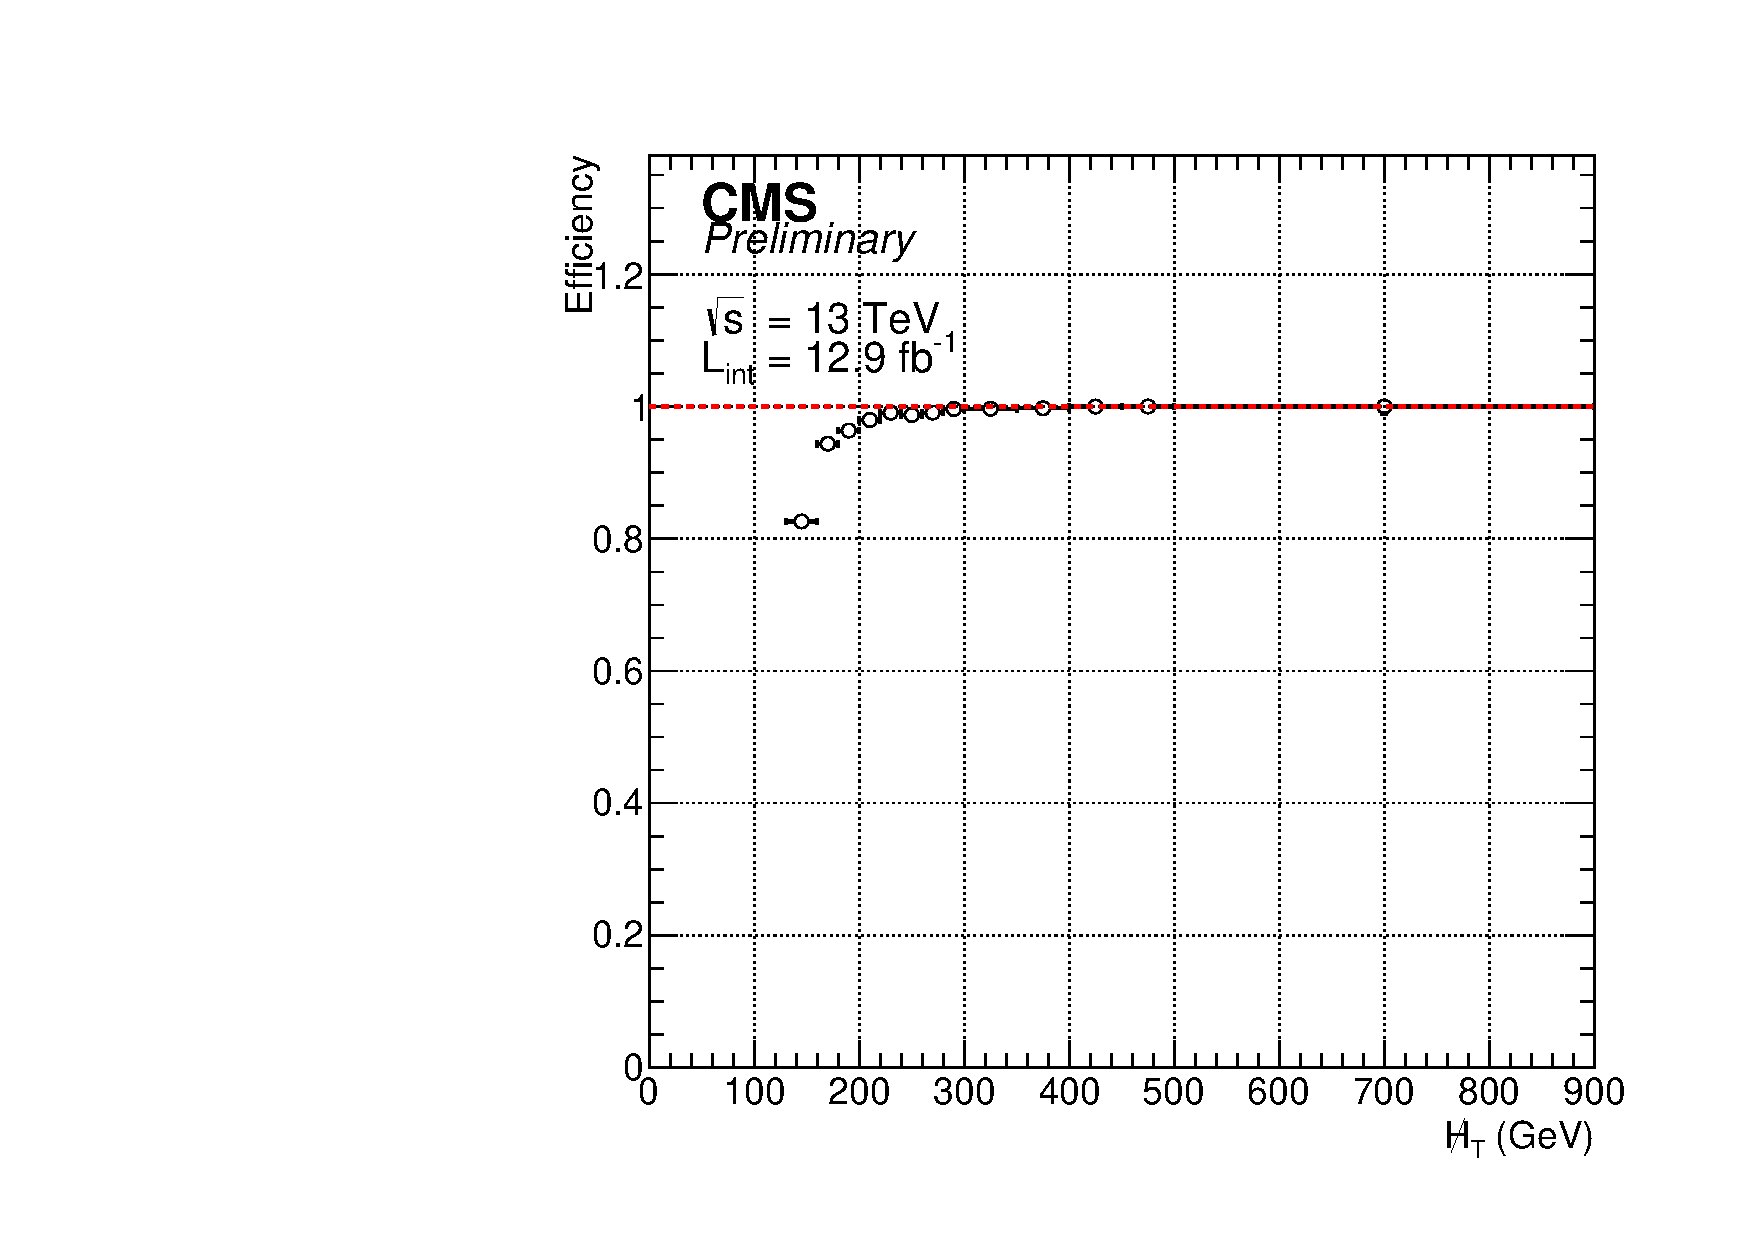
\includegraphics[width=0.4\textwidth]{figs/analysis/trigger/HLT_IsoMu22/HLT_AlphaTMonoAll_MoM_400to600_mht}} ~~\
    \subfloat[\gj region over all \HT]{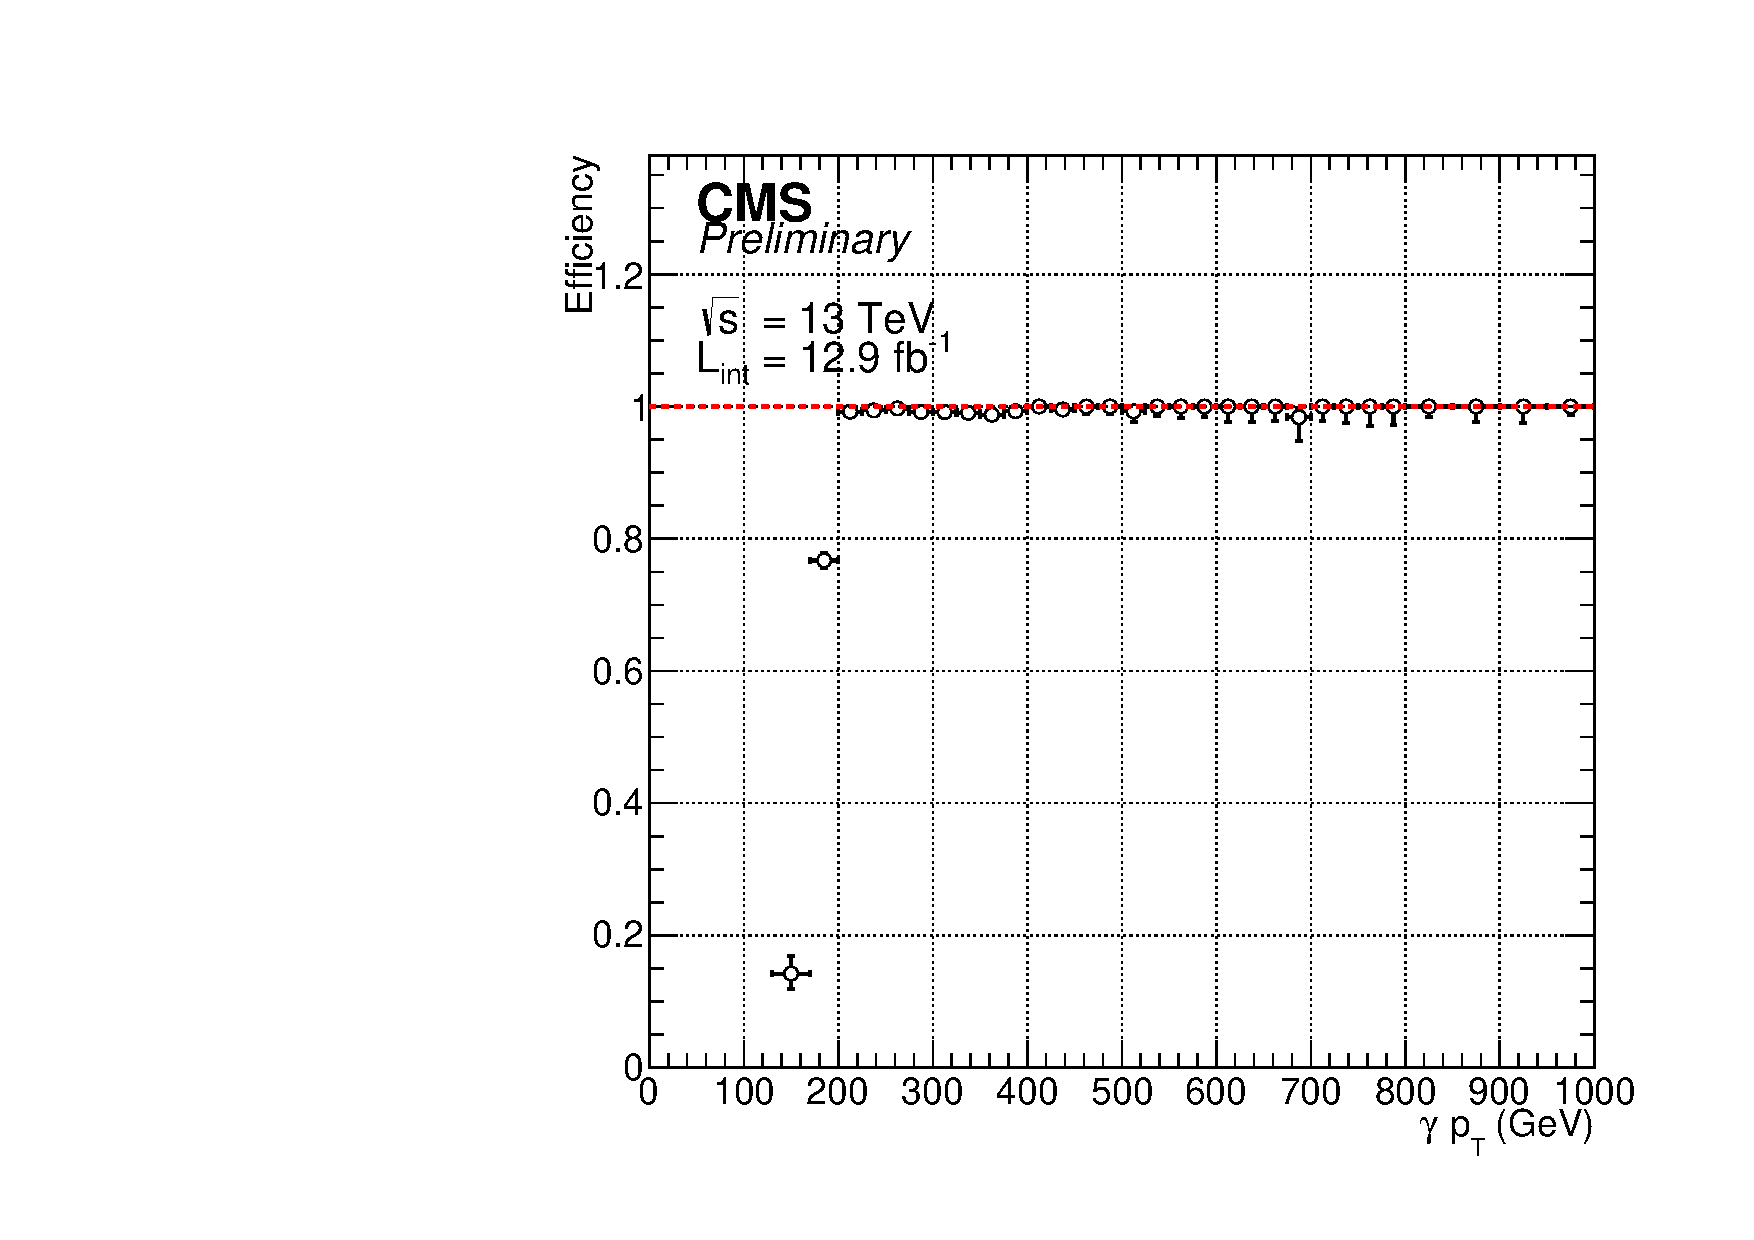
\includegraphics[width=0.4\textwidth]{figs/analysis/trigger/Photon/HLT_PhotonECALHT800_MoM_all_800to999999_gammapt}} \\ 
    \caption{Signal trigger efficiency in the \mht dimension measured
    with a muon sample (a) and \gj trigger efficiency measured with a
    hadronic sample (b).}
    \label{fig:trigEffsAt}
  \end{center}
\end{figure}

\subsection{Cross-section corrections}

The events considered within this analysis are selected
to have a high \HT and high \MET. The total number of events predicted
by the \MC simulation within this phase space does not agree with that
observed in data. To correct this, normalisation correction factors are
derived in \emph{sidebands} after all the other corrections have been
applied. This is particularly important in the case of the \gj simulation,
as the cross section for this process is only calculated to \LO
accuracy. For the other processes the cross section is calculated to
at least \NLO accuracy.

To derive the correction in the \gj control region, a sideband is used
in the \alphat variable. The same selection is applied as for the \gj
control region, other than the requirement that $0.50<\alphat<0.52$.
Within the \mj and \mmj control regions a sideband in \MHT is used,
requiring $100<\MHT<130~\gev$. A maximum likelihood fit across all the
sidebands is performed, where the yields for the \wj, \gj, \zmumu and
\ttbar processes are modelled as Poisson distributions. Within the fit
they are each allowed to be scaled by a free parameter. The
fit then finds the best scale factor for each sample to produce the
best data-simulation agreement within the sideband. These correction
factors can then be applied to the simulation throughout the rest of
the analysis. A summary of the correction factors can be seen in
Table~\ref{tab:sideband-corrs}.

\begin{table}[!h]
  \footnotesize
  \centering
  \caption{Cross section corrections for SM processes determined from
    data sidebands.}
  \label{tab:sideband-corrs}
  \begin{tabular}
    {lllc}
    SM process & Control sample & Data sideband           & Correction\T\B   \\
    \hline                   
    \gj        & \gj            & $0.50 < \alphat < 0.52$ & $1.33 \pm 0.03$\T \\
    \wj       & \mj            & $100 < \mht < 130\GeV$  & $1.13 \pm 0.01$   \\
    \zj      & \mmj           & $100 < \mht < 130\GeV$  & $0.99 \pm 0.02$   \\
    \ttbar     & \mj, \mmj      & $100 < \mht < 130\GeV$  & $0.86 \pm 0.01$\B \\
  \end{tabular}
\end{table}

The distributions of data and \MC simulated events for key analysis
variables in the major analysis regions are shown in
Appendix~\ref{app:charac}.  All of these plots are made after all the
corrections described in this section have been applied.

%%%%%%%%%%%%%%%%%%%%
\section{Background estimation for processes with genuine \MET} %day 2
\label{sec:bkgdMet}

The accurate determination of the \SM backgrounds is of utmost
importance when searching for the indications of \BSM phenomena. So as
not to rely too heavily on the modelling of the backgrounds in
simulation, a \emph{data-driven} approach is utilised wherever
possible. As this analysis is carried out with the requirement of
significant hadronic activity, mismodelling effects are particularly
prevalent due to the difficulties in simulating strong-force
interactions to a high degree of accuracy.

Given that the analysis selections are chosen to reduce the \QCD
multijet background to a negligible level, the significant \SM
backgrounds that must be predicted are those with genuine \MET in
their final state. The data-driven method used for predicting these
backgrounds is described in this section.

\subsection{Transfer factor method}
\label{sec:TF}

The control samples, defined in Sec.~\ref{sec:controlregions}, are
chosen to provide a collection of events in data that are in a phase
space that is close to that of the signal region. The control samples
are split into $(\HT,\nj,\nb)$ bins in a way that is equivalent to the
signal region, as introduced in Sec.~\ref{sec:categorisation}. Each
bin in a control region can then be extrapolated to the signal region
through the use of \emph{\TFs} that are derived from
simulation.  Each \TF is defined as a ratio of the yields
obtained from \MC simulation for the same bin of the signal region and
a given control sample:
\begin{equation}
  \label{equ:tf-ratio}
  {\rm TF} = \frac{N_{\rm MC}^{\rm signal}(\HT,\nj,\nb)}{N_{\rm
      MC}^{\rm control}(\HT,\nj,\nb)}, 
\end{equation}
where $N_{\rm MC}^{\rm signal}$ is the total simulated event yield for
all background processes in the signal region and $N_{\rm MC}^{\rm
control}$ is the equivalent event yield in a particular control
region.

Making use of these \TFs, predictions of background counts from \SM
processes, $\npre^{\rm signal}$, can then be made made based on the
various control samples:
\begin{equation}
  \label{equ:pred-method}
  \npre^{\rm signal}(\HT,\nj,\nb) = \frac{N_{\rm MC}^{\rm
      signal}(\HT,\nj,\nb)}{N_{\rm MC}^{\rm
      control}(\HT,\nj,\nb)} \times \nobs^{\rm
    control}(\HT,\nj,\nb),
\end{equation}
where $\nobs^{\rm control}$ is the number of events that are observed
within the bin of a control region.

When constructing the \TFs, the \MC expectations for the following \SM
processes are considered: W + jets ($N_{\rm W}$), \ttbar + jets
($N_{\ttbar}$), \znunu\ + jets ($N_{\znunu}$), DY + jets ($N_{\mathrm
DY}$), \gj ($N_\gamma$), single top + jets production via the $s$,
$t$, and $tW$-channels ($N_{\rm top}$), $WW+$~jets, $WZ~+$~jets, and
$ZZ + \textrm{jets}$ ($N_{\rm di-boson}$), and $\ttbar$V or $\ttbar$H
($N_{\rm {\ttbar}X}$). 

The \TFs account for differences in cross sections, acceptance,
reconstruction efficiencies and kinematic requirements between the
signal and control regions. One big advantage of using \TFs is that
any mismodelling effects that are consistent within a particular bin
across relevant \MC samples will cancel out. It is seen that the
mismodelling of hadronic effects typically vary as a function of \HT
and \nj. An example of this mismodelling is visible in
Fig.~\ref{fig:distribution_signal}, the disagreement in the data and
simulation changes as a function of the \HT or \nj. The fact
that the control samples are binned within these variables helps to
negate this issue, which is cancelled out within the \TF in each bin.
% Any dependence on \njet, \nb, or \HT is
% largely attributable to differences in acceptance due to the presence
% or otherwise of \alphat
% or \mht requirements.

\begin{figure}
    \begin{center}
        \subfloat {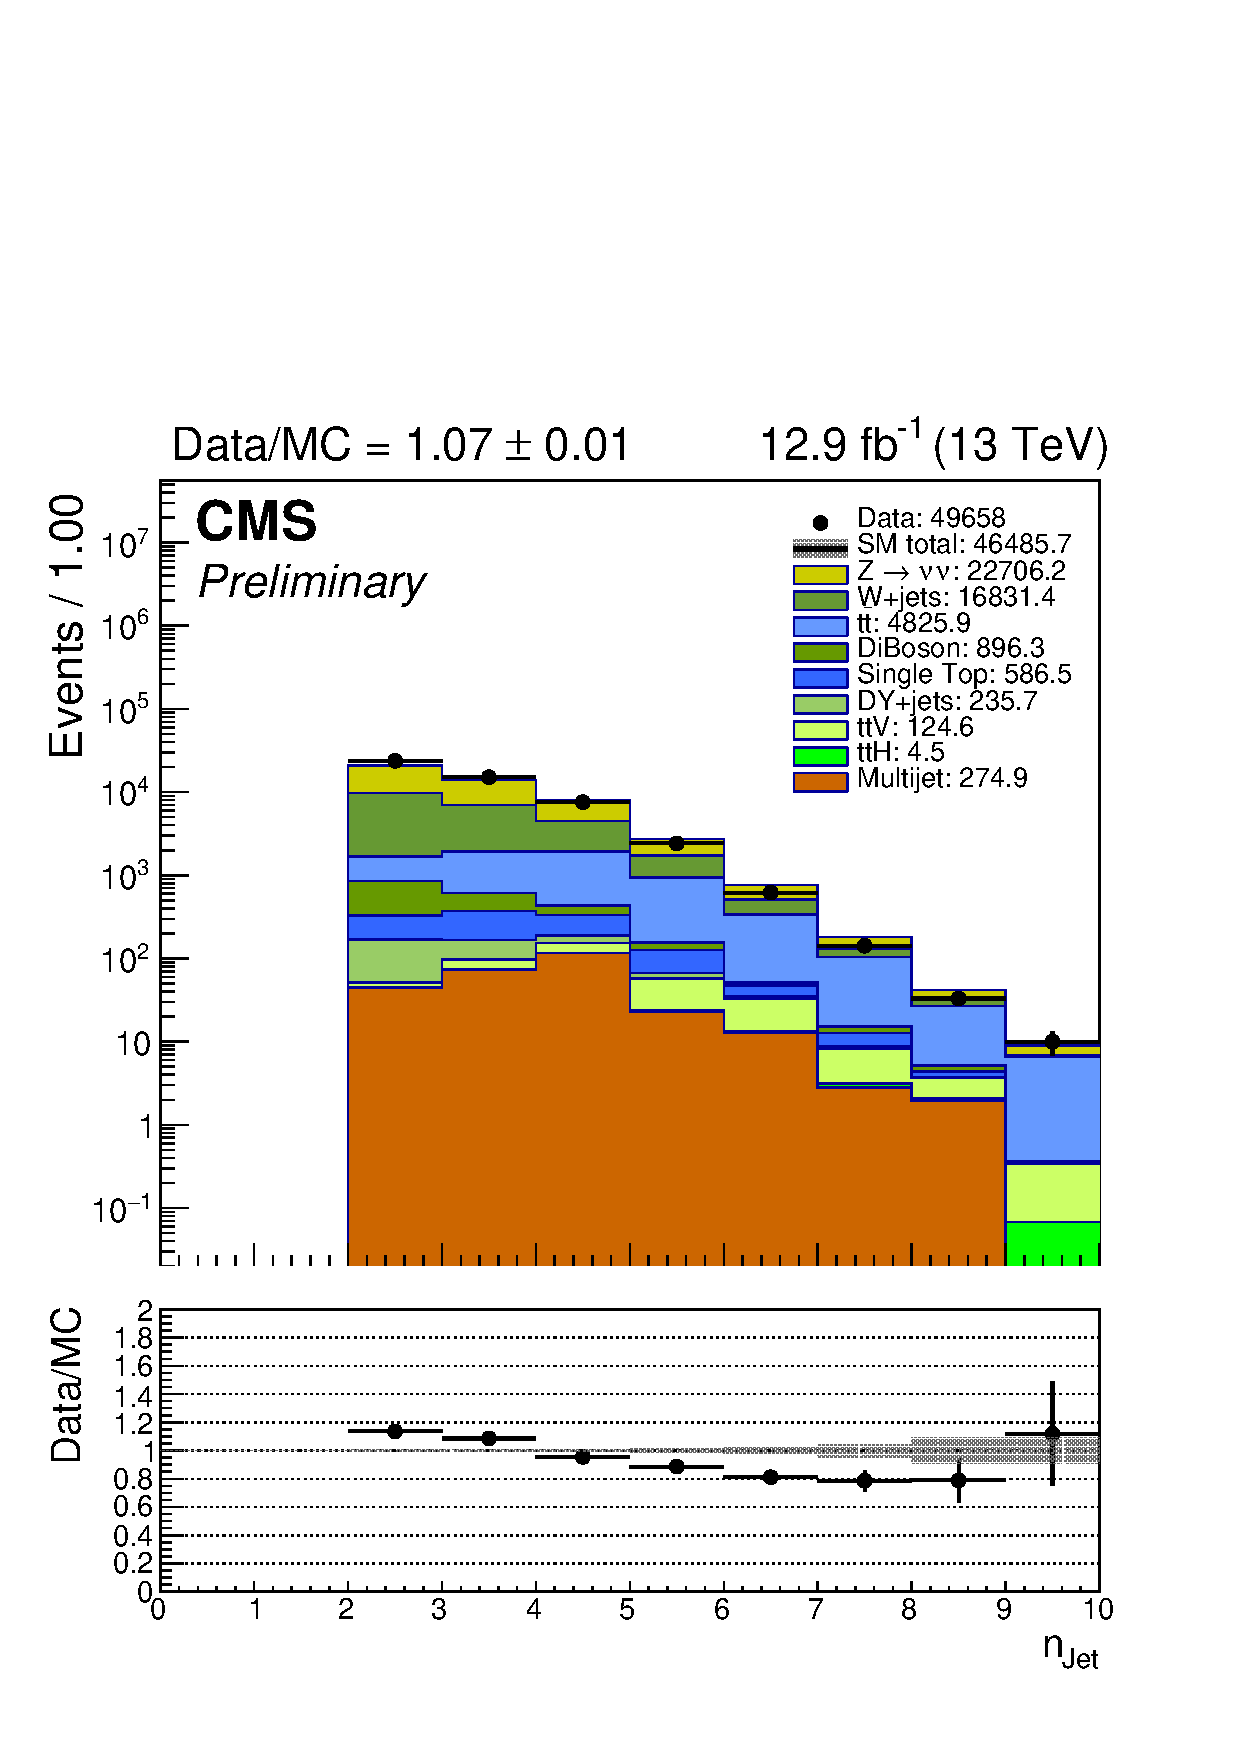
\includegraphics[width=0.5\textwidth]{figs/analysis/distributions/Signal/nJet40_sym.pdf}} ~~
        \subfloat {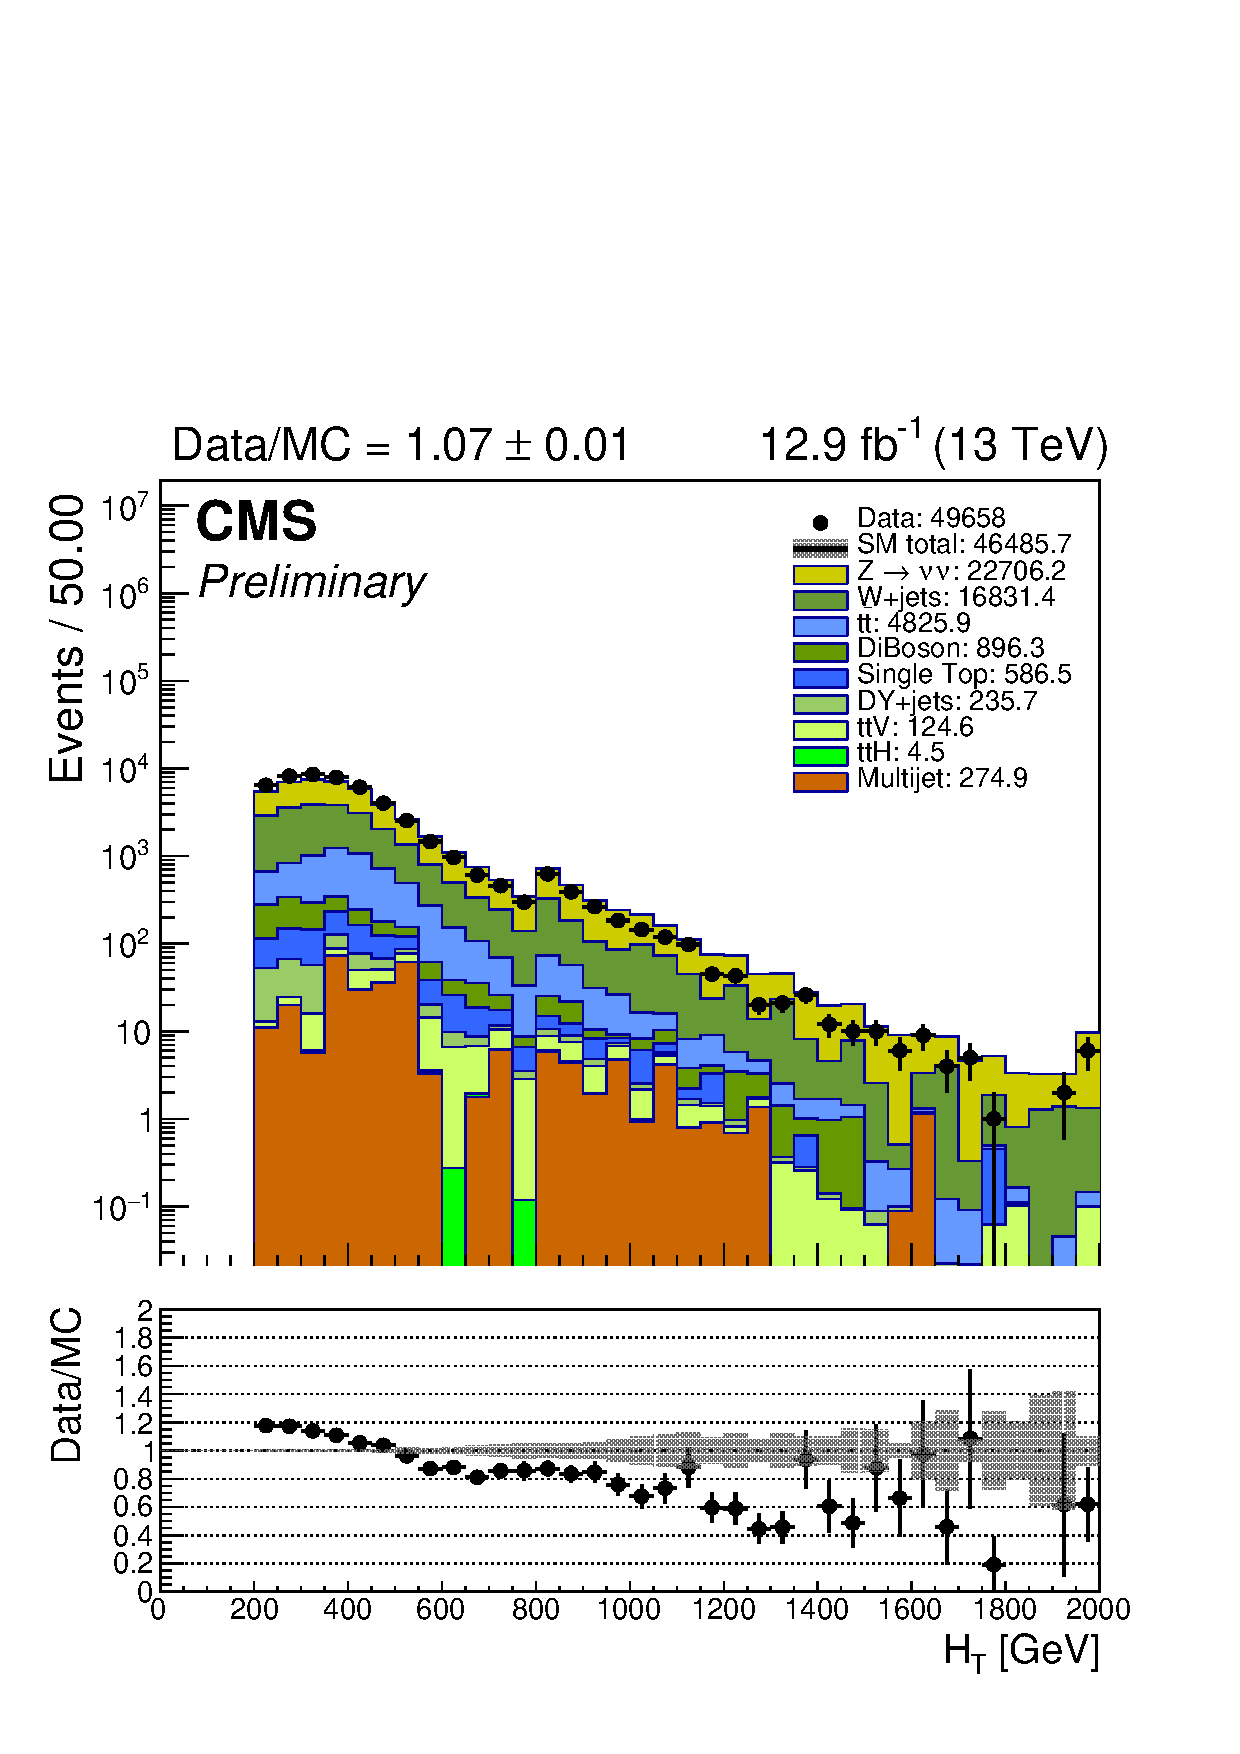
\includegraphics[width=0.5\textwidth]{figs/analysis/distributions/Signal/ht40_sym.pdf}} \\
        \caption{The \HT and \nj distributions in all categories of
        the signal region that have a symmetric jet topology}
        \label{fig:distribution_signal}
    \end{center}
\end{figure}

A systematic uncertainty is assigned to each \TF to account for
theoretical uncertainties and other mismodelling effects that do not
cancel in the ratio. Details of the specific systematic uncertainties
are given in Sec.~\ref{sec:systematics}.

Within the analysis, the \TF method is used with different control
regions to predict two different categories of background, the \znunu
and all the other remaining backgrounds. The \znunu background is
predicted with the \mmj, \gj and \mj control samples. The W, \ttbar and other residual
backgrounds are predicted with the \mj control sample. This method is
ultimately implemented within a fitting procedure that is defined
formally by the likelihood model described in
Sec.~\ref{sec:likelihood}. This procedure allows the appropriate
systematic uncertainties to be taken into a way that takes account of
their correlations across all samples and bins.

To summarise the fitting procedure, the observation in each bin of the
signal region is modelled as Poisson-distributed about the sum of a
\SM expectation (and a potential signal contribution). The components
of this SM expectation are related to the expected yields in the
control samples via the \TFs. The observations in each bin of the
control samples are similarly modelled as Poisson-distributed about
the expected yields for each control sample. In this way, for a given
bin, the observed yields in the signal and control samples are
connected via the transfer factors derived from simulation.  This
allows multiple control samples to modify the predicted yields in the
signal region within the constraints of their uncertainties.

\subsection{The \MHT dimension}
\label{sec:mhtDim}

The \TF method is used to estimate the total background counts in each
of the (\HT,\nj,\nb) bins. However, to maximise the sensitivity to
\BSM signatures with large missing momentum, events in the analysis are also
categorised based on their \MHT. Due to limitations on the
number of events available in each control sample, it is
disadvantageous to add another binning
dimension. This would result in statistical uncertainties of the
control region event counts dominating the background prediction.
Instead, the shape of the \MHT distribution is taken directly from
simulation for each of the (\HT,\nj,\nb) bins in the signal region.
This is justified by the fact that binning in these variables helps to
isolate hadronic mismodelling effects within each bin, which then
cancel in the \TFs. 

% When looking at the \mht dimension inclusively in \scalht there are
% large theoretical uncertainties that originate from mixing events
% at different scales. These uncertainties can be mitigated if the events 
% are binned according to a variable, such as \scalht, 
% which is strongly correlated with the scale of the event. 
% After this categorisation is applied, the uncertainty in 
% the distribution of the \mht variable
% (as well as any other MET-like variable) is expected to be 
% mainly affected by the MC modelling of the particle 
% decays and, to a lesser extent, by jet reconstruction effects, 
% such as jet energy scale and resolution. 
% This approach, which will be often referred to as \textit{scale anchoring}
% in the following, is used in this analysis. The distribution in \mht
% is measured in data using the control regions and compared to MC
% to determine the validity of the zero bias hypothesis after scale anchoring.

To make sure that this approach is valid, the assumption that the \MHT
dimension is well modelled in each bin must be tested. This testing is
carried out within the \gj, \mj and \mmj control regions. Within each
analysis bin of each of the control regions, the shape of the \MHT
distribution in data is compared to the distribution in \MC
simulation. The normalisation can be disregarded as it is set through the
\TF method.  Provided the modelling is reasonable, the ratio of the
normalised shapes is expected to have a value of one consistently
across the \MHT dimension, in each of the (\HT,\nj,\nb) bins. Any
difference is used to derive a systematic uncertainty on the \MHT
shape as described in Sec.~\ref{sec:systMht}. 

An example of the data/\MC ratio as a function of the \MHT for two
representative bins is shown in Fig.~\ref{fig:linearFitExamples}. The
result of a constant and linear fit and their respective uncertainties
are drawn on the plots in blue and red respectively. To ensure that a
flat hypothesis of the ratio is valid across all bins, the significance
of the deviation from zero of the linear parameters of the data/\MC
fits is shown in Fig.~\ref{fig:pulls}. As they are compatible with no
linear dependence, the use of simulation to determine the \MHT shape
in each (\HT,\nj,\nb) category is considered valid.

\begin{figure}[h!]
  \centering
  \subfloat[\gj, $\nb=1$, $\nj=2$ symmetric category and \scalht 400-500\GeV bin]{
    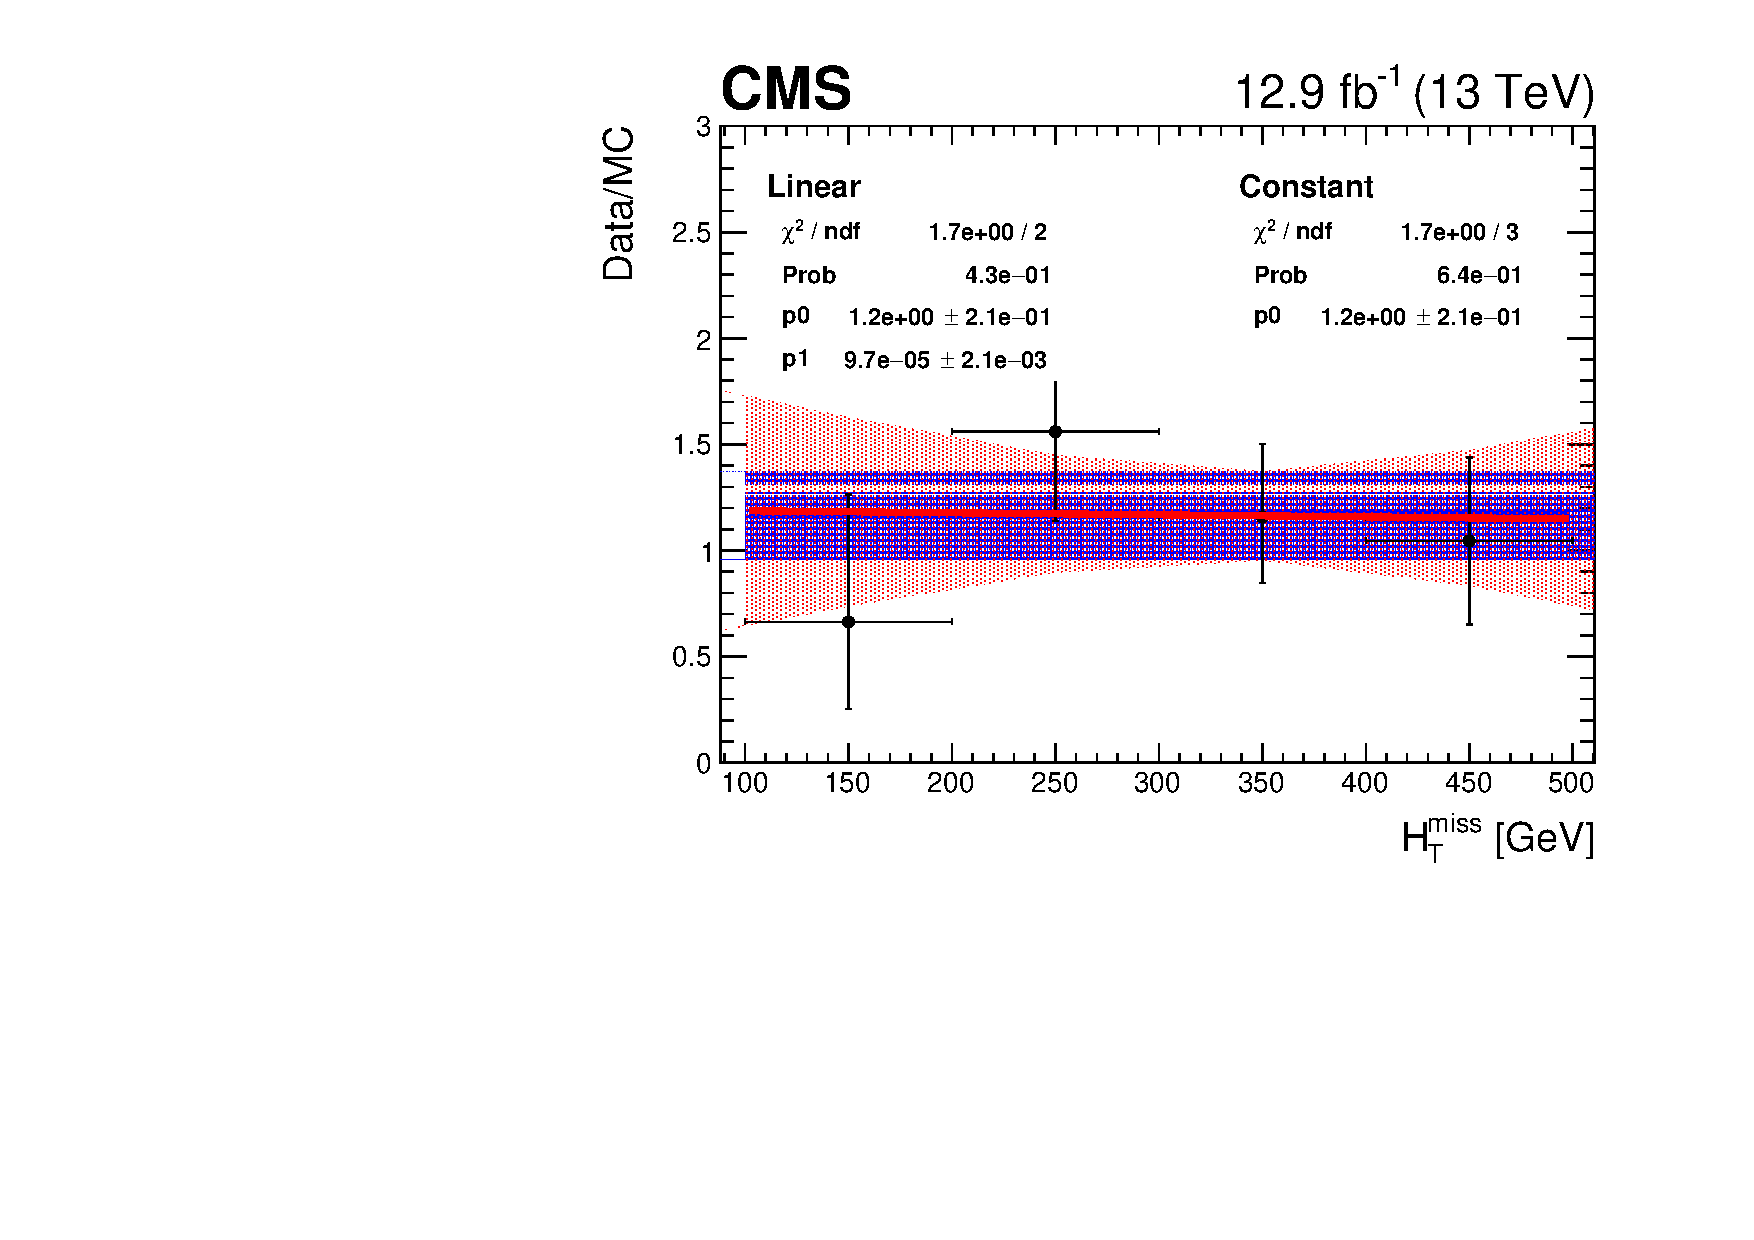
\includegraphics[width=0.5\textwidth]{figs/analysis/mhtShape/mht_eq1b_eq2j_ht_400_500_SinglePhoton_Graph}
  }~~
  \subfloat[\mmj, $\nb=0$, $\nj=3$ asymmetric category and \scalht 300-350\GeV bin]{
    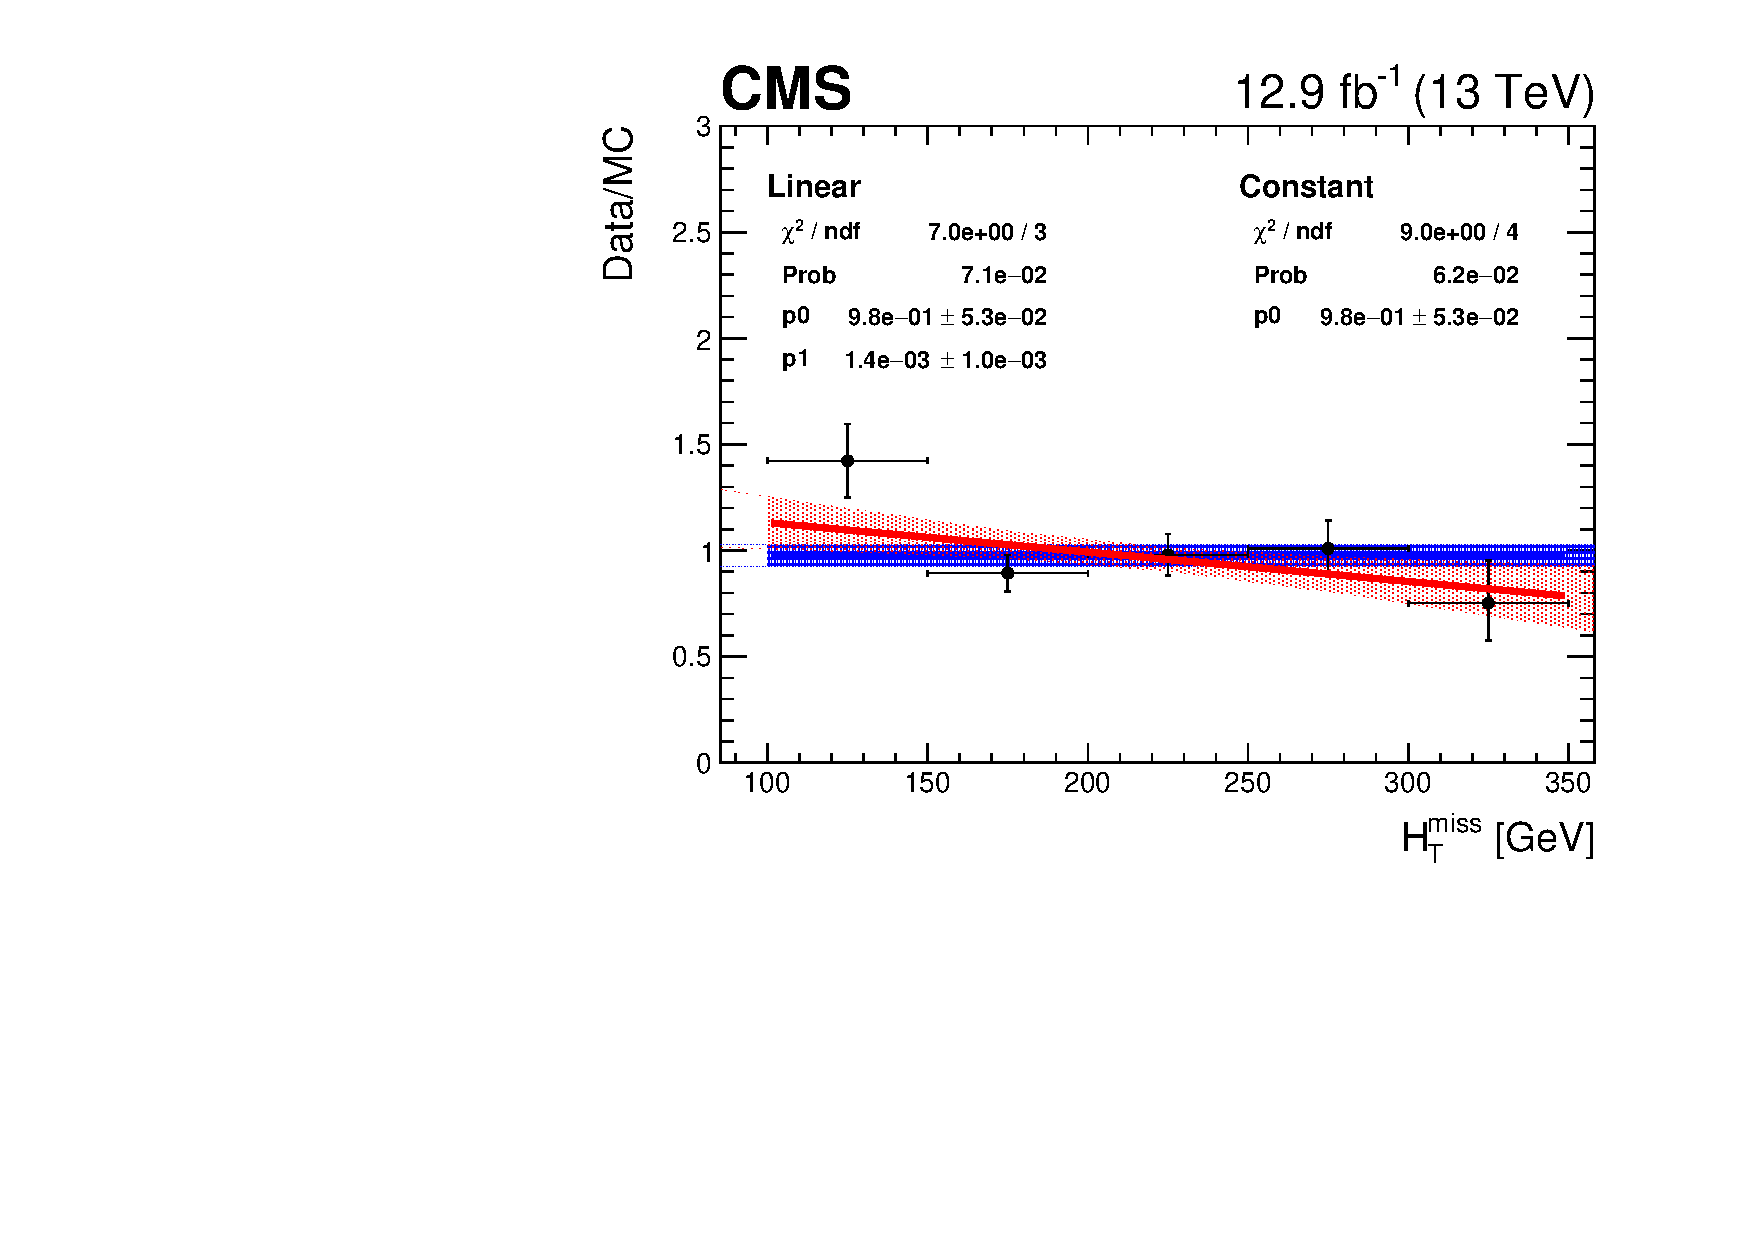
\includegraphics[width=0.5\textwidth]{figs/analysis/mhtShape/mht_eq0b_eq3a_ht_300_350_DoubleMu_Graph}
  }\\
  \caption{ 
  The data/MC distribution against \mht (denoted $H_T^{miss}$) for two
  representative categories in the \gj (a) and \mjj (b) control regions.
  Linear and constant fits are made to the ratio and their p-value and
  fit parameters are shown on the plot.
  }
  \label{fig:linearFitExamples}
\end{figure}

\begin{figure}[h!]
  \centering
  \subfloat[\mj]{
    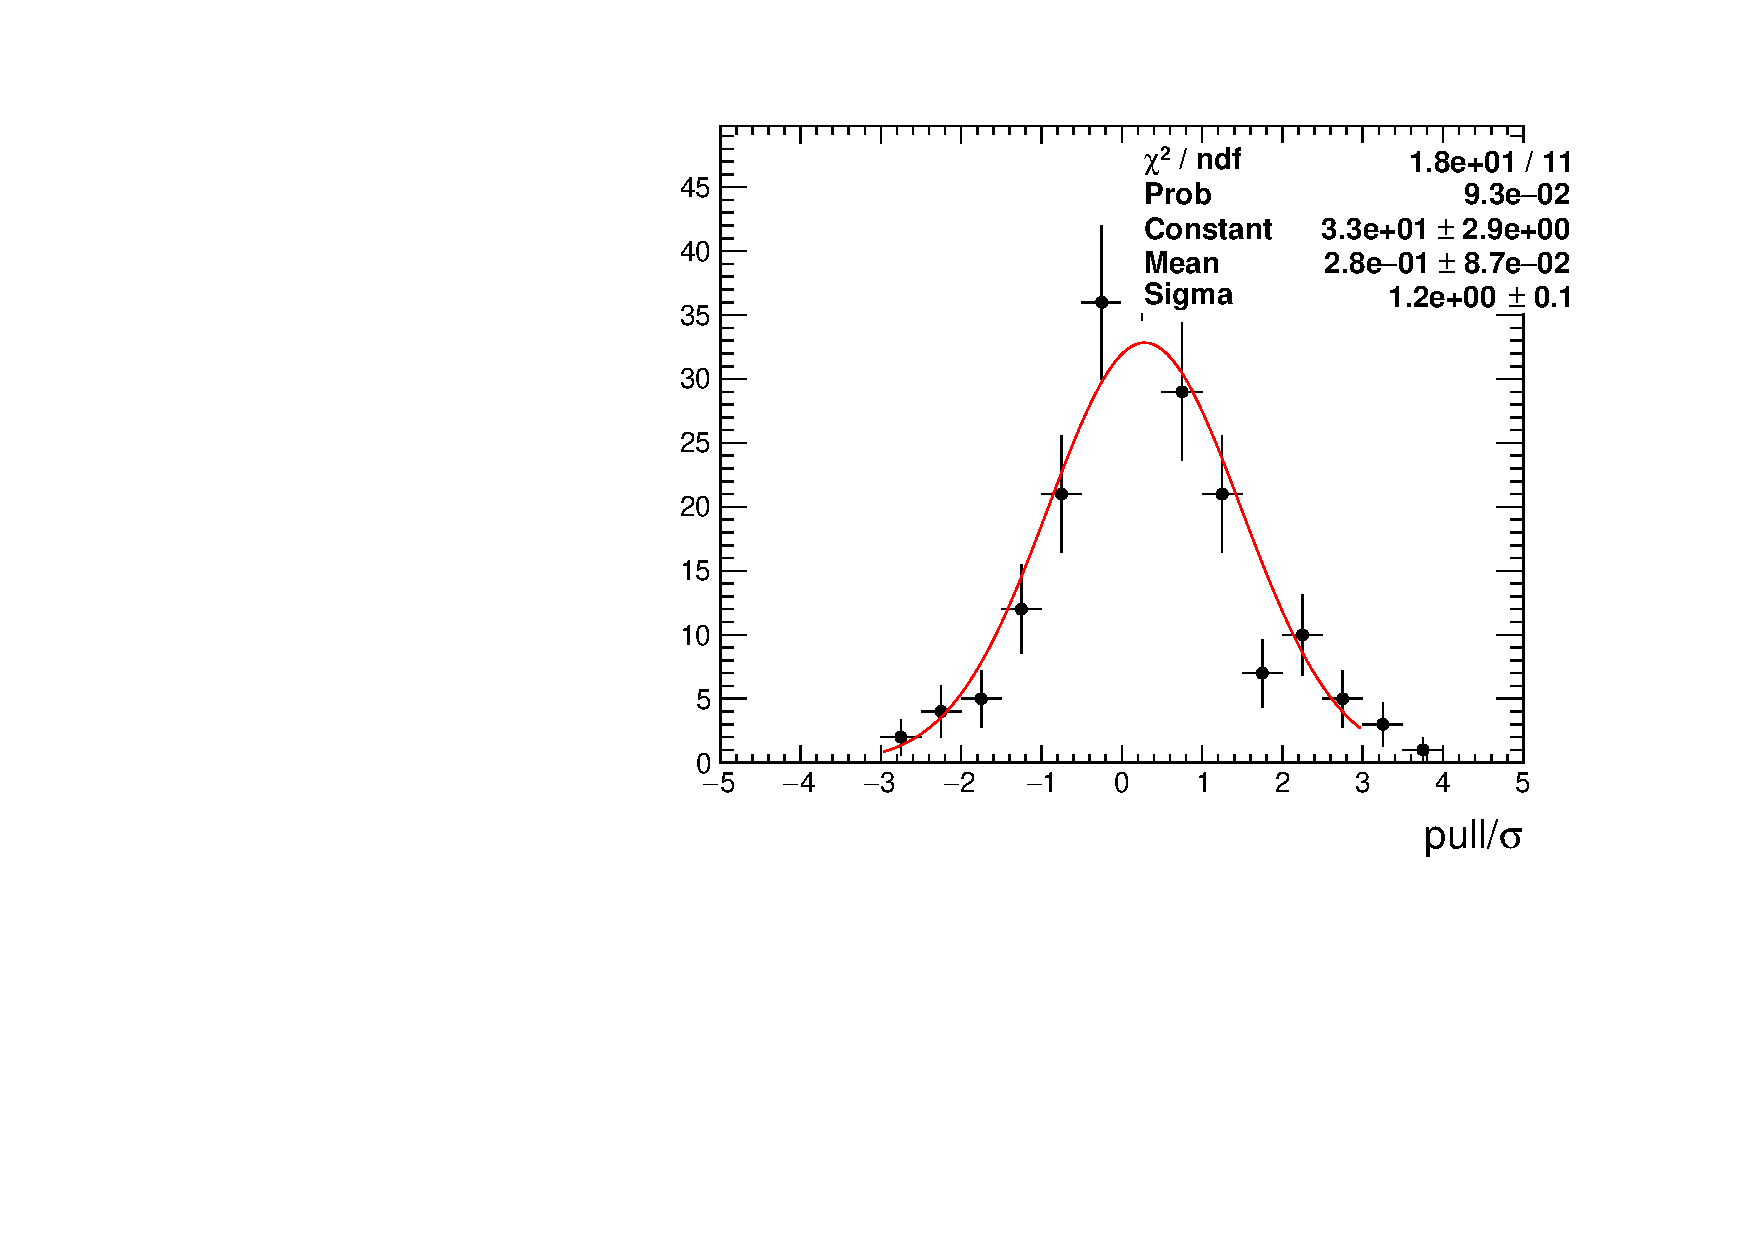
\includegraphics[width=0.5\textwidth]{figs/analysis/mhtShape/pull_Linear2DShiftMean_p1_SingleMu.pdf}
  }~~
  \subfloat[\gj]{
    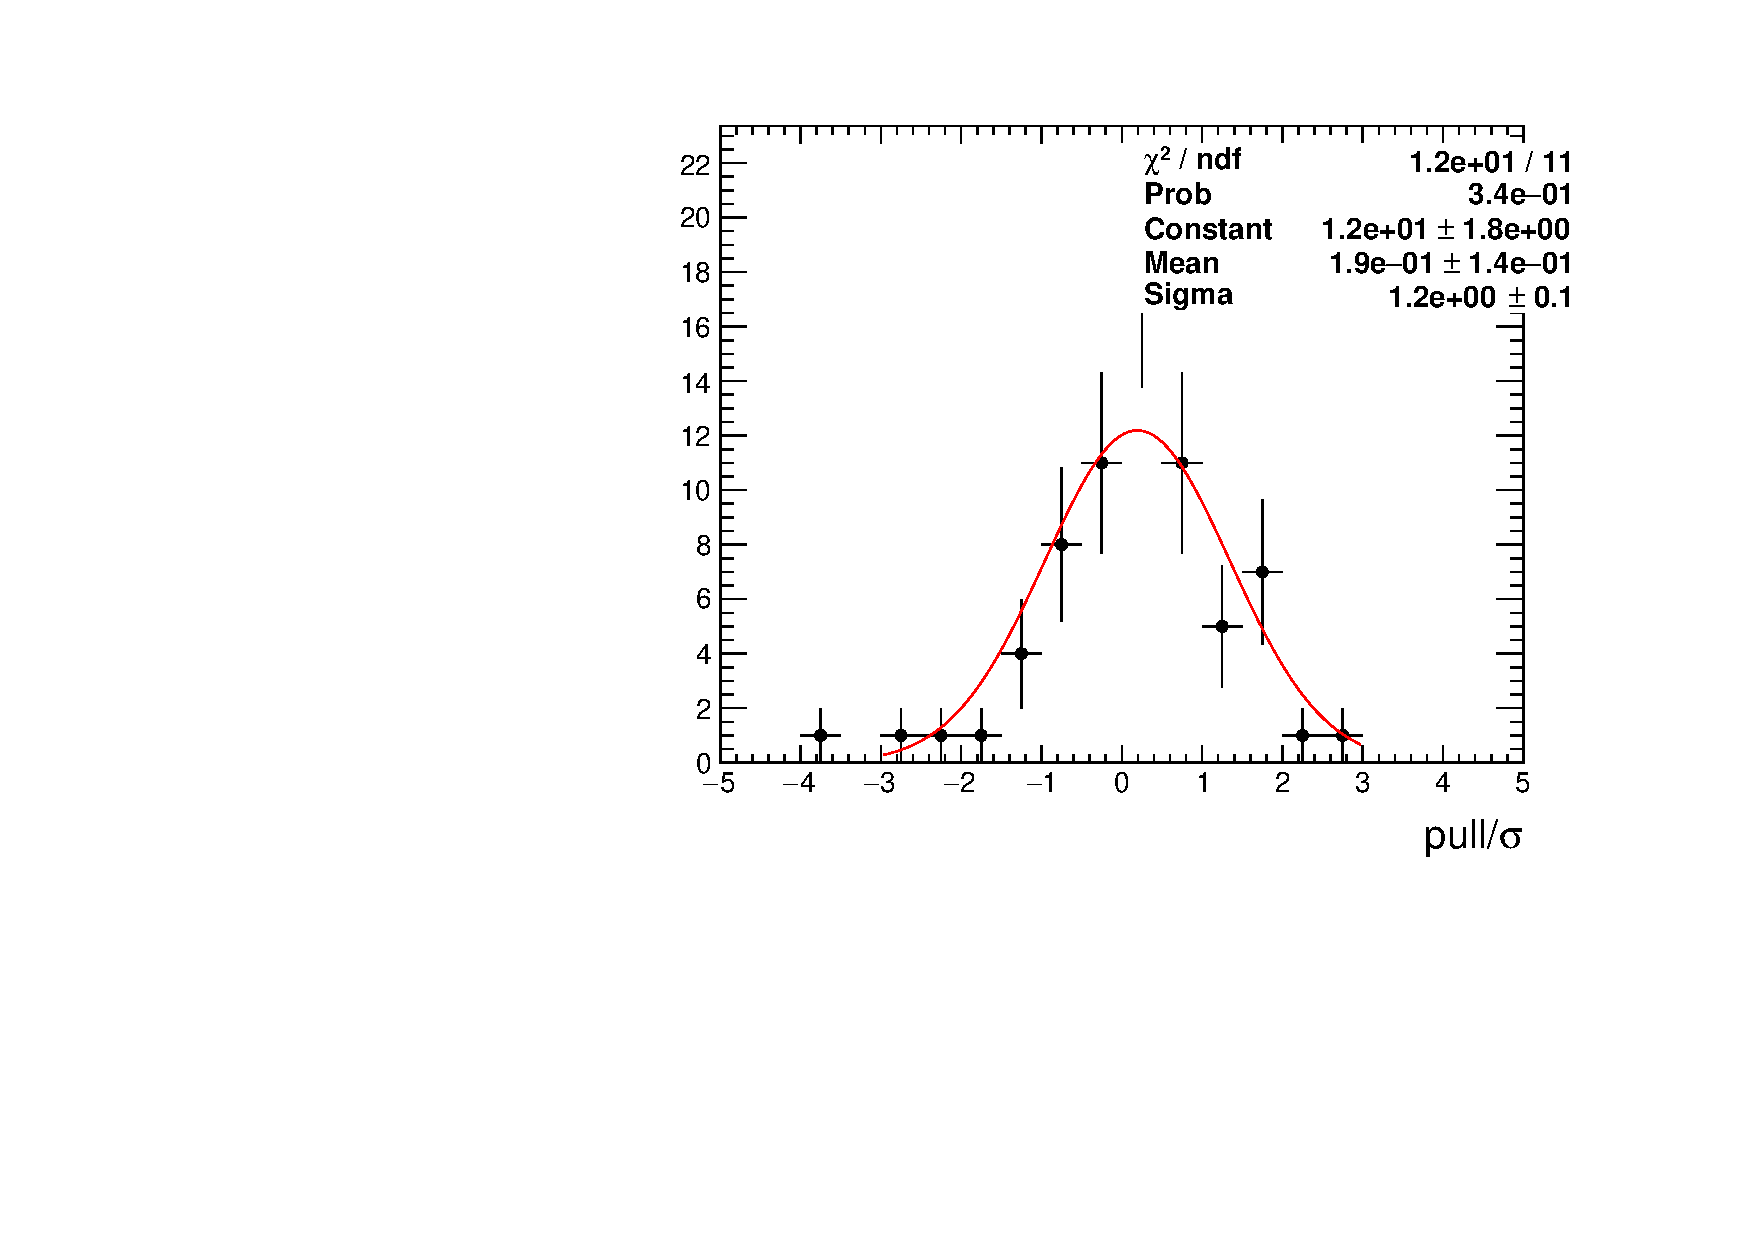
\includegraphics[width=0.5\textwidth]{figs/analysis/mhtShape/pull_Linear2DShiftMean_p1_SinglePhoton.pdf}
  }\\
  \subfloat[\mmj]{
    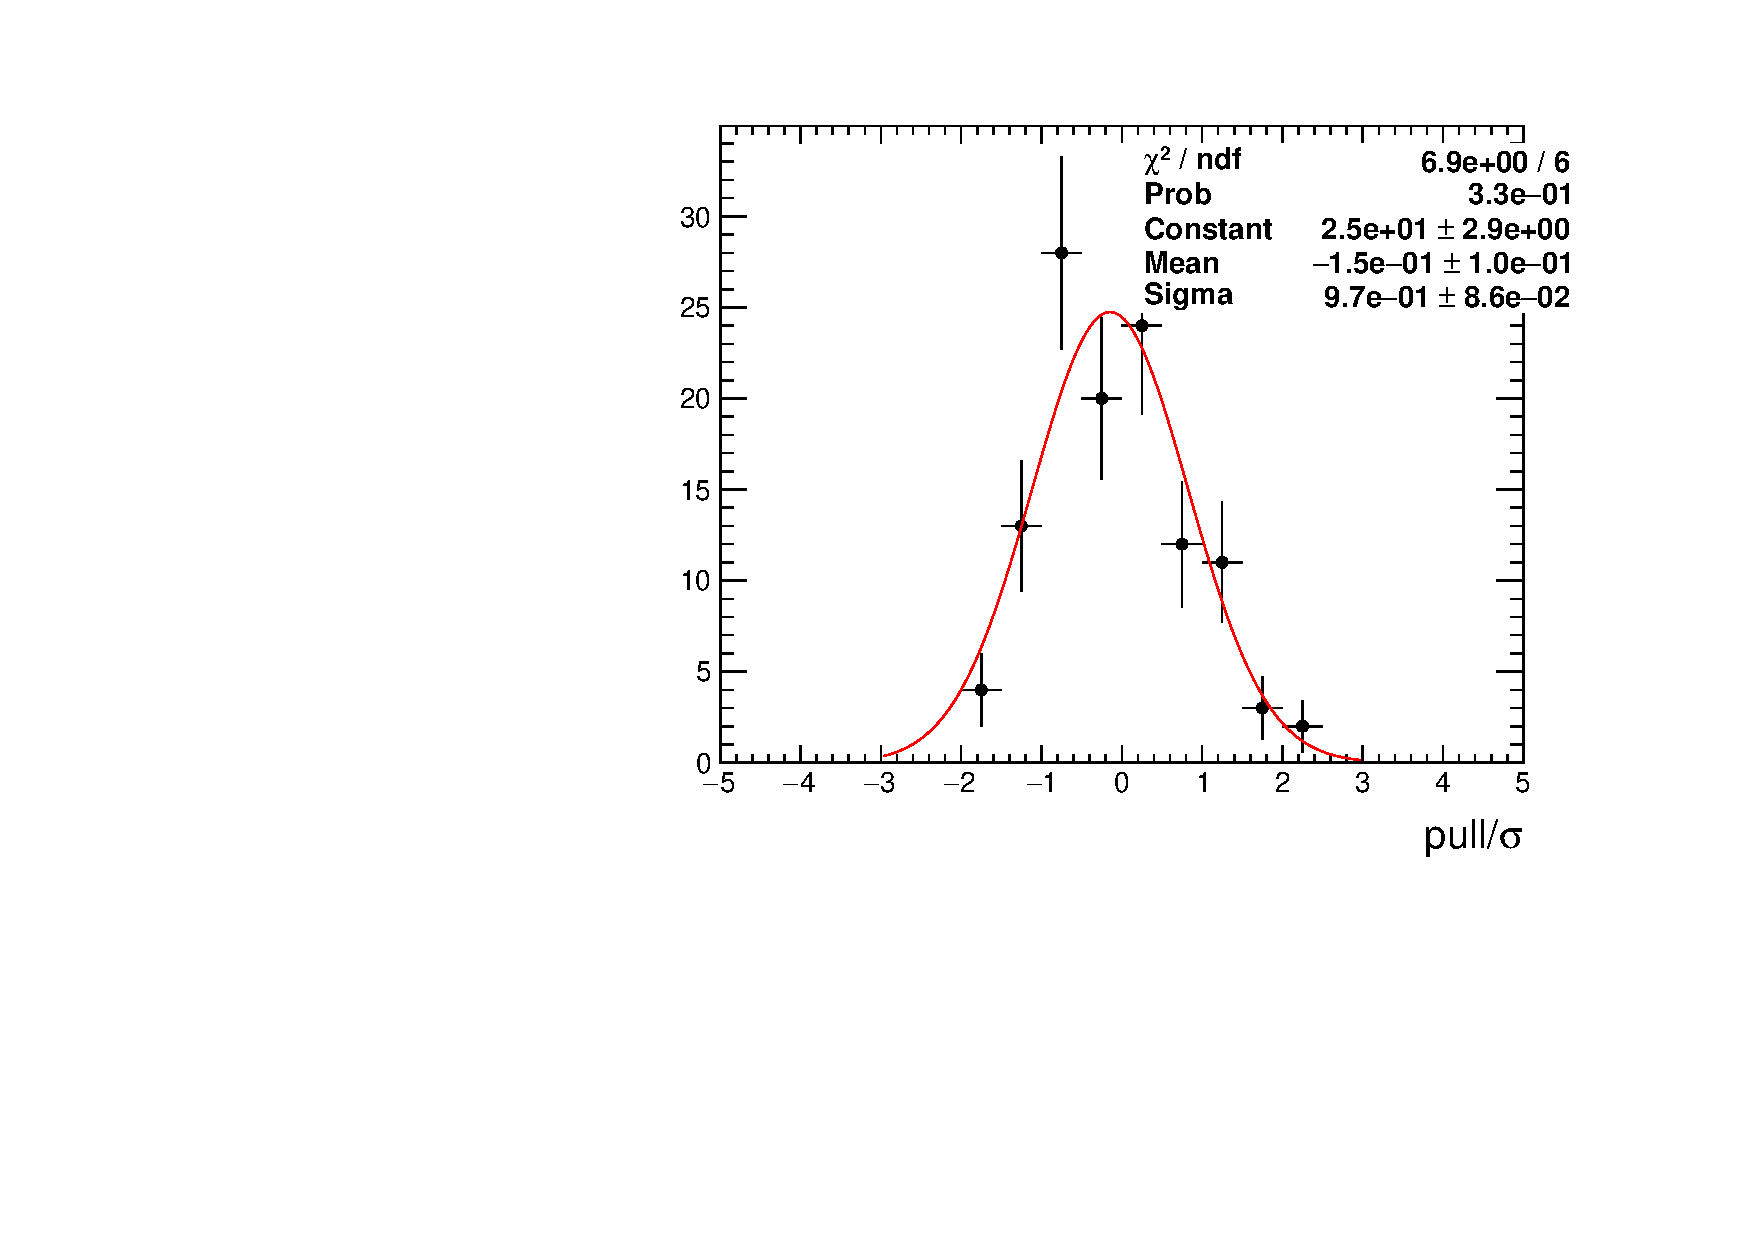
\includegraphics[width=0.5\textwidth]{figs/analysis/mhtShape/pull_Linear2DShiftMean_p1_DoubleMu.pdf}
  }~~
  \\
  \caption{
  The distribution of the significance of the deviation from zero of
  the linear parameters of the . As all these pulls for each of the
  control regions are statistically compatible with one, a linear
  hypothesis for the \MHT data/\MC ratio is valid.}
  \label{fig:pulls} 
\end{figure}

The size of the \MHT bins within the signal region are chosen to
contain enough data counts within each of the control regions to
perform the validation. Taking \MHT bin widths of 50~\gev are found
to be enough to satisfy this condition, while not being limited by the
measured \MHT resolution. In most cases the \MHT bins
are naturally bounded from above by maximum value of \HT in a
particular bin.  However, the highest \HT bin is unbounded from above,
the final \MHT bin is therefore limited to sit at $\MHT>800~\gev$
($\MHT>600~\gev$) for symmetric (asymmetric) topologies to
ensure the requisite statistics. All of the bins used are listed in
Appendix~\ref{app:mhtBinning}.
% determine the binning constraints based on a minimum number of
% events for stats in the CRs

%%%%%%%%%%%%%%%%%%%%
\section{Background estimation for QCD multijet processes} %day4
\label{sec:qcdEstimation}

% copy and paste in from AN?
As discussed extensively in Chapter~\ref{chap:selection}, the strategy
of the analysis is based around reducing the \QCD multijet background
to a negligible level. However, it is necessary to verify that the
multijet contribution within the signal region is indeed small. This
is confirmed with the method described in this section. To remain
sensitive to small contributions in the signal region from \BSM
phenomena, it is imperative to keep the uncertainties on the level of
\QCD contamination small. The method therefore utilises data-driven
techniques, similar to those used for the estimation of processes with
genuine \MET described in Sec.~\ref{sec:TF}.

\subsection{QCD-enriched sidebands}
%trigger efficiencies?

To be able to carry out a data-driven estimate, three data sidebands
to the signal region are defined. They are chosen to be heavily \QCD
contaminated, but still close in phase space to the signal region. To
achieve this, the signal region selection is applied with the
requirements on two of the variables used to remove the multijet
background inverted. They are defined by the requirement 
$\mhtmet>1.25$, $\bdphi<0.5$ and both these requirements as
illustrated in Table~\ref{tab:qcd_sidebands}. 

For the core \QCD multijet background prediction, the \mhtmet sideband
is used to estimate the \QCD yields in the signal region through an
extrapolation with a \TF. To then carry out a validation of the
transfer factor, the \bdphi and double sidebands are used.

\begin{table}[h!]
  \caption{Definition of sidebands used in the determination of the
    QCD background contributions in the signal region. }
  \label{tab:qcd_sidebands}
  \centering
  \footnotesize
  \begin{tabular}{ l|l|l }
                           & $\bdphi < 0.5$           & $\bdphi > 0.5$                  \\[0.2ex]
    \hline
    $1.25 < \mhtmet < 3.0$ & \textbf{A} Double sideband & \textbf{B} \mhtmet sideband \\[0.2ex]
    \hline
    $\mhtmet < 1.25$       & \textbf{C} \bdphi sideband & \textbf{D} Signal region    \\[0.2ex]
  \end{tabular}
\end{table}
% {\bf FIXME} put something here from Xtian's studies? ie how they're
% broken down into different mismeasurements?

%\subsection{The \QCD multijet background estimation method}
\subsection{The method}
\label{sec:qcdMethod}

The method makes use of the ratio of simulated \QCD counts in the
signal region to the \mhtmet sideband, \rmhtmet, per (\HT,\nj) bin.
This is essentially a \TF constructed from the \QCD simulation.
Each ratio is used as a multiplier on the predicted \QCD counts per
bin in the \mhtmet data sideband.  These data counts are collected
with the signal region triggers described in Sec.~\ref{sec:trigStrat}. 

The prediction of the number of \QCD multijet events in
the sideband, $\mathcal{Q}$, is carried out with a maximum likelihood fit analagous to
that described in Sec.~\ref{sec:likelihood}, but in the \mhtmet
sideband and with the total number of \QCD events free to be
determined. In this fit,
the electroweak backgrounds within the sideband are determined with the method described
in Sec.~\ref{sec:bkgdMet} with \mj, \mmj and \gj
control regions that have the same selection as the control
regions described in Sec.~\ref{sec:controlregions}, apart from an inverted
\mhtmet cut. All relevant systematic uncertainties on the \TFs,
described in Sec.~\ref{sec:systematics} are taken into account.  After the
contribution of the electroweak backgrounds is estimated, the
remaining data counts are attributed to \QCD. In this prediction, all
counts and predictions are inclusive in \nb and \MHT. The product of these
predicted \QCD counts and the ratio, $\mathcal{Q} \times \rmhtmet$,
provides an estimate of the level of \QCD multijet events in each
(\HT,\nj) bin of the signal region. 

\begin{figure}[!h]
  \centering
  \subfloat[Simulated \QCD events in signal region.\label{fig:qcd_pass}]{
    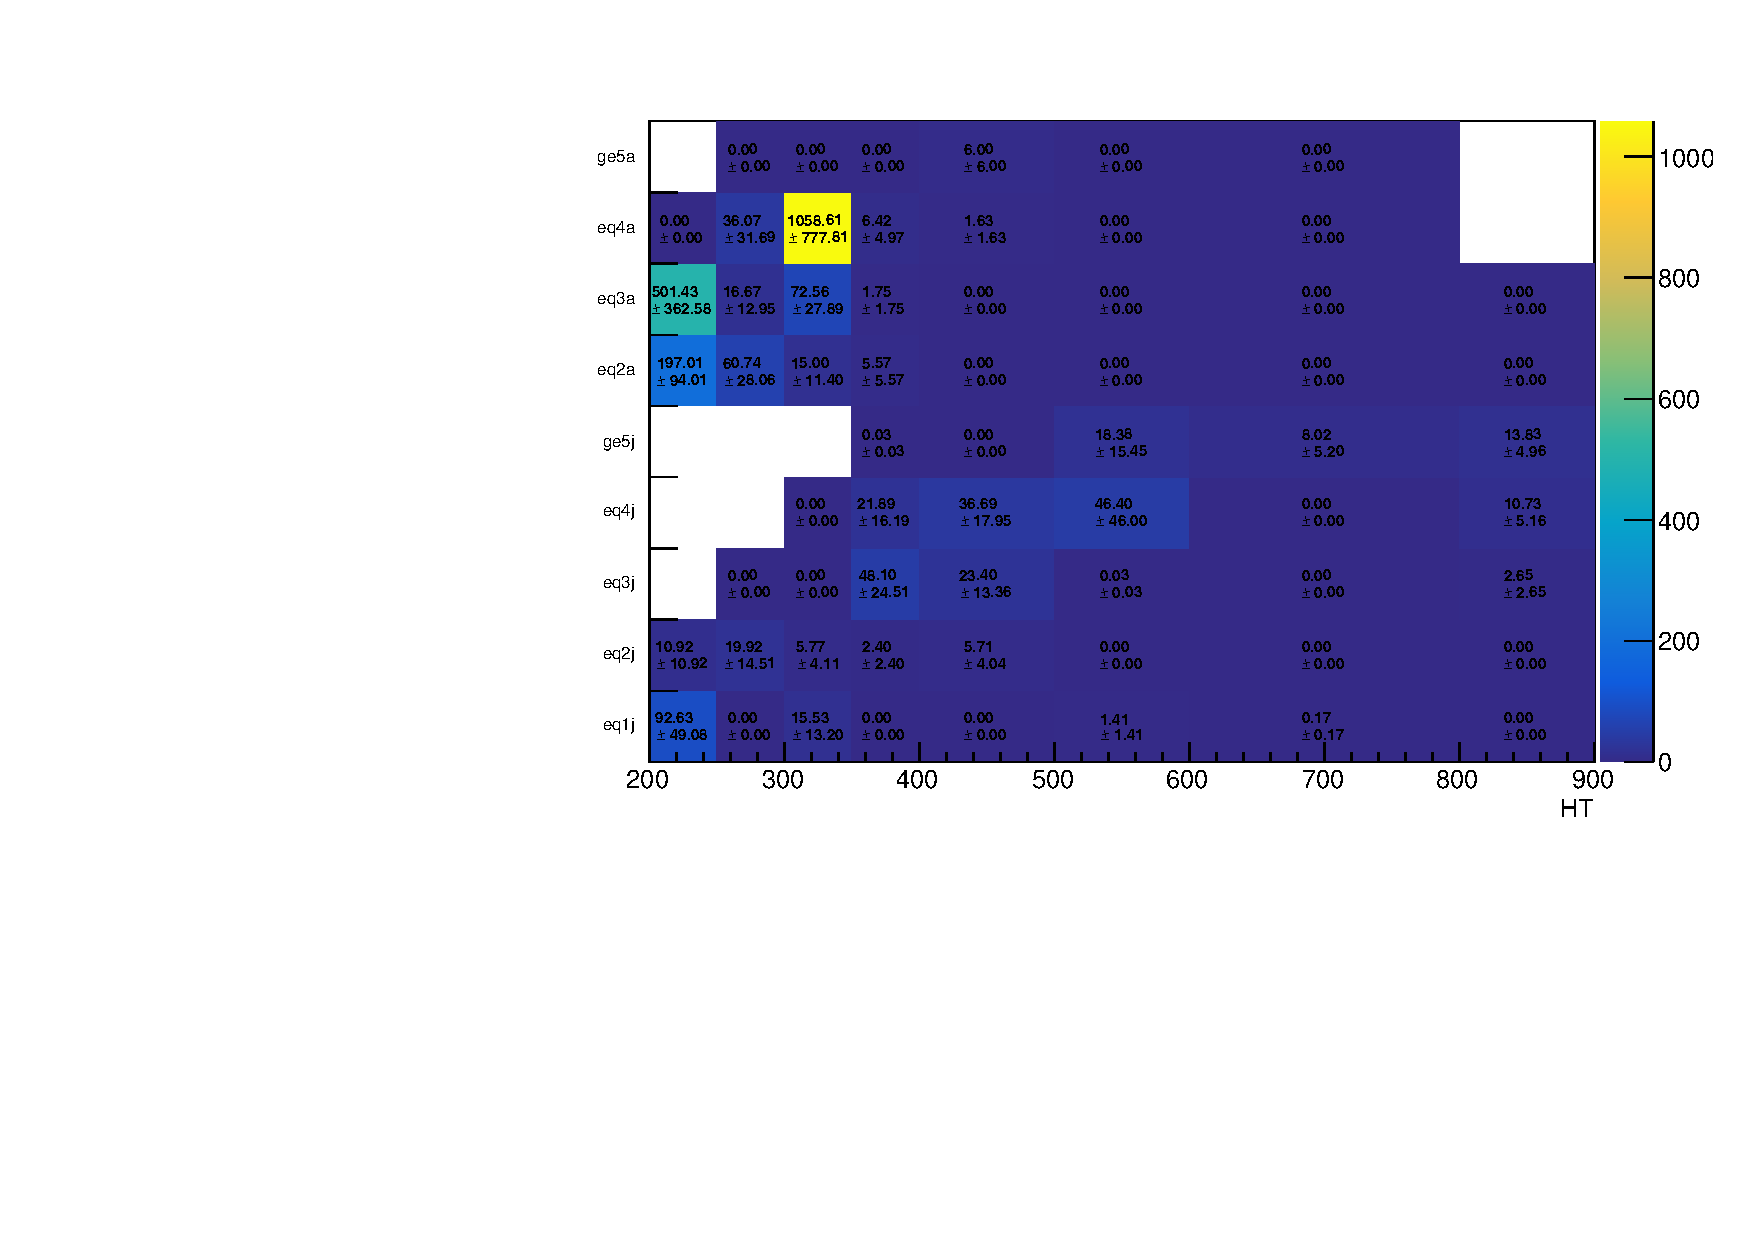
\includegraphics[width=0.5\textwidth]{figs/analysis/qcdMethod/signalQCD_MC}
  } 
  \subfloat[Simulated \QCD events in \mhtmet sideband.\label{fig:qcd_fail}]{
    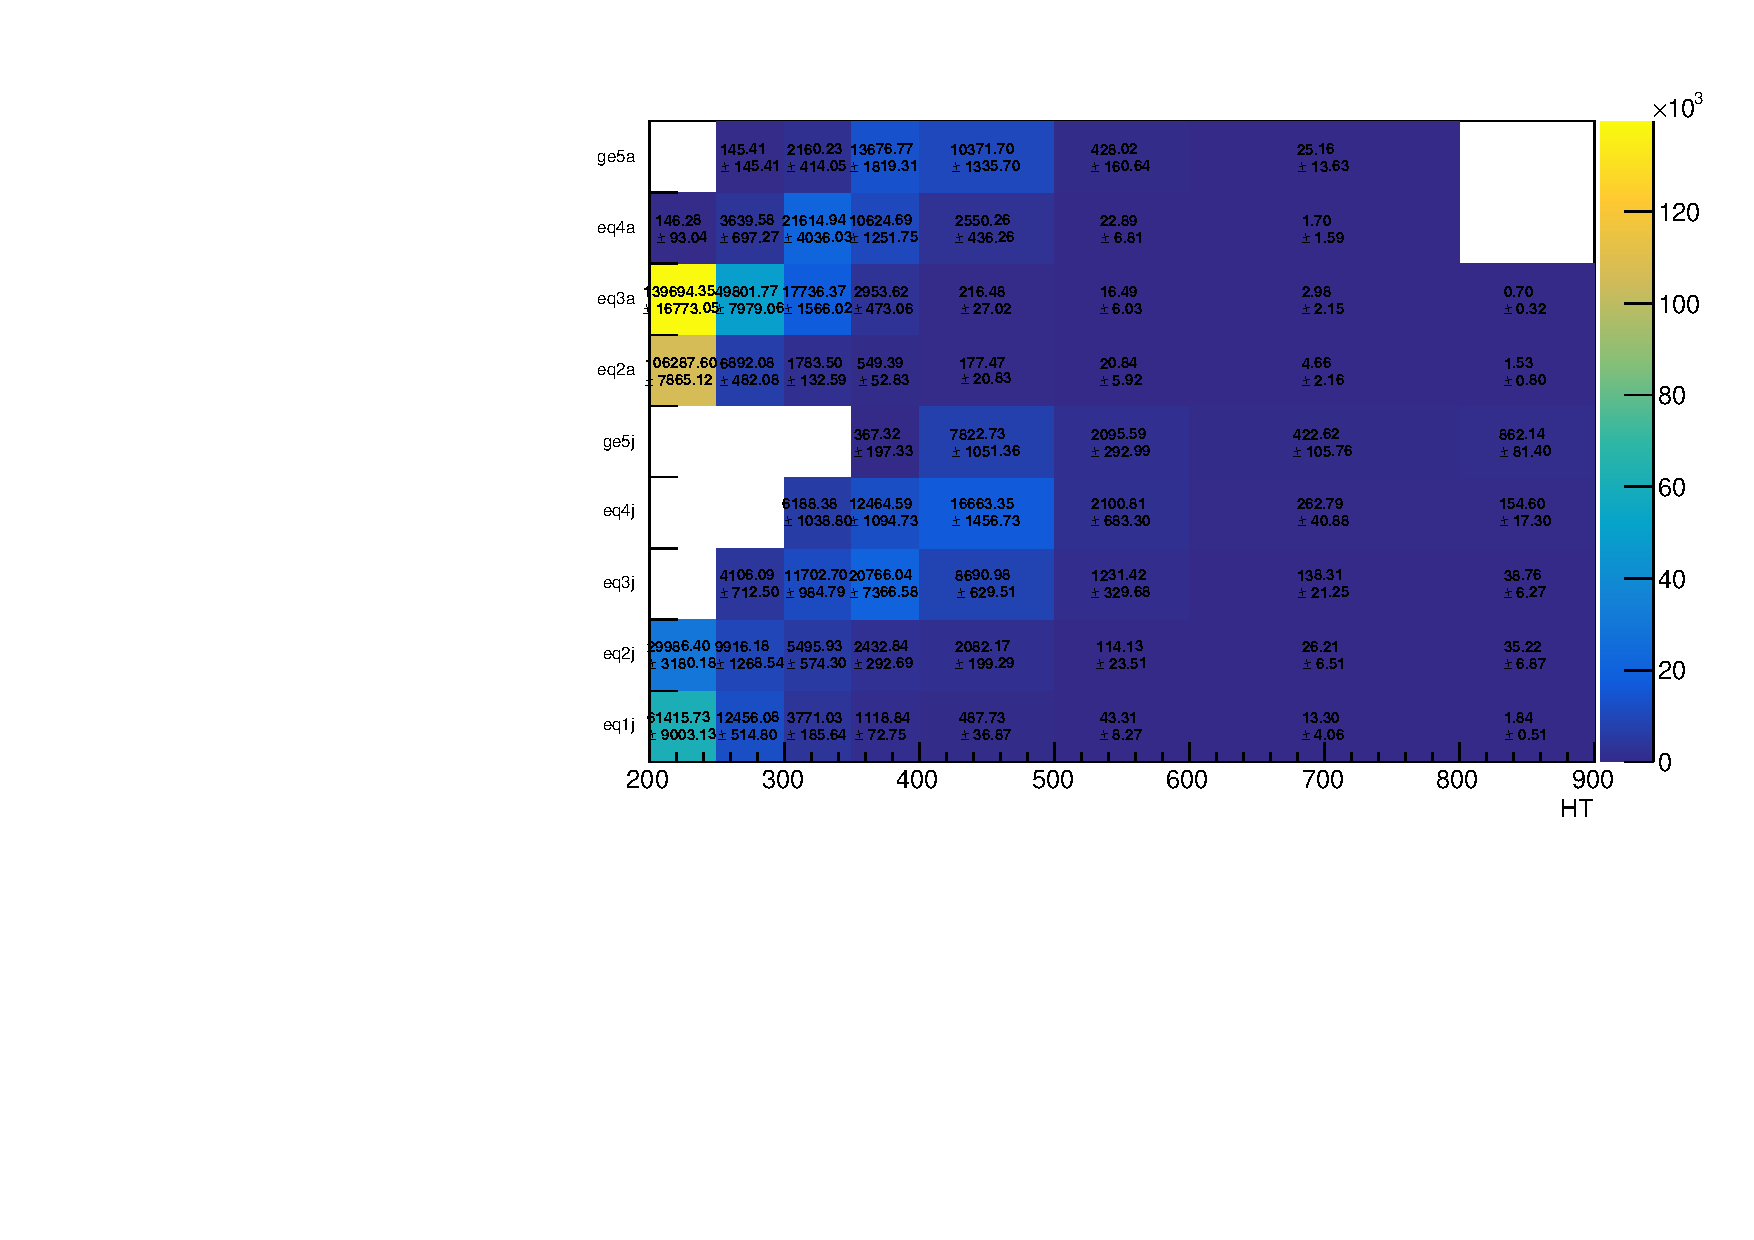
\includegraphics[width=0.5\textwidth]{figs/analysis/qcdMethod/qcdSbQCD_MC}
  } \\
  \subfloat[Ratio \rmhtmet for simulated \QCD events.\label{fig:qcd_ratio}]{
    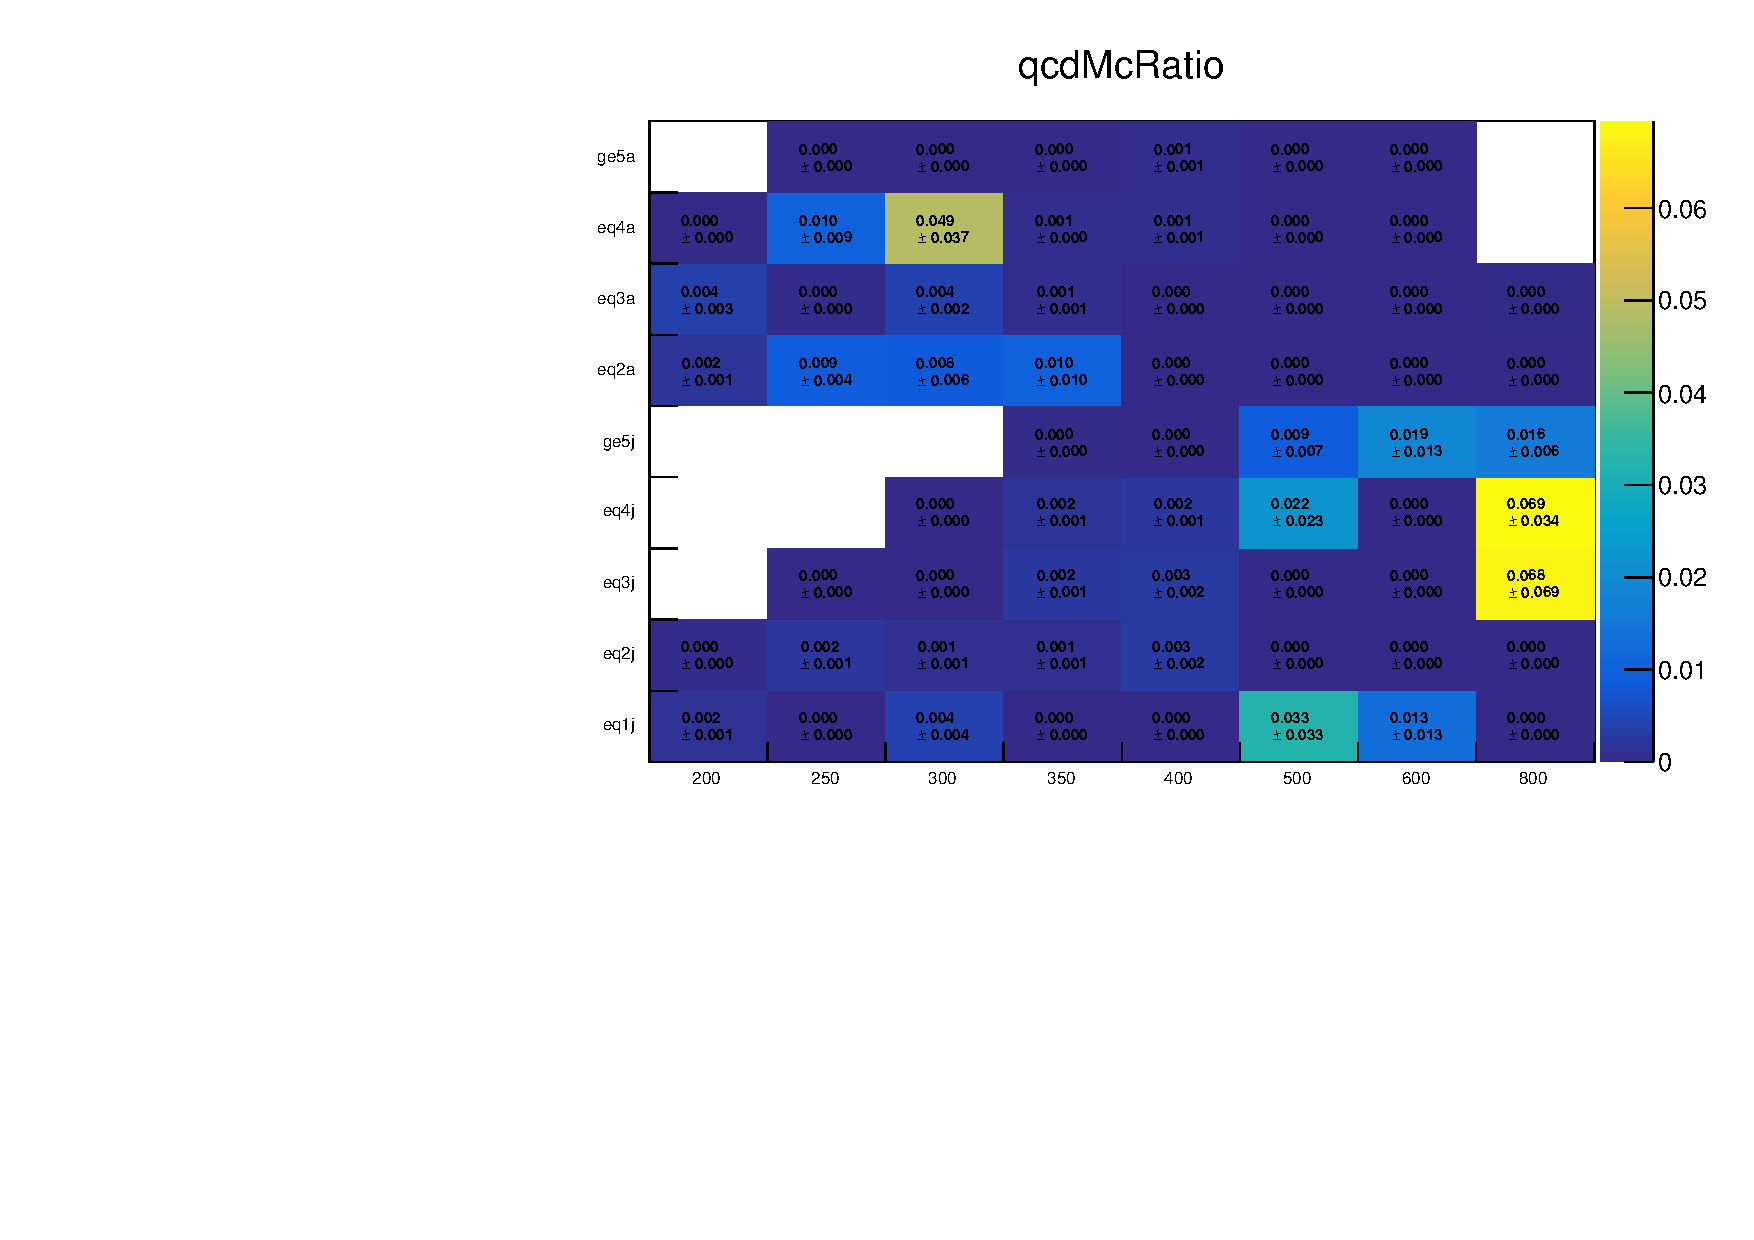
\includegraphics[width=0.5\textwidth]{figs/analysis/qcdMethod/signalQcdDivSbQcd_MC}
  } 
  \subfloat[Predicted electroweak backgrounds in the \mhtmet sideband.\label{fig:ewk_fail}]{
    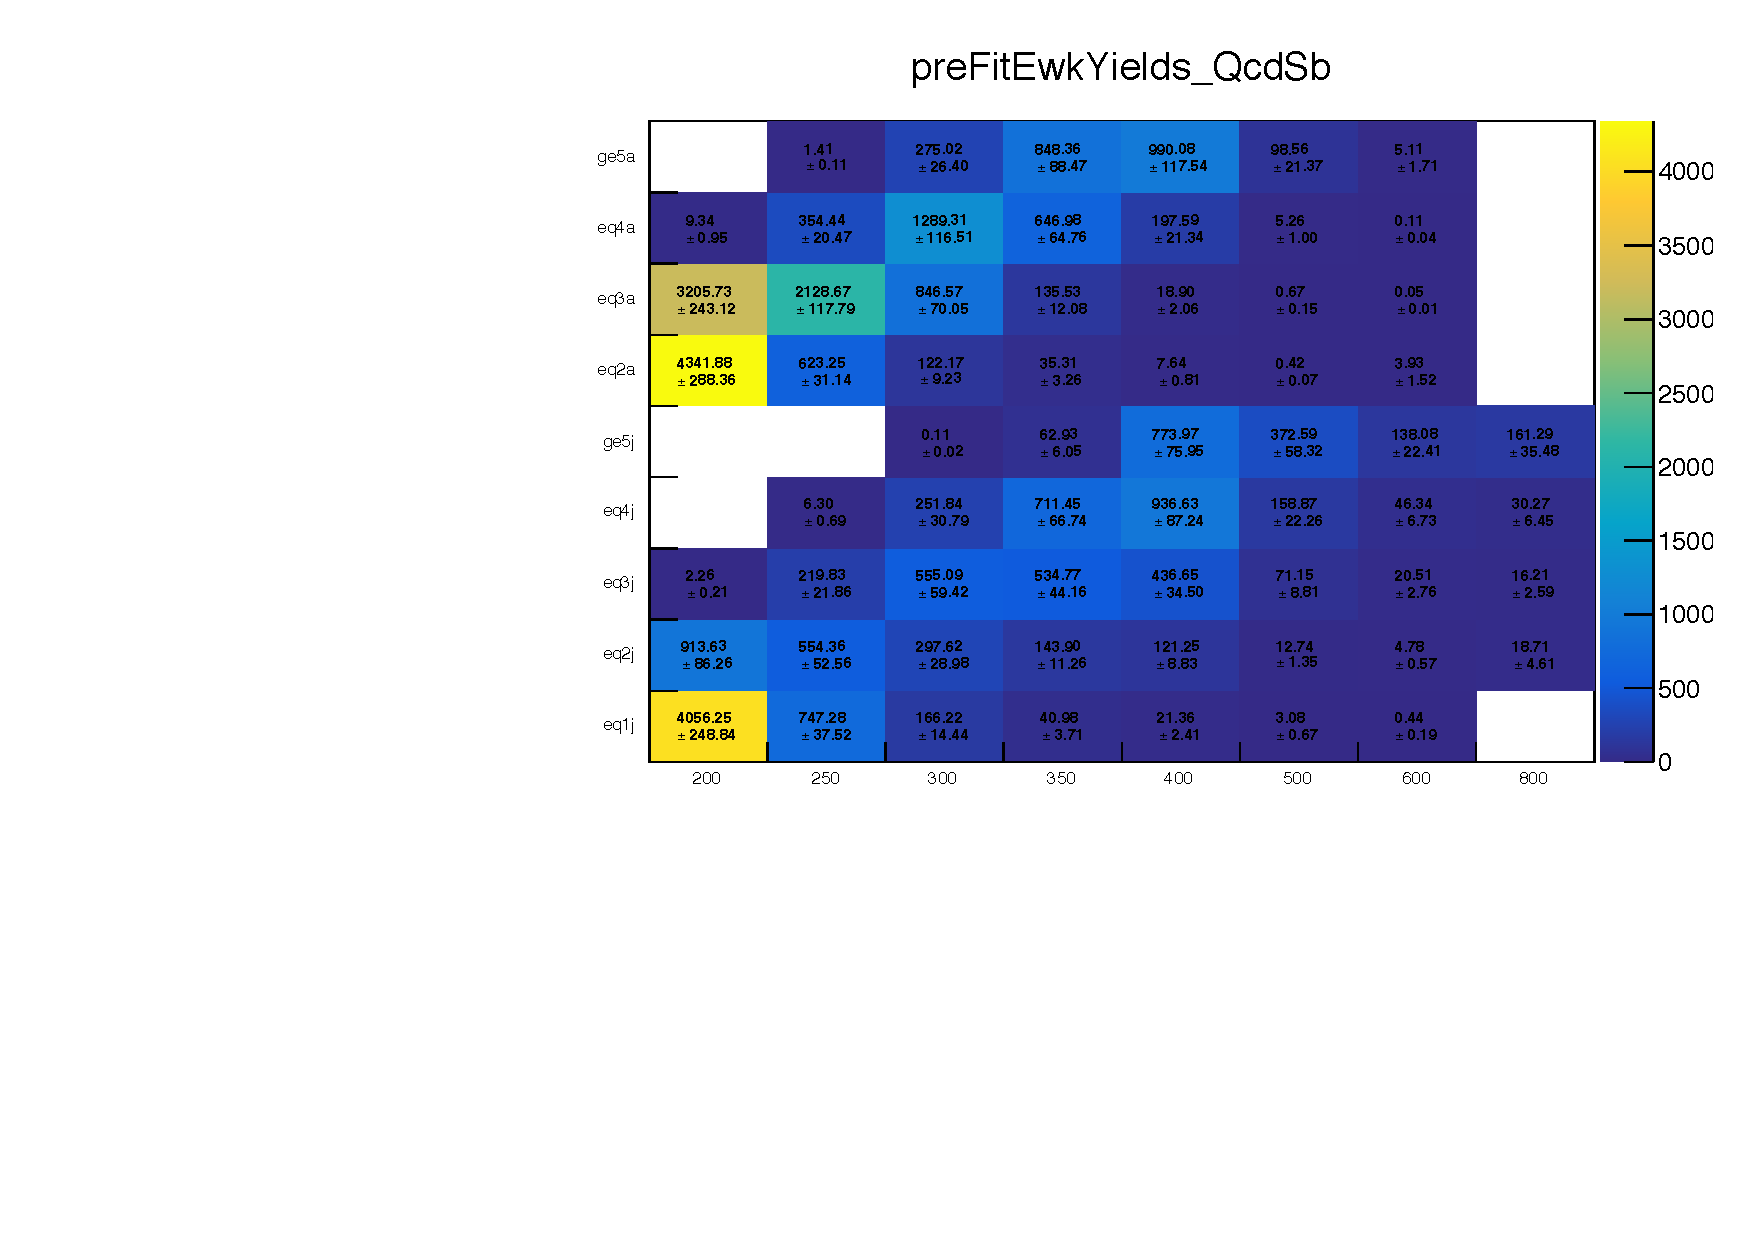
\includegraphics[width=0.5\textwidth]{figs/analysis/qcdMethod/qcdSbEwk_MC}
   %    \includegraphics[width=0.5\textwidth]{figures/qcd/v6/Ewk/SigTrig_FailMoM_NJet_vs_HT_bDPhigt0p5_Log}
  } \\
  \caption{Expected number of QCD multijet events determined from
    simulation, binned according to \njet and \scalht, that (a) satisfy
    and (b) fail the requirement $\mhtmet < 1.25$. The bins are
    labelled as described in App.~\ref{app:plotKey}. Also shown in (c)
    is the ratio \rmhtmet for QCD multijets, again determined from
    simulation. Finally, (d) shows the expected number of non-multijet
    eventse (V+jets and \ttbar, plus other residual non-multijet
    backgrounds) that fail the $\mhtmet < 1.25$ requirement, predicted
    using the \TF method and binned according to \njet and \scalht.}
  \label{fig:qcd_plots}
\end{figure}

The number of counts from \QCD multijet events satisfying and failing the
requirement $\mhtmet < 1.25$, \rmhtmet, are
summarised in Fig.~\ref{fig:qcd_pass}, \ref{fig:qcd_fail}, and
\ref{fig:qcd_ratio}. Figure~\ref{fig:ewk_fail} shows the expected
counts from non-multijet backgrounds in the \mhtmet sideband,
predicted with the \TF method.

\begin{figure}[!h]
  \centering
  \subfloat[Binned data counts in \mhtmet sideband.\label{fig:data_fail}]{
    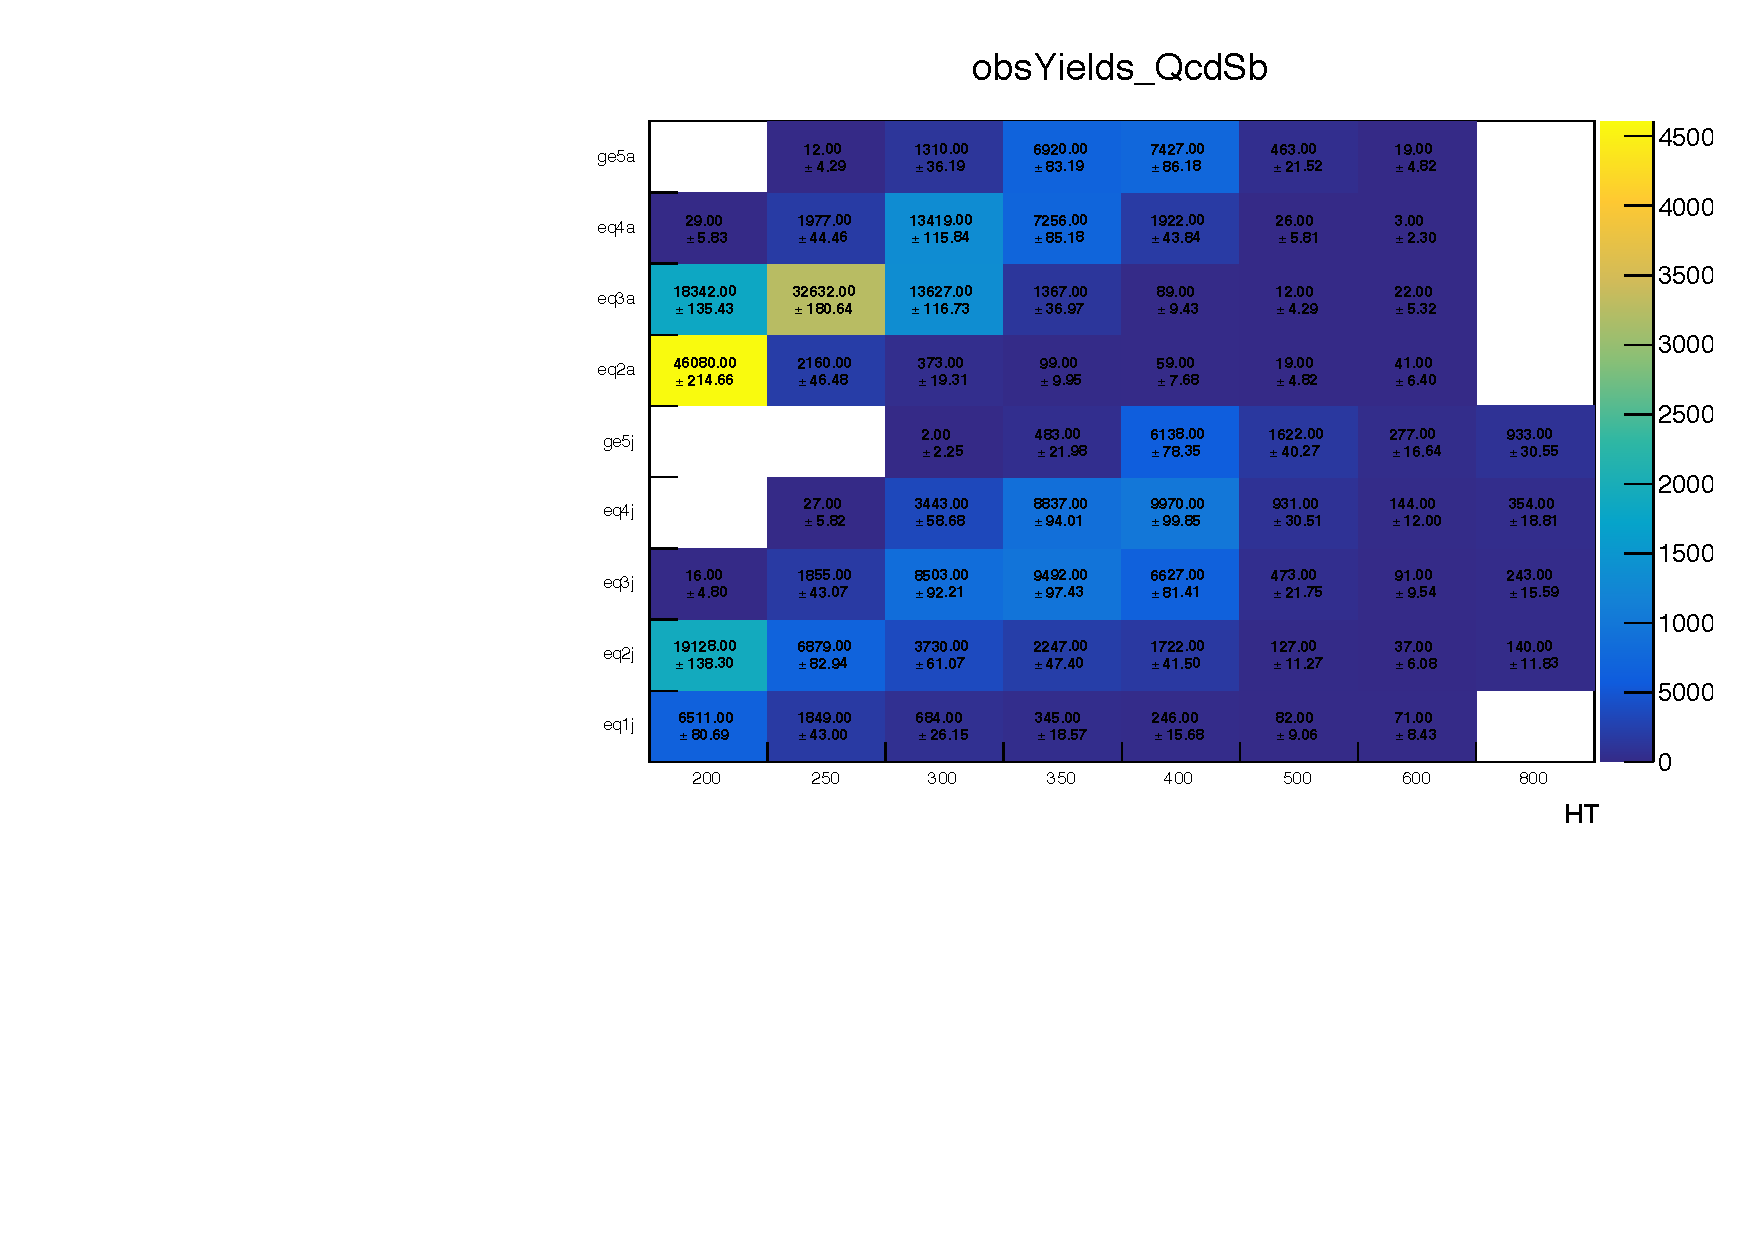
\includegraphics[width=0.5\textwidth]{figs/analysis/qcdMethod/obsYields_QcdSb}
  } 
  \subfloat[Predicted QCD counts in \mhtmet sideband.\label{fig:data_corr}]{
    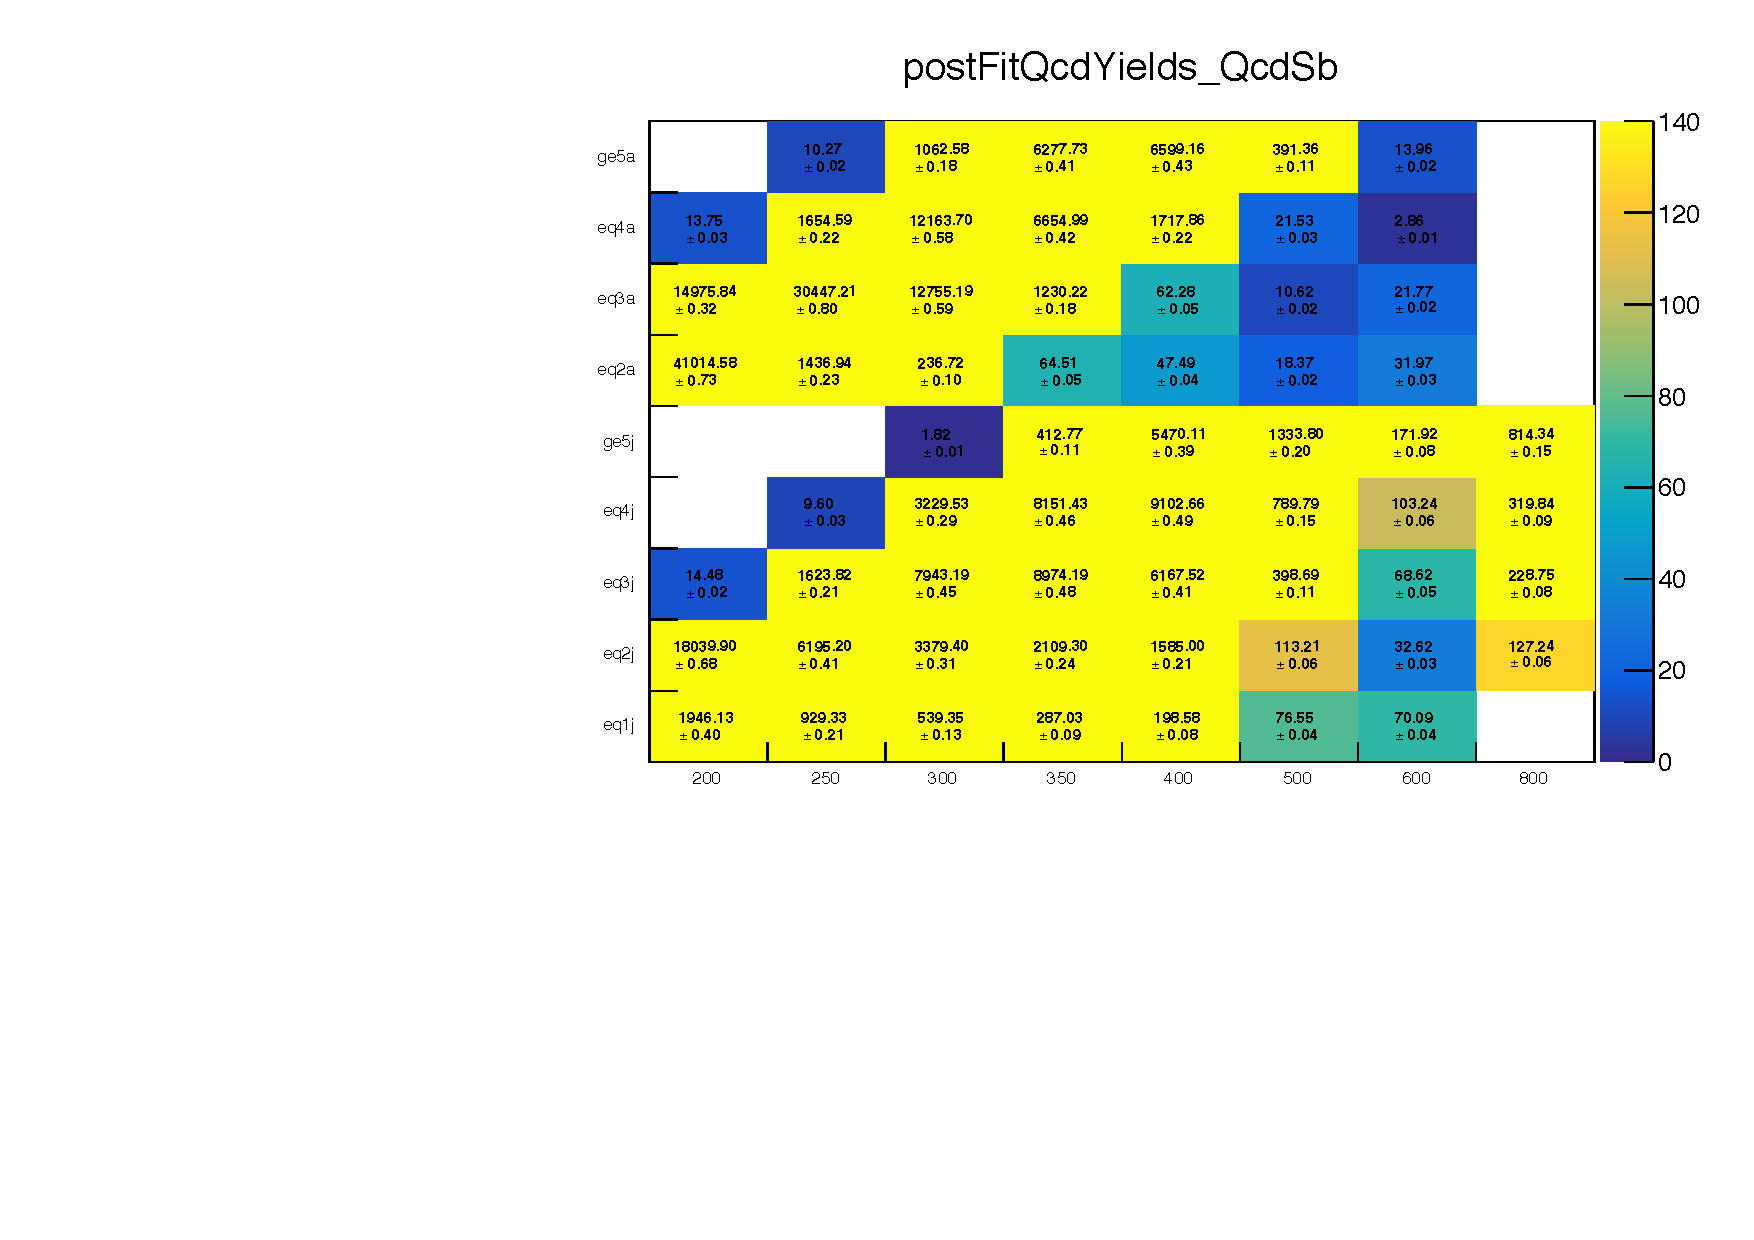
\includegraphics[width=0.5\textwidth]{figs/analysis/qcdMethod/postFitQcdYields_QcdSb}
  } \\
  \subfloat[QCD multijet predictions in the signal region.\label{fig:qcd_pred}]{
    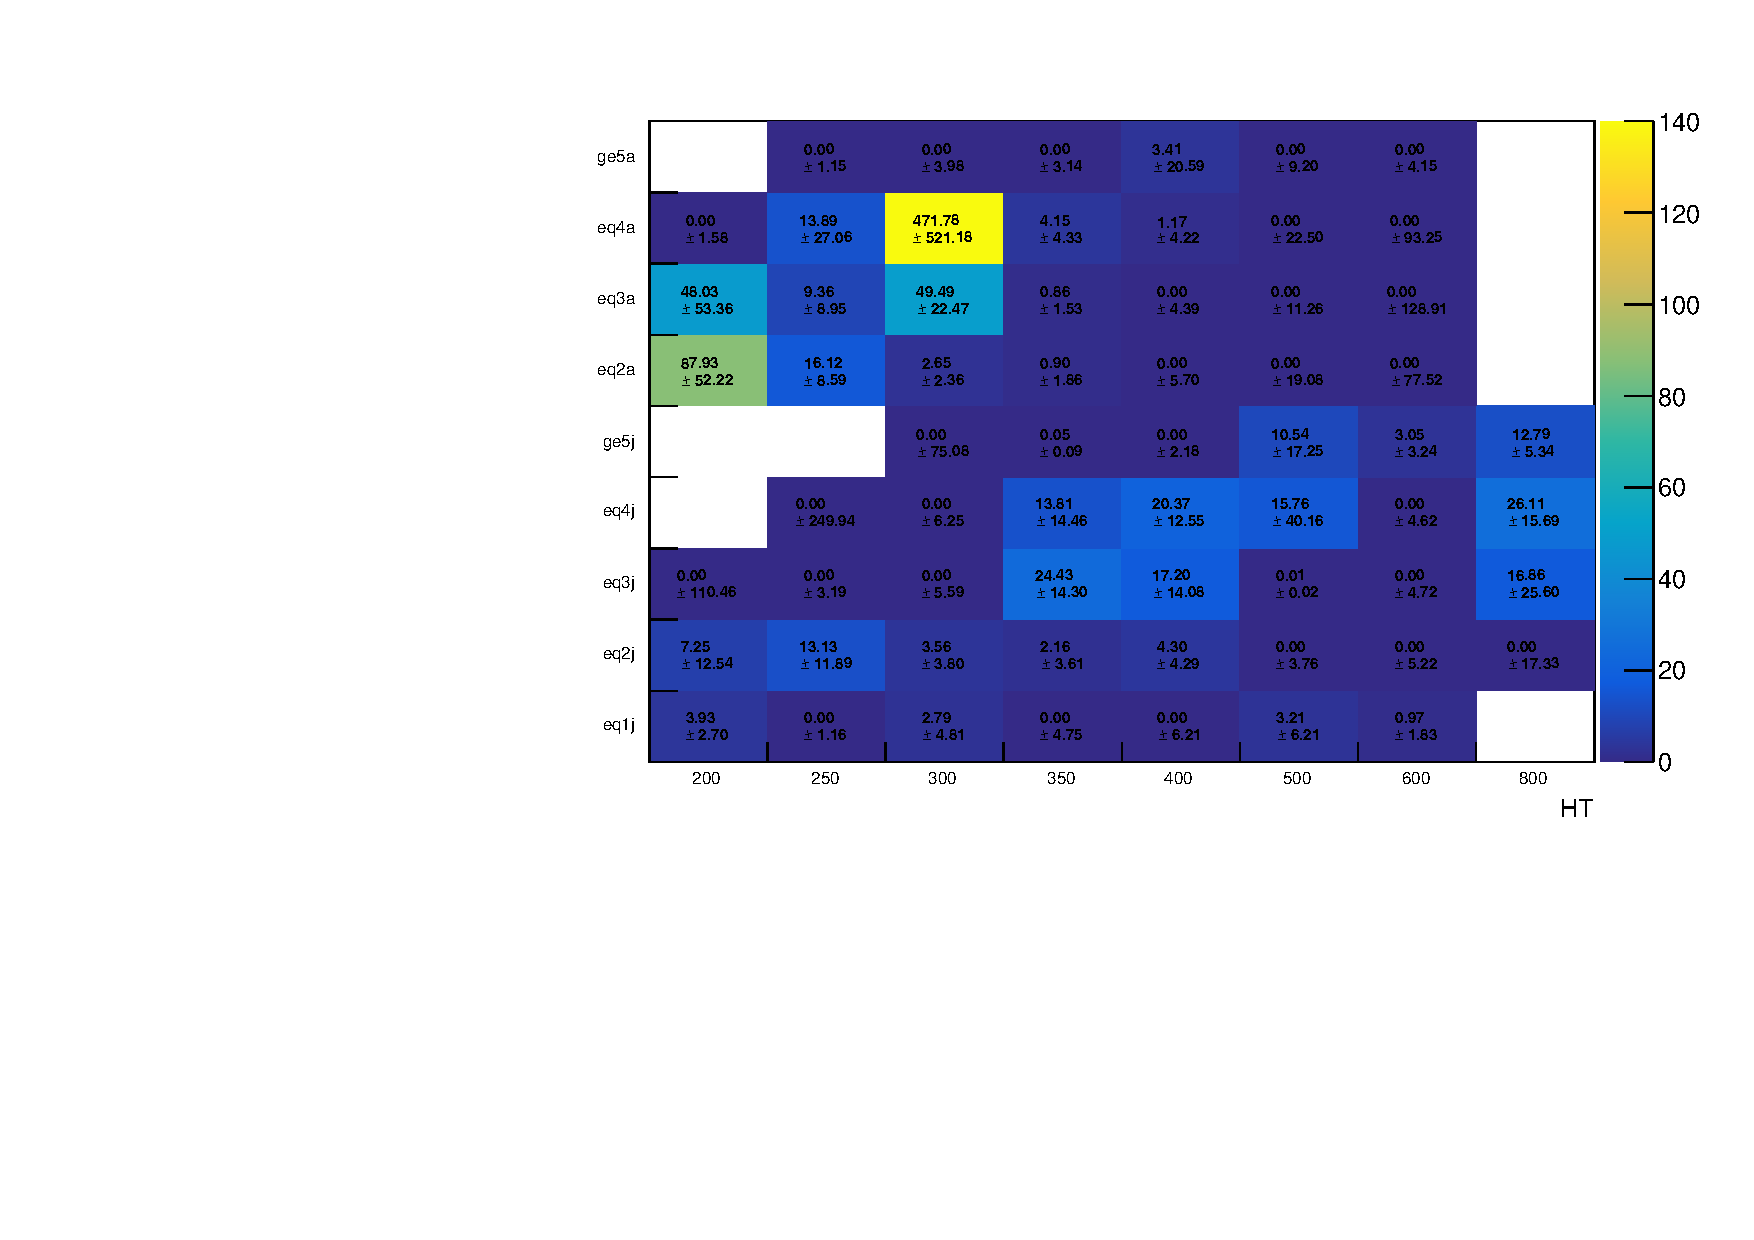
\includegraphics[width=0.5\textwidth]{figs/analysis/qcdMethod/predictedQcdYields_Signal}
  } 
  \subfloat[Ratio of predicted multijet and non-multijet yields in the
  signal region.\label{fig:qcd_ewk_ratio}]{

    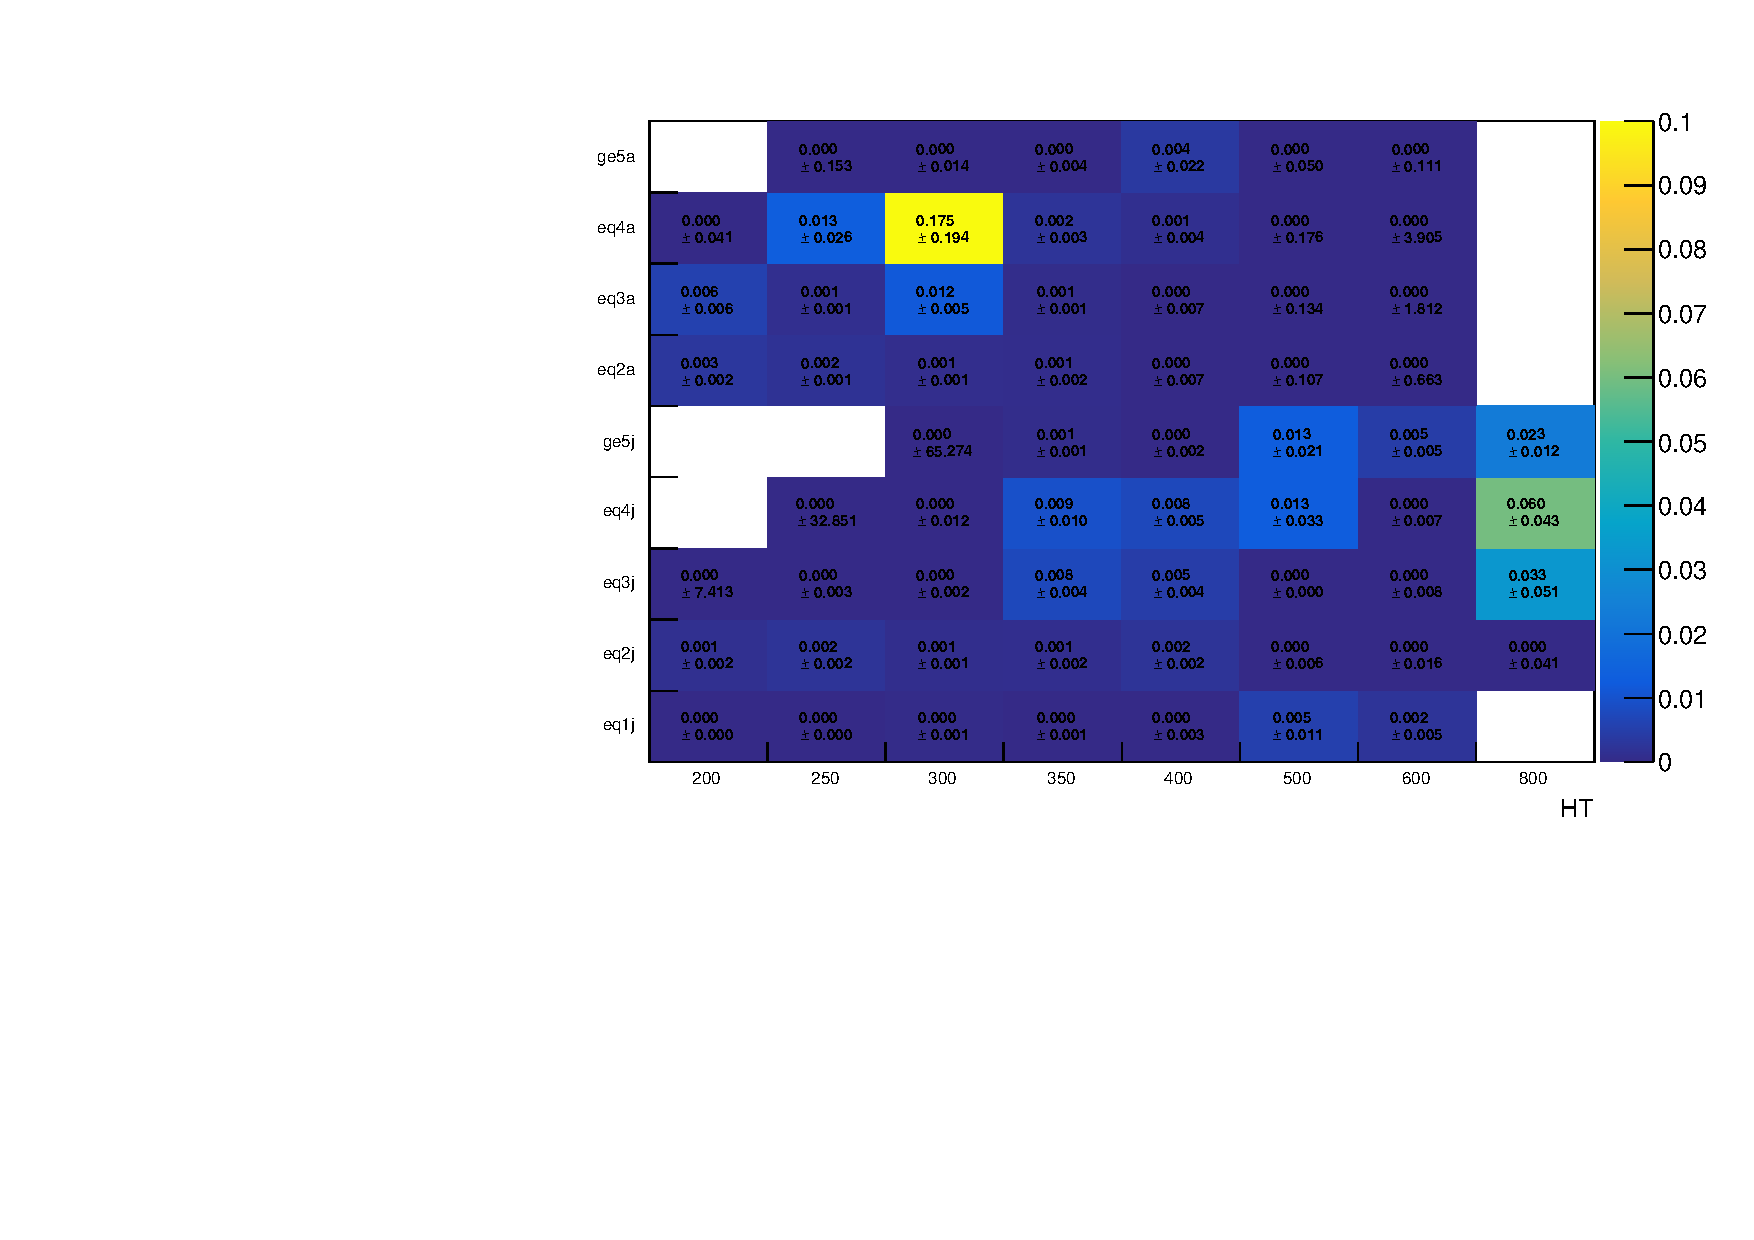
\includegraphics[width=0.5\textwidth]{figs/analysis/qcdMethod/predictedQcdDivEwk_Signal}
  } \\
  \caption{The number of events observed in the $\mhtmet>1.25$ sideband, 
    binned according to \njet and \scalht are shown in (a). The bins are
    labelled as described in App.~\ref{app:plotKey}. In
    (b) these yields are corrected by subtracting the expected
    electroweak component. Shown in
    (c) is the result of multiplying the observed multijet events predicted
    in (b) by the translation factor from the sideband to the signal
    region determined with simulation (shown in
    Fig.~\ref{fig:qcd_plots}). This gives a data driven expectation of
    the quantity of multijet background events in the signal region. 
    Finally, (d), shows the ratio of expected
    multijet background events in the signal region divided by
    non-multijet backgrounds. The multijet background is therefore
    shown to be at the percent level.}
  \label{fig:qcd_plots2}
\end{figure}

% THIS IS NOW UNNECESSARY:  
% The data counts in the \mhtmet sideband are collected with the
% \verb!HLT_HTxxx_AlphaT0pyy!  and \verb!HLT_HT800! signal triggers
% described in Sec.~\ref{sec:triggers}. Events satisfy the full signal
% region requirements plus the inverted \mhtmet requirement and are
% binned according to \njet and \scalht. 
% Any contribution from
% non-multijet backgrounds (V+jets, \ttbar, \etc) in each bin is
% estimated from simulation\footnote{In the future, the counts from
%   non-multijet backgrounds will be estimated from the muon data
%   control samples and transfer factors determined from simulation
%   (using the method described in Sec.~\ref{sec:backgroundmet}).} and
% subtracted from the data counts. Any remaining counts, $\mathcal{Q}$,
% are assumed to arise from multijet production.

Figure~\ref{fig:data_fail} shows the observed counts in the \mhtmet
sideband, and Fig.~\ref{fig:data_corr} shows the QCD counts 
in the sideband predicted by the maximum likelihood fit.
Figure~\ref{fig:qcd_pred} shows the predicted counts for the multijet
contribution in the signal region bins, which are obtained from the
products of \rmhtmet and $\mathcal{Q}$, summarised in
Figs.~\ref{fig:qcd_ratio} and \ref{fig:data_corr}. Finally,
Fig.~\ref{fig:qcd_ewk_ratio} shows the ratios of predicted multijet
counts with respect to the expected counts from the other backgrounds
with genuine \MET in the signal region, predicted with the procedure
defined in Sec.~\ref{sec:bkgdMet}.
% This allows the quantification of
% the (predicted) relative contamination from multijet events in the
% signal region bins. 
% The EWK \mht and \nb shapes derived from
% simulation are used to predict the distribution 
% of QCD events, this approach is validated in
% Sec.~\ref{sec:qcdValidation}. 

%% The predictions summarised in Fig.~\ref{fig:qcd_ewk_ratio} support the
%% expectation based on experience with 8~TeV data that the \HT-dependent
%% \alphat thresholds defined in Table~\ref{tab:sr-selections} and the
%% requirement of $\bdphi > 0.5$ are sufficient to reduce the multijet
%% contamination in all bins of the signal region to the sub-percent with
%% respect to the total non-multijet background. With this level of
%% suppression, it is expected that the uncertainty associated with the
%% residual multijet contamination to be sub-dominant with respect to,
%% and fully absorbed by, the systematic uncertainties on the non-multijet
%% backgrounds, which are expected to be at the level of $\sim$10\% or
%% larger. 

The predictions summarised in Fig.~\ref{fig:qcd_ewk_ratio} show that 
the \HT-dependent \alphat thresholds defined in Table~\ref{tab:atCut} 
and the requirement of $\bdphi > 0.5$ suppress the \QCD multijet
contamination in all bins of the signal region to percent-level or smaller with
respect to the total non-multijet background. These predicted multijet events are 
included as a background contribution to the likelihood model
described in Sec~\ref{sec:likelihood}.

As the prediction of \QCD in the signal region is carried out
inclusively over \nb and \mht, the \QCD shapes for these variables are
taken from the non-multijet simulation and normalised to the \QCD counts. A
lack of statistics in the \QCD simulation led to the adoption of this approach.
Within uncertainties, the level of
agreement is deemed acceptable given the small total \QCD contribution to the
signal region.

\subsection{Validation} 
\label{sec:qcdVal}

Despite using a predominantly data-driven method, the prediction of
the \QCD contamination relies on the ratio of \QCD counts, \rmhtmet,
that is derived with simulation. This ratio is validated with data in
a \QCD enriched sideband, where full signal region selection is used
other than an inversion of the \bdphi cut to $\bdphi<0.5$. In this
sideband a data driven estimation of the \QCD counts is carried out in
two regions, the \bdphi sideband with \mhtmet values less than 1.25
and the double sideband with
values greater than 1.25. These predictions are again made with a maximum
likelihood fit, analogous to that described in
Sec.~\ref{sec:qcdMethod}. This fit estimates the counts in the
non-multijet backgrounds with \mj, \mmj and \gj
control regions and all relevant systematic errors. The
remaining data counts in each sideband are then attributed to \QCD.
With this estimation of \QCD it is possible to derive a data driven
ratio of \QCD counts with $\mhtmet<1.25$ and those with $\mhtmet>1.25$,
$\rmhtmet_{\bdphi<0.5}^{data}$. By taking \MC counts in the \bdphi
sideband it is also possible to calculate the \mhtmet simulation
ratio, $\rmhtmet_{\bdphi<0.5}$. 

To validate the ratio \rmhtmet, it is assumed that if the simulation of
the ratio in the \bdphi sideband agrees with that derived from data,
the simulated ratio that is not in the sideband is valid. Any
disagreement is covered by a systematic error on the signal region QCD
prediction. The ratio of $\rmhtmet_{\bdphi<0.5}$ and
$\rmhtmet_{\bdphi<0.5}^{data}$ in \scalht and \njet bins is shown in
Fig.~\ref{fig:RR_qcd}. Bins in which there are insufficient statistics
in data or simulation to make the calculation are left out. This plot
illustrates that a fully correlated systematic of 100\% taken on the
predicted \QCD contamination in the signal region should cover any
disagreement between simulation and data.

\begin{figure}[h!]
  \begin{center}        
    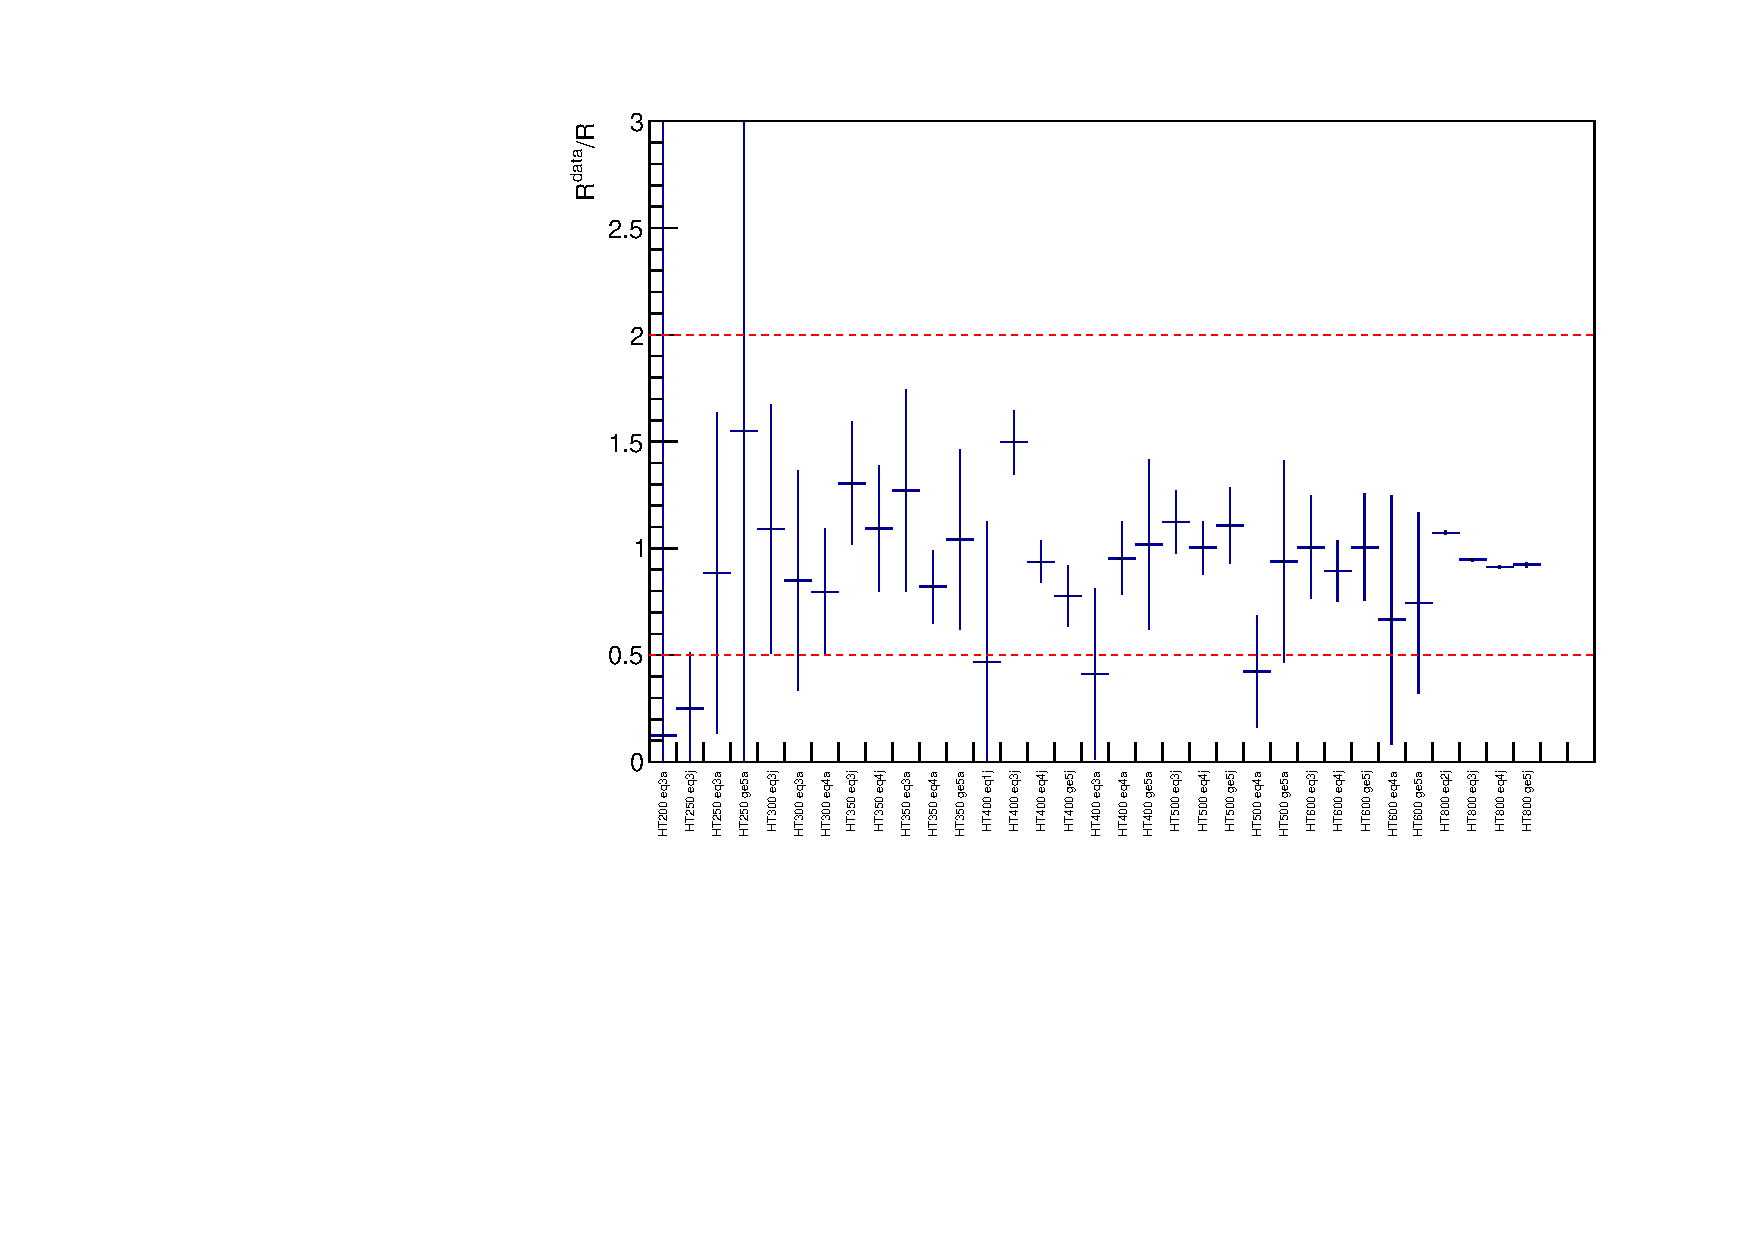
\includegraphics[width=\textwidth]{figs/analysis/qcdMethod/doubleQcdSbSrRatio1D}
    \caption{ Ratio of the measurement of \rmhtmet, the pass/fail
    ratio for the \mhtmet selection, from data and Monte Carlo in the
    $\bdphi < 0.5$ sideband in (\scalht, \njet) bins. Dotted red lines
    demonstrate that disagreement is covered by a 100\% systematic
    uncertainty on the ratio. The bins are
    labelled as described in App.~\ref{app:plotKey}.}
    \label{fig:RR_qcd}
  \end{center} 
\end{figure}

%\subsection{The \MHT and \nb dimensions}

% explain how it's implemented?
% The
% \QCD multijet contamination is included as a
% fraction of the other \SM backgrounds with genuine \MET, that are
% determined with the \TF method described in Sec.~\ref{}. It is typically a negligible
% contribution and is added to the total \SM background.

% To validate it, the simulated \mht distributions for the QCD and EWK
% processes in the signal region are divided. This is shown in
% Figs.~\ref{fig:asym_qcd_validation}-\ref{fig:asym_qcd_validation}.  As
% the normalisation is carried out independently, a flat distribution of
% the ratio is enough for validation. 


%%%%%%%%%%%%%%%%%%%%
\section{Systematic uncertainties} % day 5
\label{sec:systematics}

After defining data driven methods for estimating the \SM backgrounds
in the analysis, it is necessary to take account of all sources of
systematic uncertainties on these background predictions. In this
section the sources of systematic uncertainty in the analysis are
outlined with the different methods used for estimating them.  

Due to the exceptional treatment of the \MHT dimension when carrying
out background estimation, the systematics are split into two types.
There are those that affect the total number of events in each
(\HT,\nj,\nb) bin (integrating over \MHT), which are described in
Sections~\ref{sec:simUnc} and~\ref{sec:closureTests}. Most of these
systematics are treated as uncertainties on the \TFs used to predict
the \SM backgrounds with genuine \MET. There is also one other
systematic uncertainty added to take account of uncertainties in the
\QCD multijet background prediction, described in
Sec.~\ref{sec:qcdVal}. Additionally, systematic uncertainties are
included that encode the limited knowledge on how the events
distribute in the \mht dimension, described in Sec.~\ref{sec:systMht}.

There are two approaches that are used to derive uncertainties
from different sources. There are uncertainties associated with the
correction factors that are applied to the simulation, which allows
the systematic uncertainties to be derived by varying the simulation (Sec.~\ref{sec:sfs}).
However, these sort of systematics only encode known and simulated
sources of systematic uncertainty. To be able to account of unknown
sources, additional data-driven uncertainties are derived with the
use of the control samples (Sec.~\ref{sec:closureTests}). After their
descriptions below, a summary of the all the uncertainties is given in
Tab.~\ref{tab:systs}.

\subsection{Uncertainties derived from simulation}
\label{sec:simUnc}

A set of corrections are applied to simulation that are described in
Sec.~\ref{sec:simEvents}. There is an uncertainty associated with each
of these corrections, based on the way in which they are derived and
uncertainties in any theoretical calculations that may be relevant.
These uncertainties are propagated to each of the \TFs which are of
interest for the background prediction, namely: $\mj \rightarrow
(\znunu)$, $\mmj \rightarrow (\znunu)$, $\gj \rightarrow (\znunu)$ and
$\mj \rightarrow \mathrm{\ttbar+W}$. 
% Due to the fact that the control
% regions and signal region are finely binned in the same way, the
% systematics caused by t
% The binning of the analysis is chosen in order to minimise the impact of 
% these systematic sources, which are expected to be sub-dominant.
% However, they are propagated to the final results, taking into
% account correlations and bin migration effects.


\subsubsection*{Jet energy scale}
\label{sec:tfSyst_jec}
The effect of varying the jet energy corrections (JECs) by their uncertainty
in the \mj and \mmj control regions on the \TFs is investigated.  As
the \scalht and jet multiplicity binning is mirrored in signal and
control regions, the effect of jet energy scale on the \TFs
is expected to be small.  However, the jet energy scale can still have
an effect due to jets moving in and out acceptance (above and below
$40\gev$). The relative change in the \TFs is presented as
a function of \scalht and jet category in
Fig.~\ref{fig:tfSyst_jec_muToZinv}-\ref{fig:tfSyst_jec_muToTtw}. These
plots show the change in \TFs for the \mj, \mmj and \gj control
samples as they are used to predict the \znunu and the W+\ttbar
backgrounds. The plots for the other sources of systematics can be
found in the Appendix~\ref{app:tfSysts}. The
changes are typically in the range of 1-15\%.

\begin{figure}[!h]
  \centering
  \subfloat[JEC up variation]{
    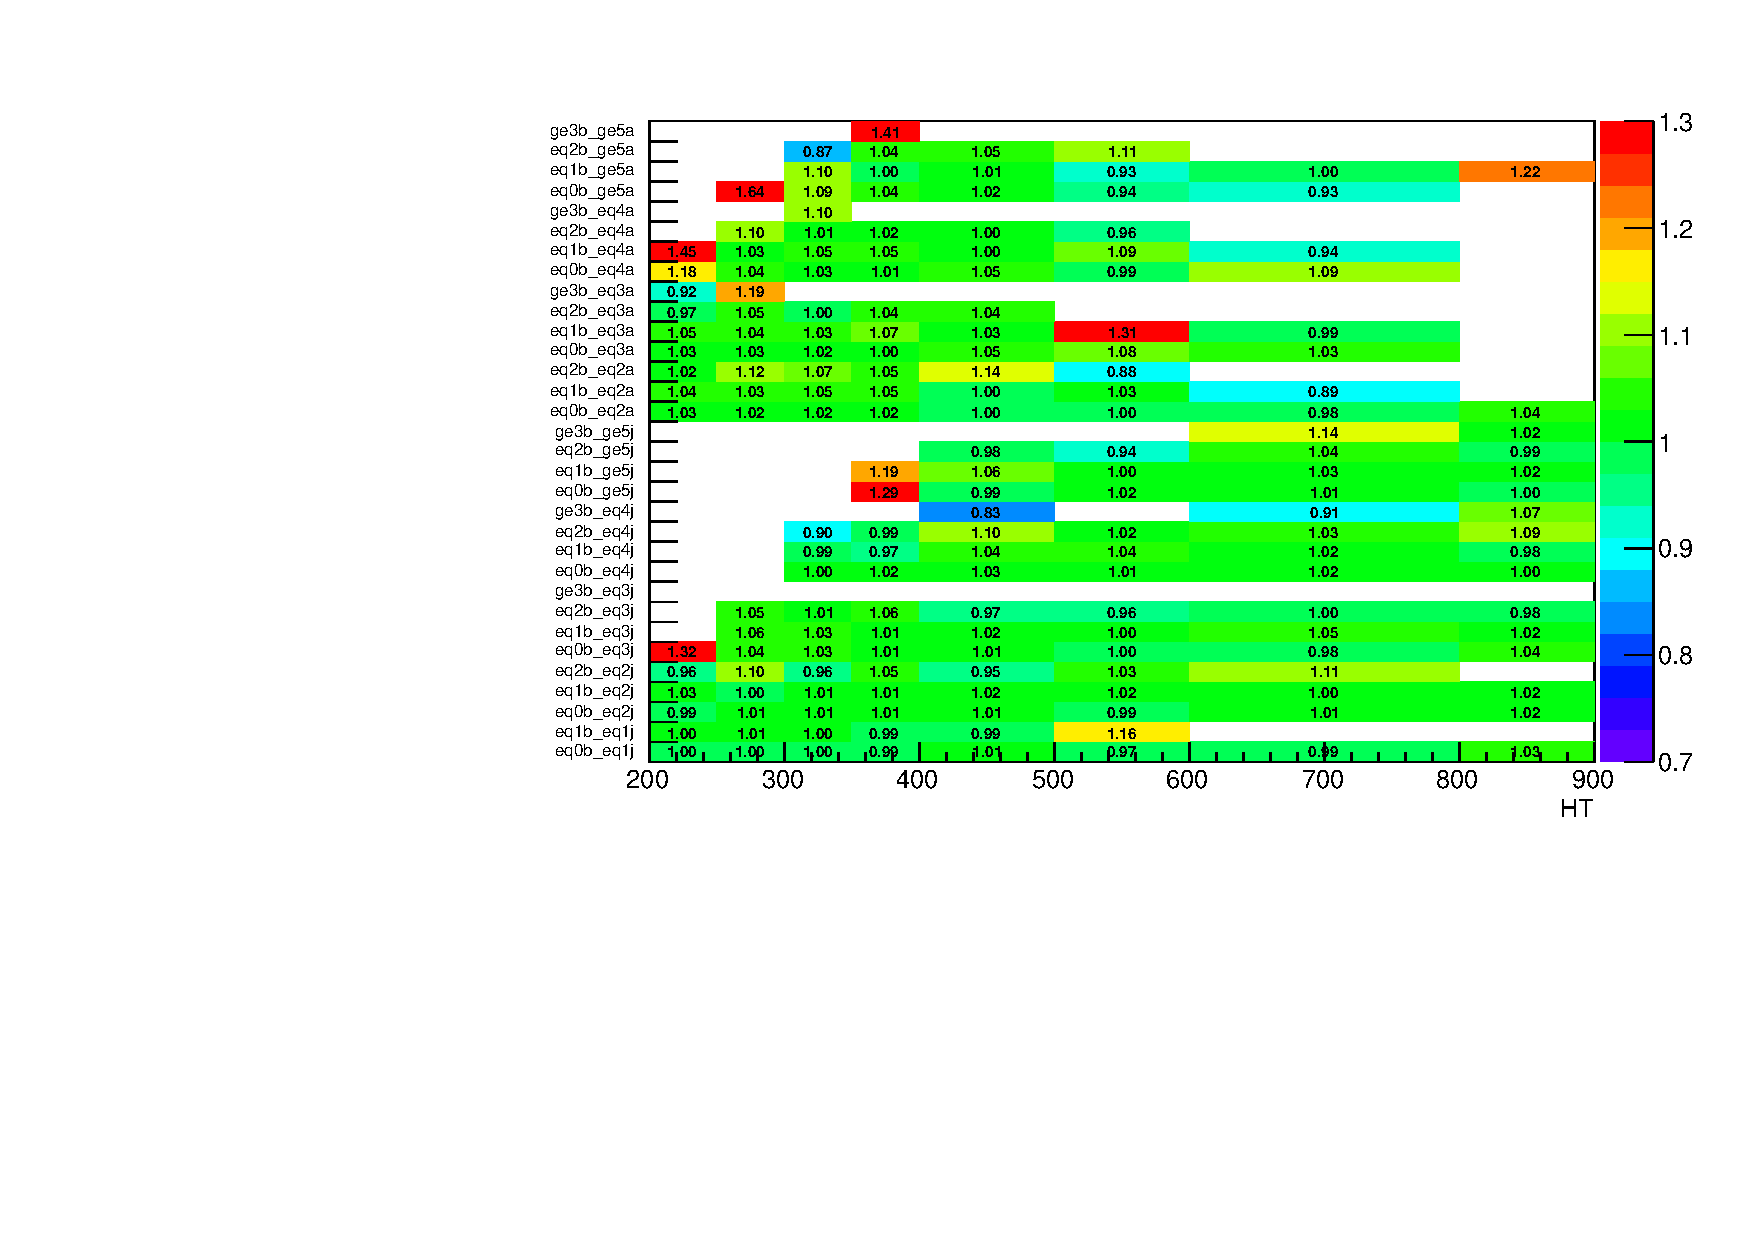
\includegraphics[width=0.5\textwidth]{figs/analysis/systsTf/Zinv/mu/ratiotfh_ht_mht_alljecWeight_Up.pdf}
  } ~~
  \subfloat[JEC down variation]{
    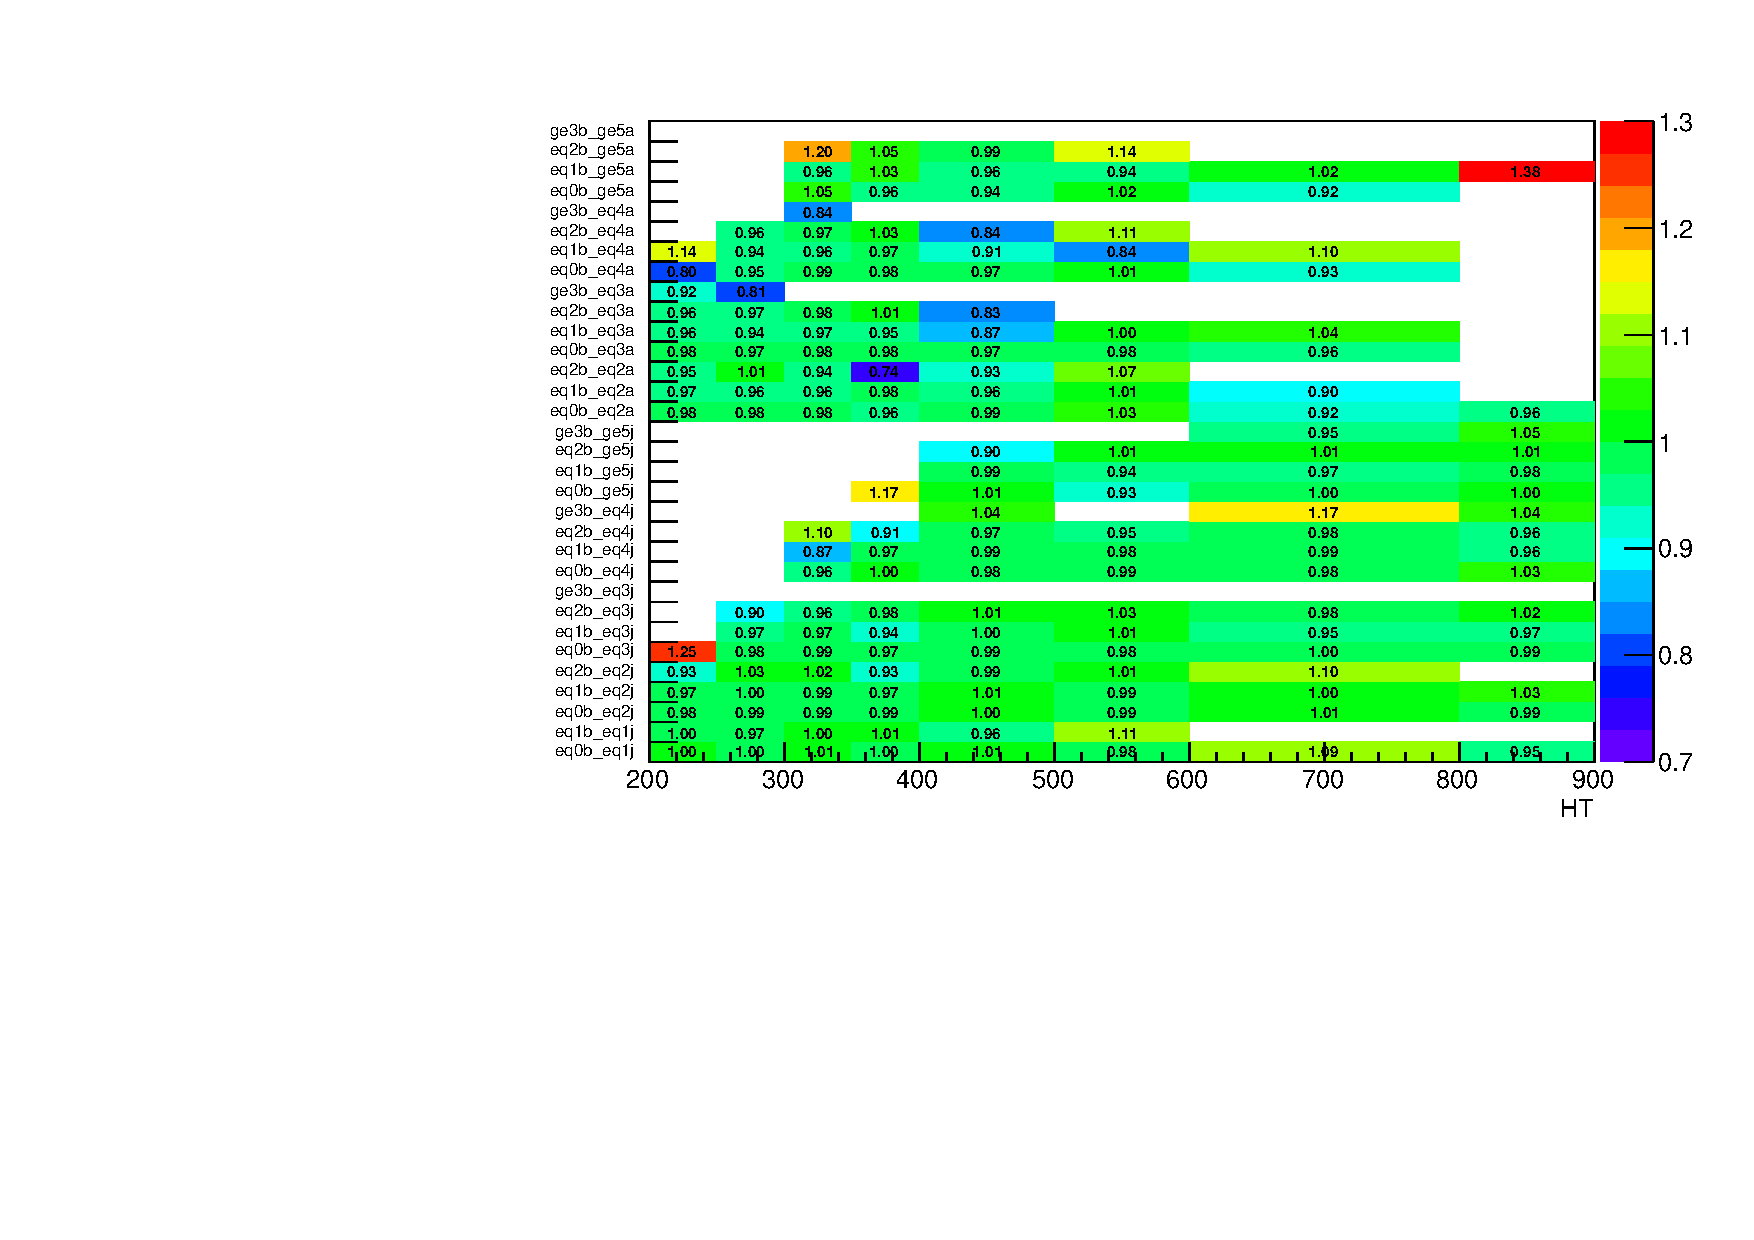
\includegraphics[width=0.5\textwidth]{figs/analysis/systsTf/Zinv/mu/ratiotfh_ht_mht_alljecWeight_Down.pdf}
  }\\

  \caption{\label{fig:tfSyst_jec_muToZinv} The relative change in the
  $\mj \rightarrow (\znunu)$ transfer
  factors when varying JEC in MC within its uncertainties, as a
  function of \scalht (GeV) and jet category.
  Variations corresponding to $+1\sigma$ ($-1\sigma$) are shown in the left (right) figure. The bins are
  labelled as described in App.~\ref{app:plotKey}.
  }
\end{figure}

\begin{figure}[!h]
  \centering
  \subfloat[JEC up variation]{
    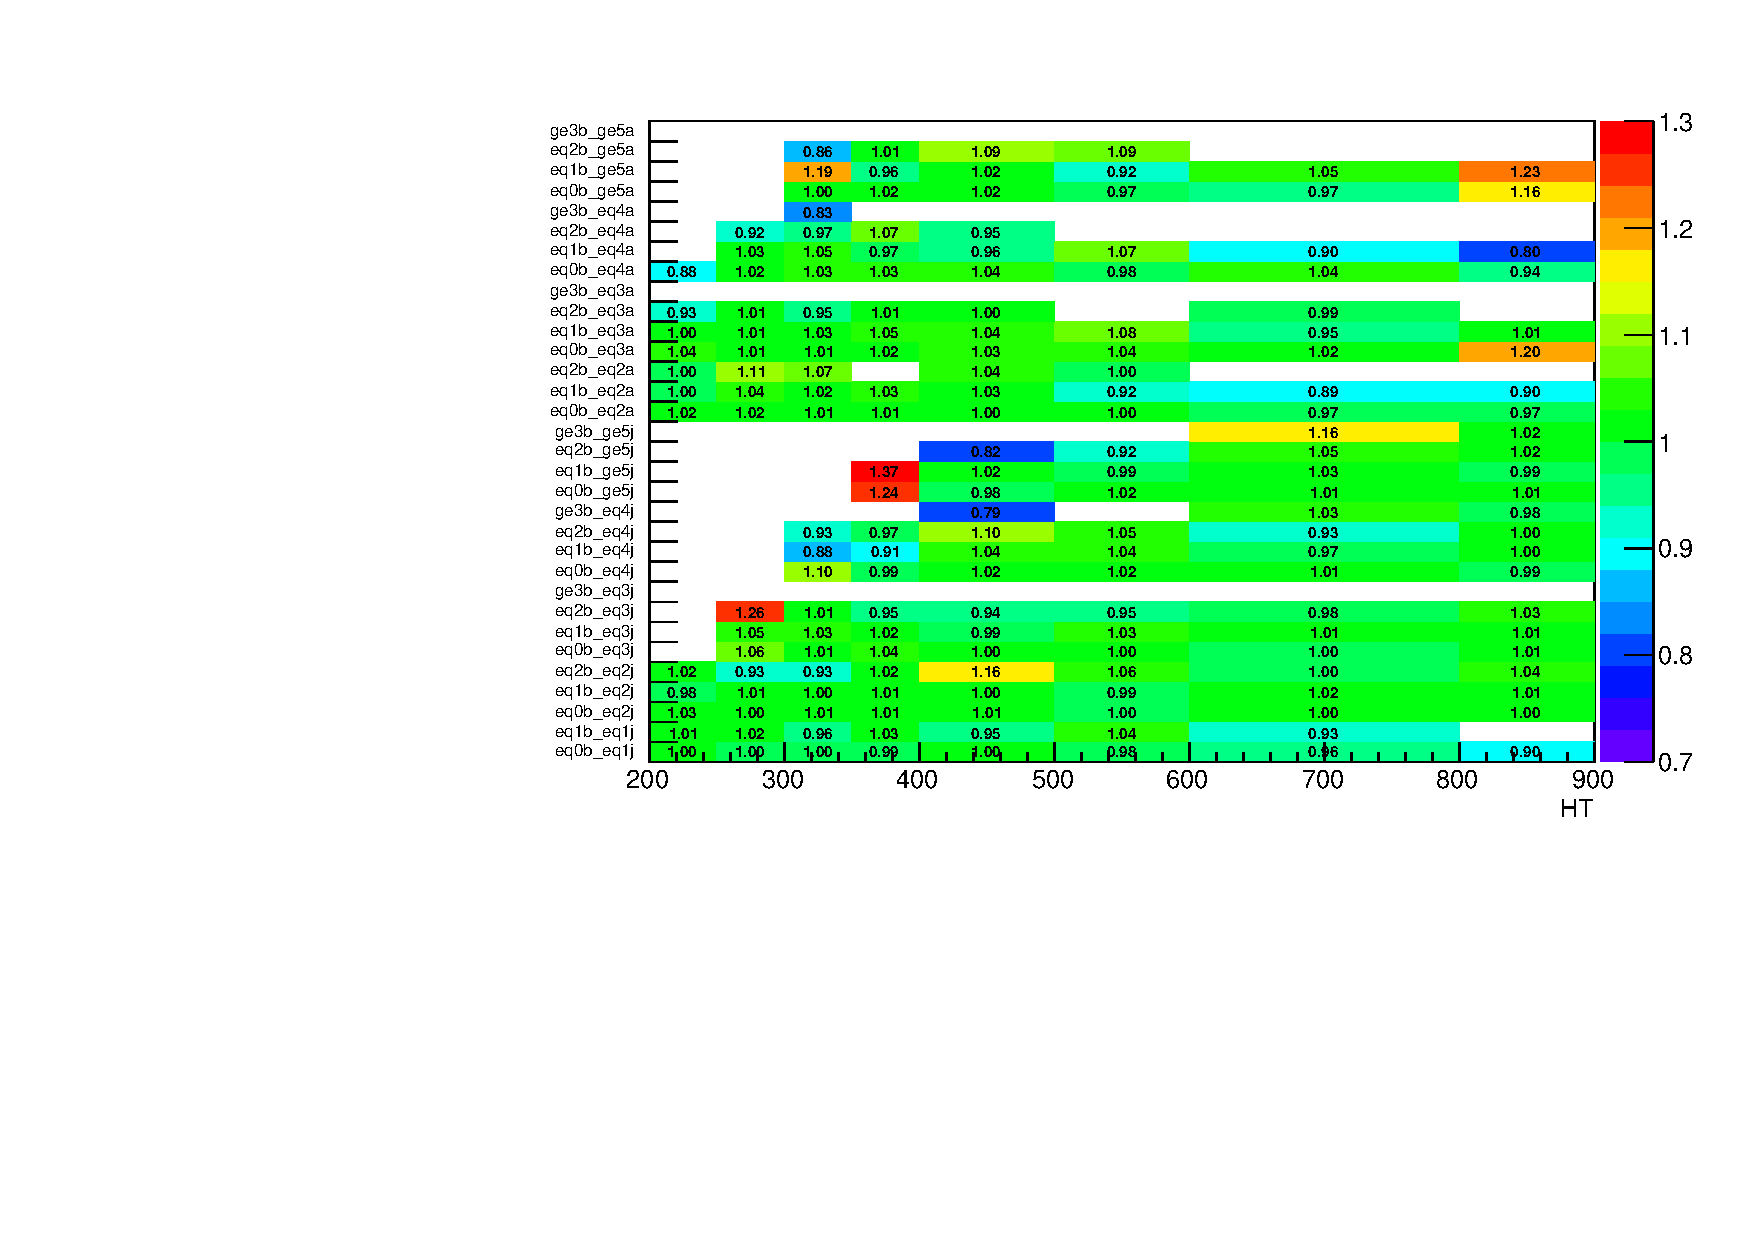
\includegraphics[width=0.5\textwidth]{figs/analysis/systsTf/Zinv/mumu/ratiotfh_ht_mht_alljecWeight_Up.pdf}
  } ~~
  \subfloat[JEC down variation]{
    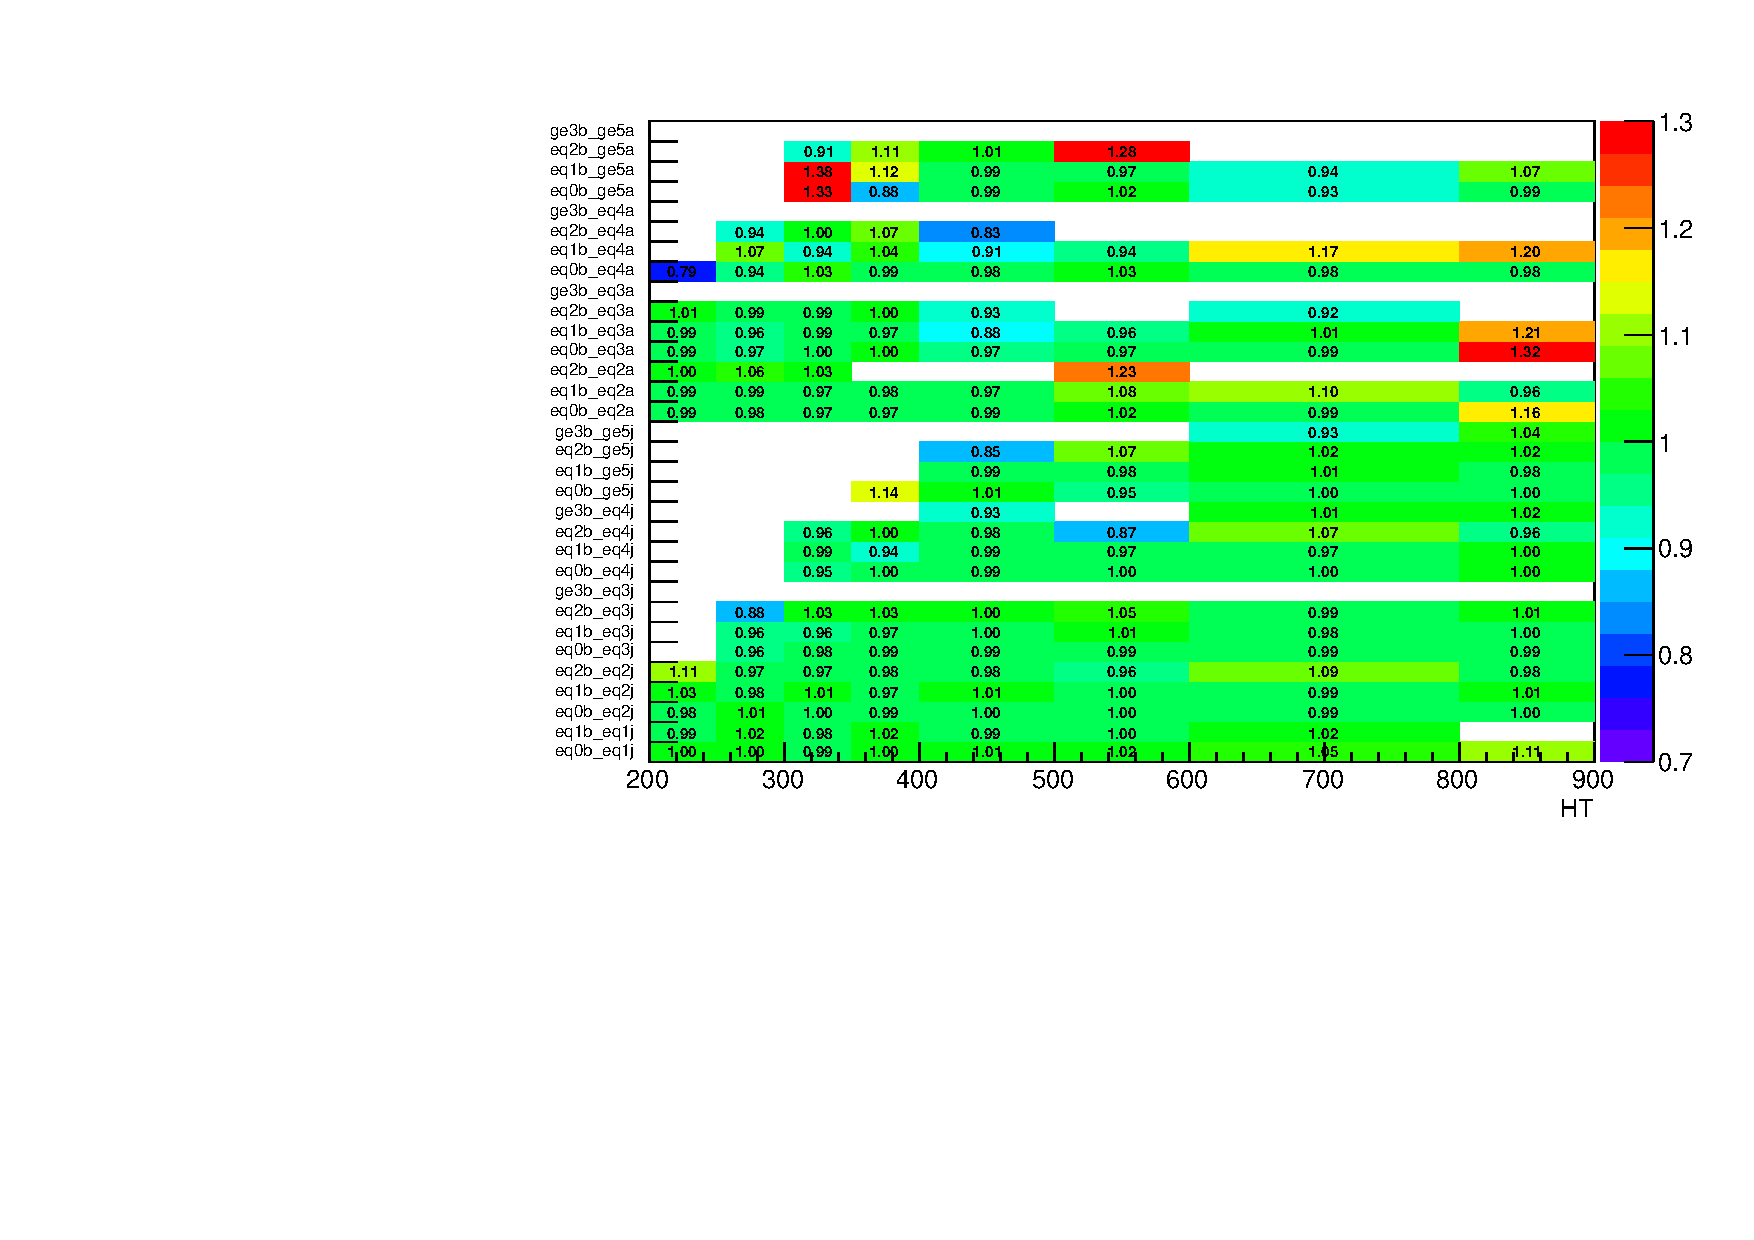
\includegraphics[width=0.5\textwidth]{figs/analysis/systsTf/Zinv/mumu/ratiotfh_ht_mht_alljecWeight_Down.pdf}
  }\\

  \caption{\label{fig:tfSyst_jec_mumuToZinv} The relative change in
  the $\mmj \rightarrow (\znunu)$ transfer
  factors when varying JEC in MC within its uncertainties, as a function of \scalht (GeV) and jet category. 
  Variations corresponding to $+1\sigma$ ($-1\sigma$) are shown in the left (right) figure. The bins are
    labelled as described in App.~\ref{app:plotKey}.
  }
\end{figure}

\begin{figure}[!h]
  \centering
  \subfloat[JEC up variation]{
    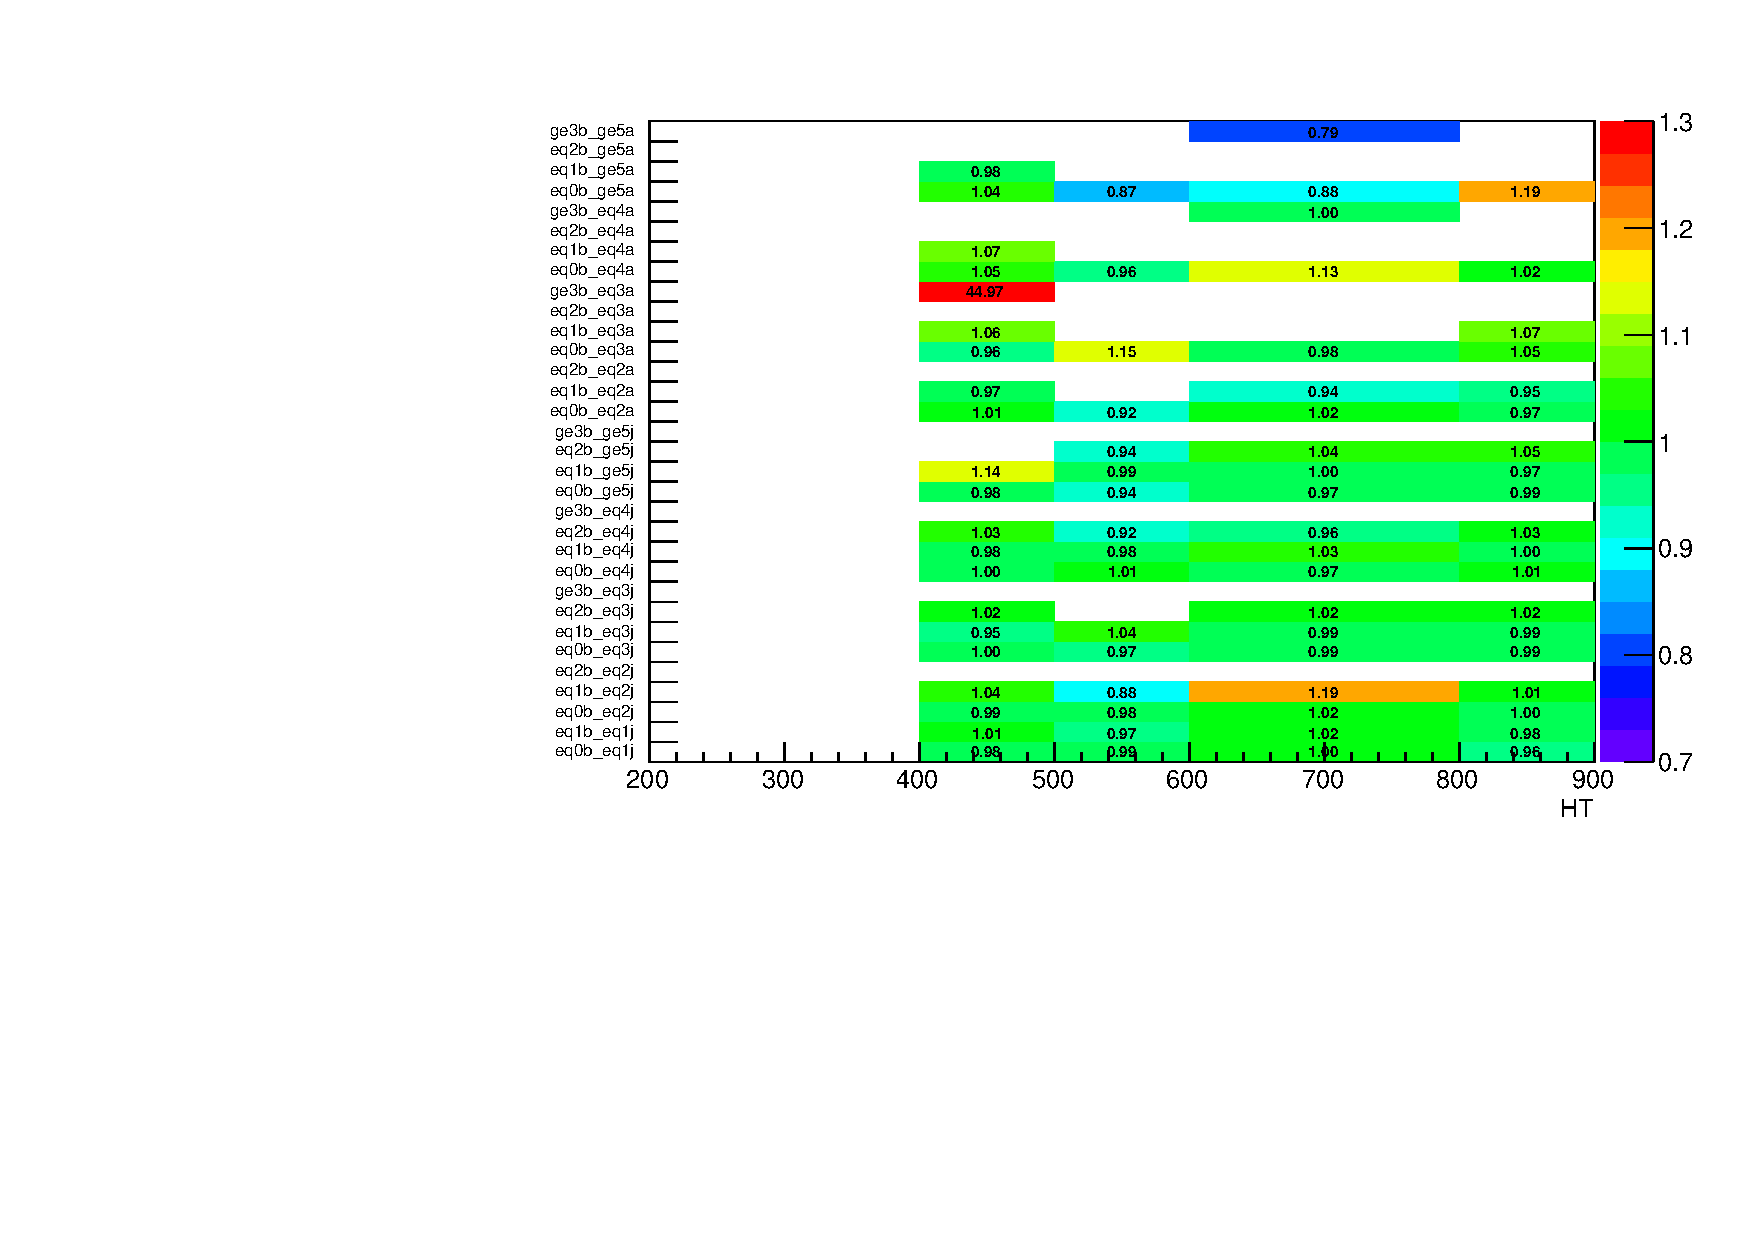
\includegraphics[width=0.5\textwidth]{figs/analysis/systsTf/Zinv/gj/ratiotfh_ht_mht_alljecWeight_Up.pdf}
  } ~~
  \subfloat[JEC down variation]{
    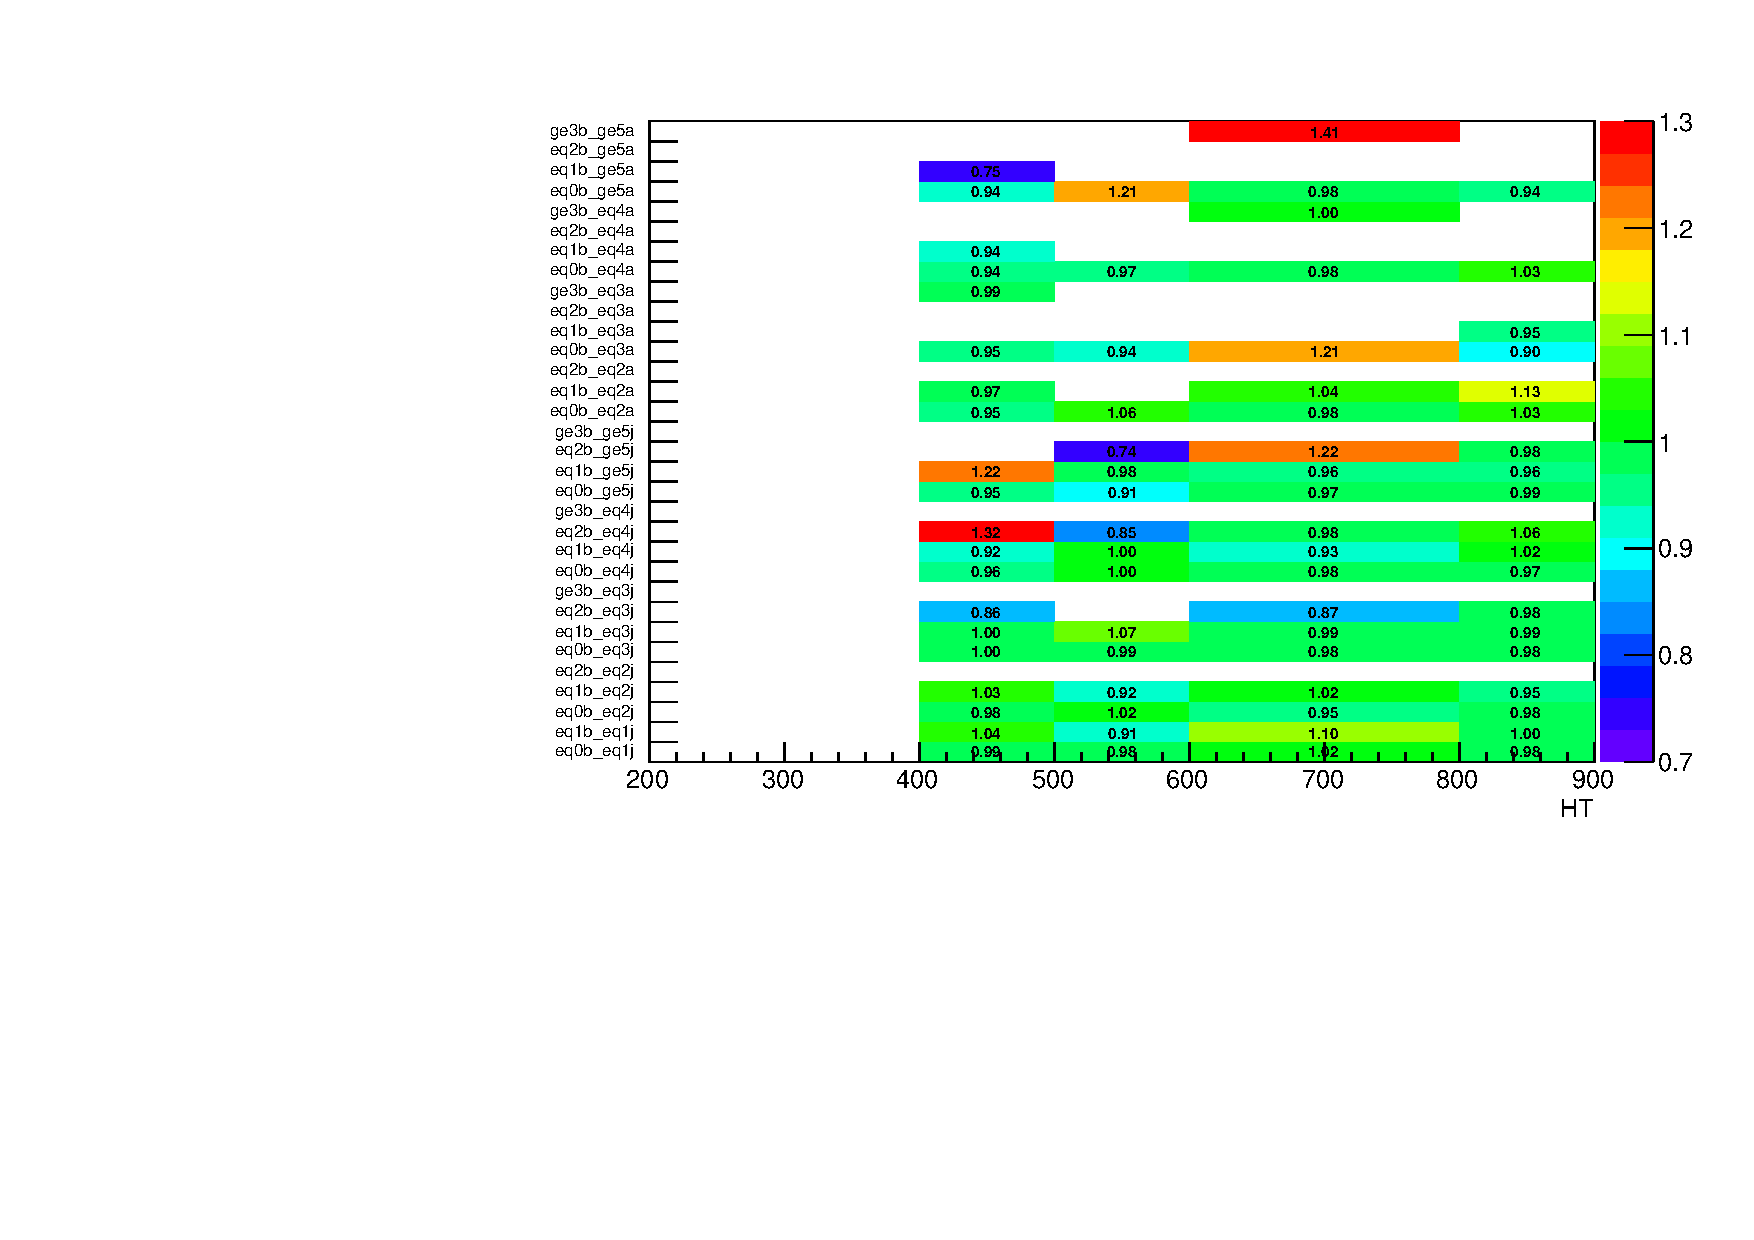
\includegraphics[width=0.5\textwidth]{figs/analysis/systsTf/Zinv/gj/ratiotfh_ht_mht_alljecWeight_Down.pdf}
  }\\

  \caption{\label{fig:tfSyst_jec_gjToZinv} The relative change in the
  $\gj \rightarrow (\znunu)$ transfer
  factors when varying JEC in MC within its uncertainties, as a function of \scalht (GeV) and jet category. 
  Variations corresponding to $+1\sigma$ ($-1\sigma$) are shown in the left (right) figure. The bins are
    labelled as described in App.~\ref{app:plotKey}.
  }
\end{figure}

\begin{figure}[!h]
  \centering
  \subfloat[JEC up variation]{
    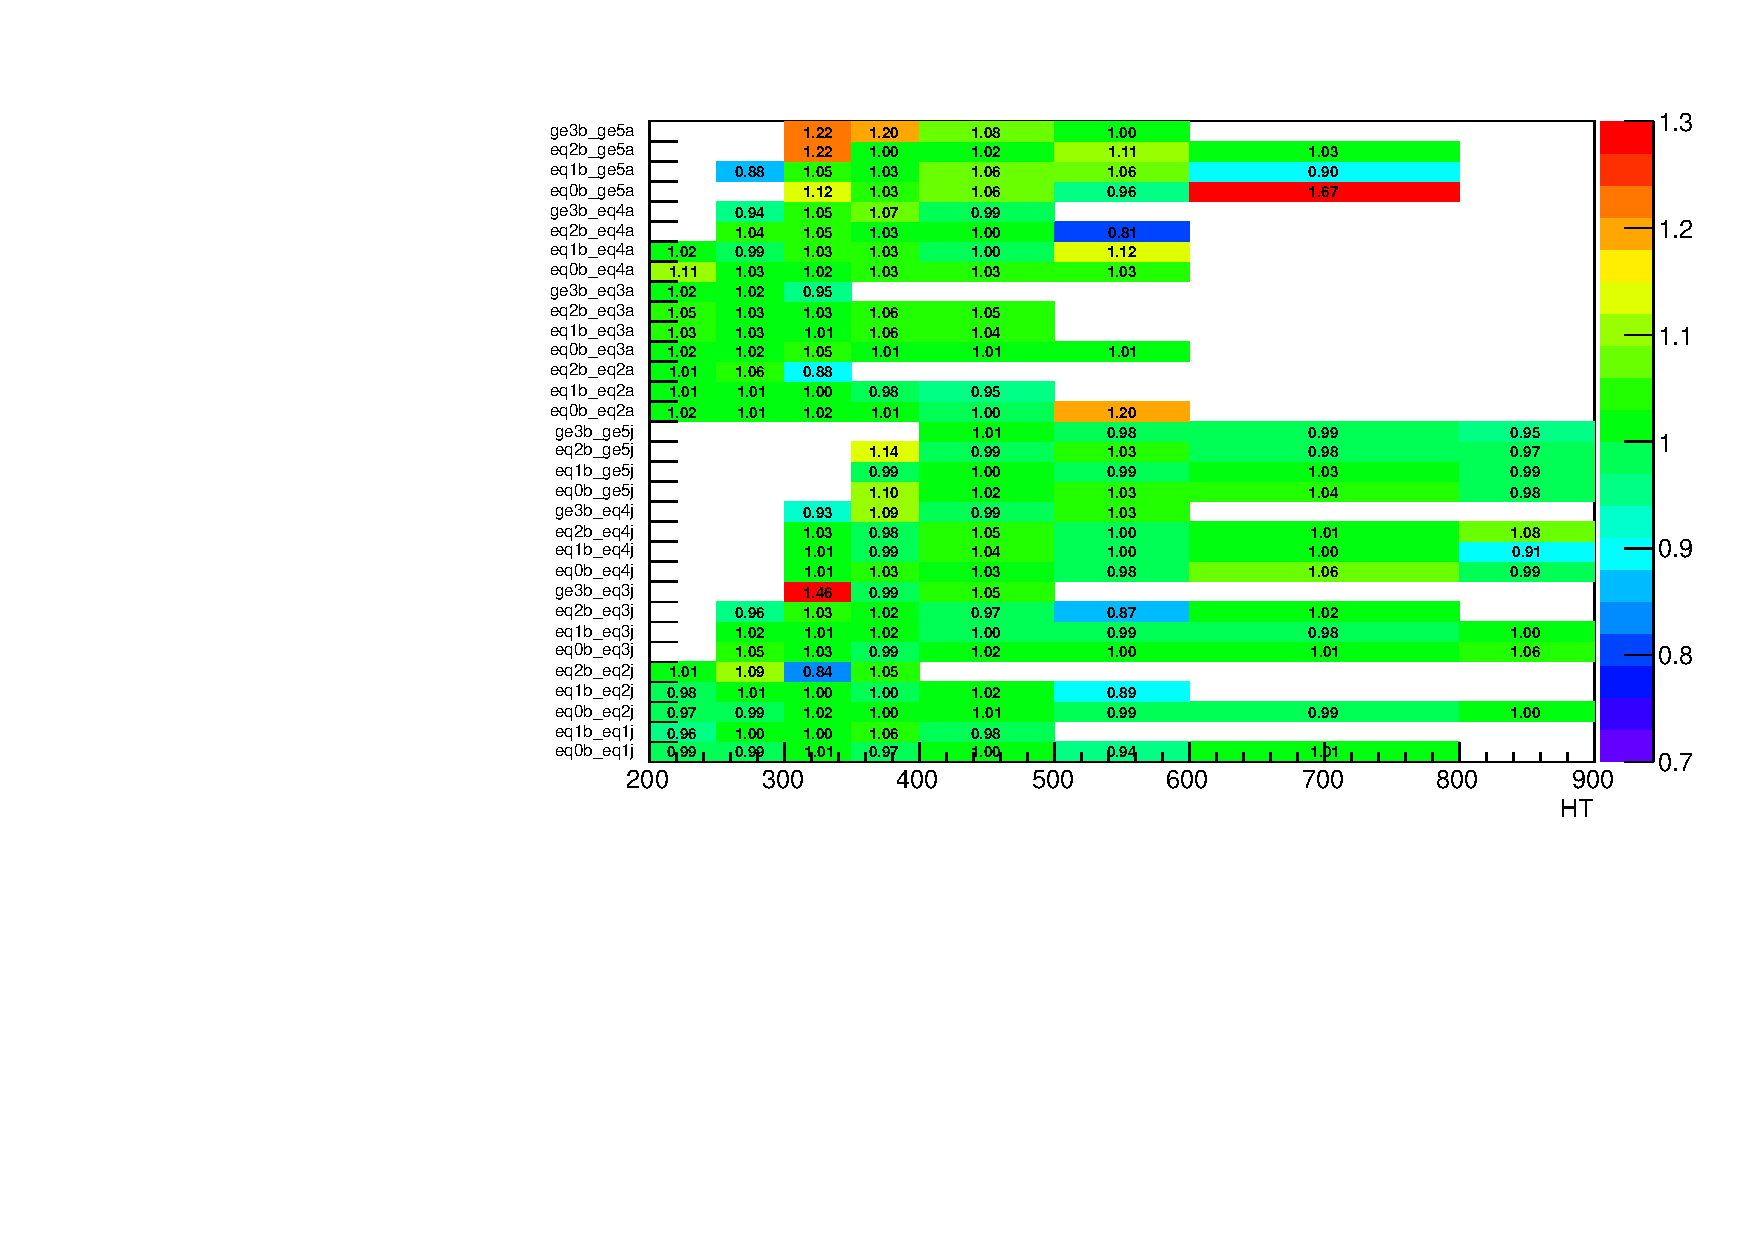
\includegraphics[width=0.5\textwidth]{figs/analysis/systsTf/Ttw/mu/ratiotfh_ht_mht_alljecWeight_Up.pdf}
  } ~~
  \subfloat[JEC down variation]{
    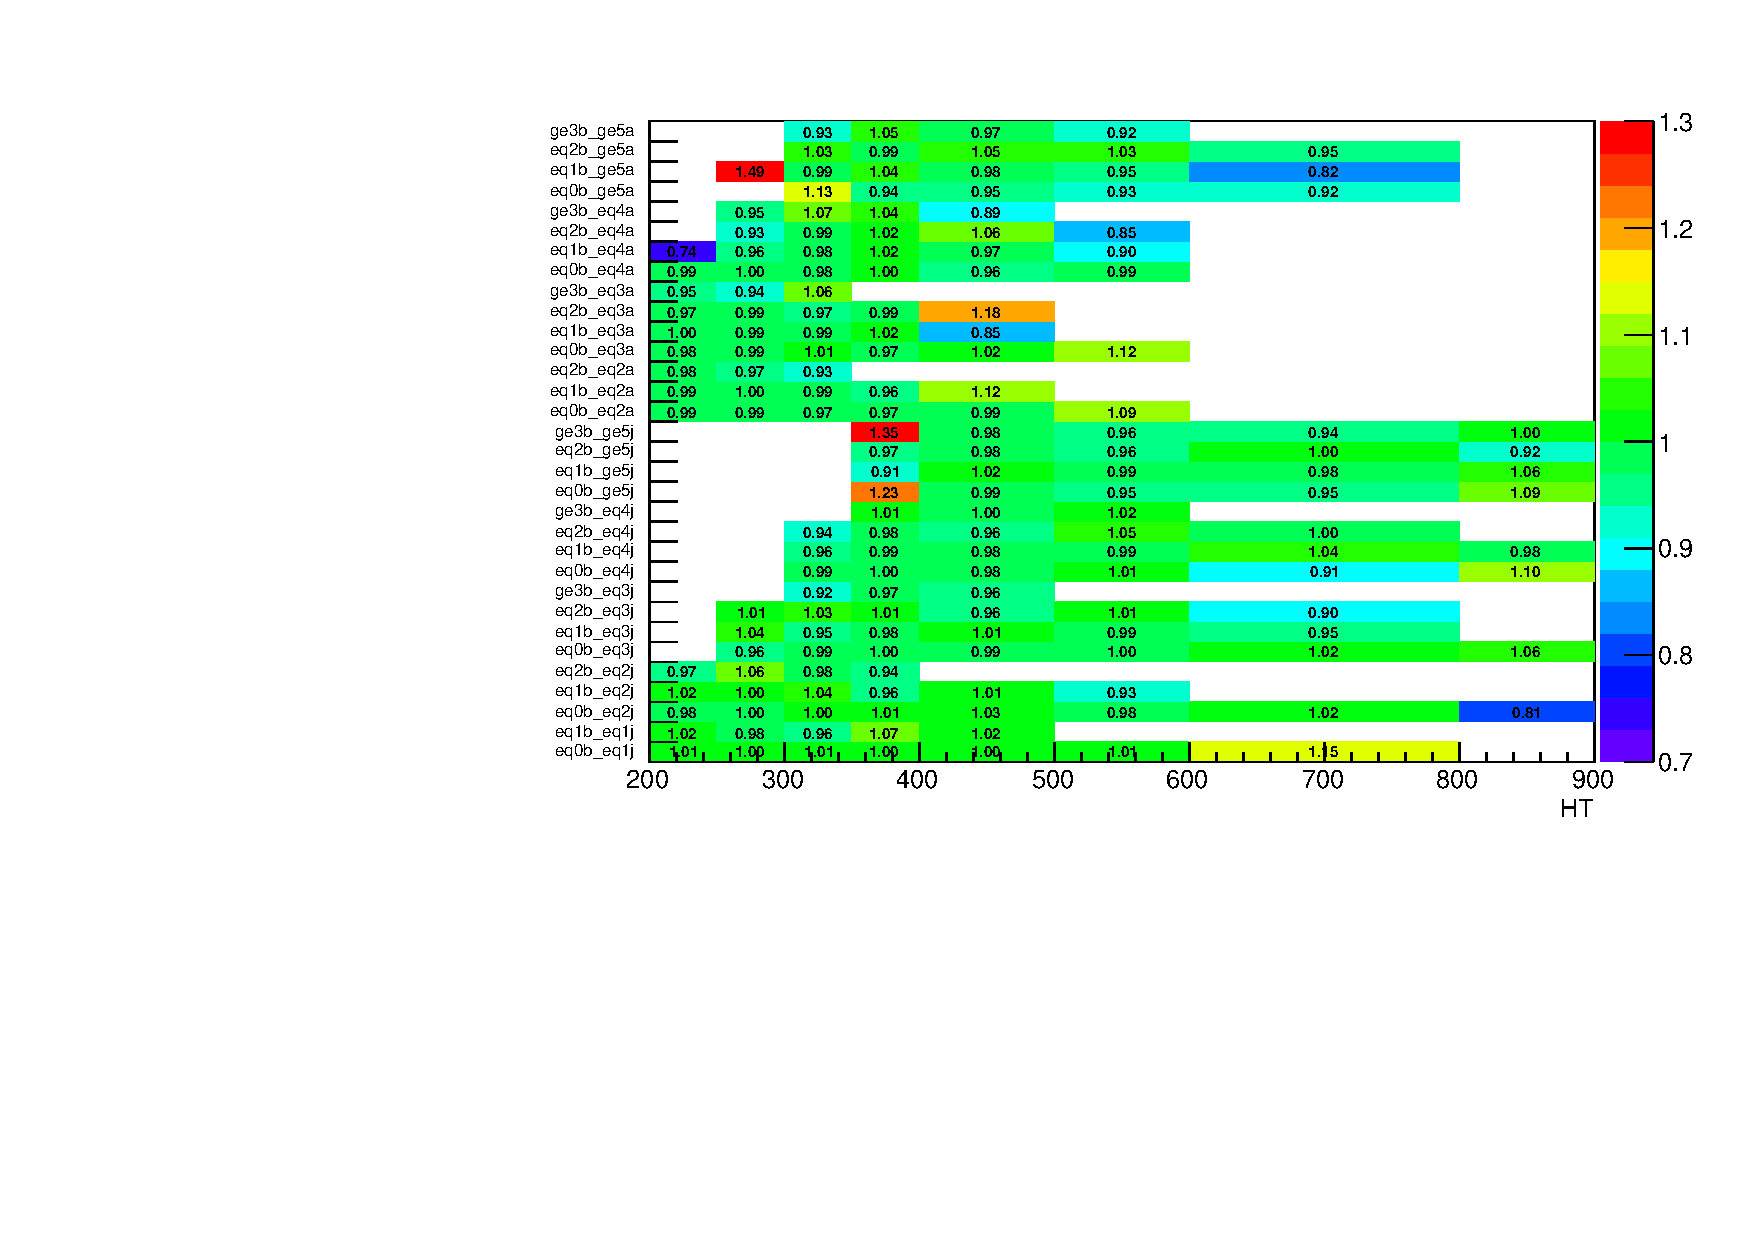
\includegraphics[width=0.5\textwidth]{figs/analysis/systsTf/Ttw/mu/ratiotfh_ht_mht_alljecWeight_Down.pdf}
  }\\

  \caption{\label{fig:tfSyst_jec_muToTtw} The relative change in the
  $\mj \rightarrow \mathrm{\ttbar+W}$ transfer
  factors when varying JEC in MC within its uncertainties, as a function of \scalht (GeV) and jet category. 
  Variations corresponding to $+1\sigma$ ($-1\sigma$) are shown in the left (right) figure. The bins are
    labelled as described in App.~\ref{app:plotKey}.
  }
\end{figure}


\subsubsection*{B-tagging efficiency}
\label{sec:tfSyst_btag}
The scale factors that take account of the b-tagging efficiencies and
misidentification between simulation and data also have associated
uncertainties. Since no extrapolation is performed in the background
prediction across different \nb multiplicities, these uncertainties
are expected to only have a small effect.  The scale factors
associated with the identification of $b$ and c jets are varied together
(since their measurements are correlated), while those associated with
the misidentification of light jets are varied separately. The
relative change in the \TFs is presented as a function of \HT and jet
category in
Fig.~\ref{fig:tfSyst_bsf_muToZinv}-\ref{fig:tfSyst_bsfl_muToTtw}. They
are typically in the range of 1-5\%.

\subsubsection*{Lepton and photon efficiencies}
\label{sec:tfSyst_lepton}

Events from W and \ttbar processes can enter the signal region
when one of the leptons is not identified, by falling out of
acceptance or not being properly reconstructed. There is an uncertainty
associated with these acceptance and reconstruction effects that must
be taken account of.

The uncertainties on the trigger, lepton identification and isolation
efficiencies are varied by $\pm1\sigma$ and their effects on the yield
of W and \ttbar event vetoes is studied.  The procedure is repeated
separately for muons and electrons. There is found to be at most a 2\%
difference in the W and \ttbar yields in the signal region when these
uncertainties are varied. This is propagated as an uncertainty to the
\TFs and taken as correlated across all the signal region bins. 

Along with the considerations of the uncertainties on the simulated
acceptance of leptons, uncertainties in the scale factors can directly
effect yields in the muon control regions. The change in the \TFs with
the upwards and downwards variations of the scale factors of the muons
used to define the single and double muon control regions can be seen
in Figs.~\ref{fig:tfSyst_muon scale
factor_muToZinv}~to~\ref{fig:tfSyst_muon scale factor_muToTtw}. They
are typically in the range 0-3\%.

% The fraction of events with leptons out of acceptance ($f_{sample}$)
% is calculated from generator truth level information for each \MC
% sample. The uncertainties on the trigger, lepton identification and
% isolation efficiencies are encoded in the variable $y$:
% \begin{equation}
%     \label{eq:lostLepTF}
%     y = \frac{\sum_{sample} [ R_{sample} \times f_{sample} \times
%     N^{GEN}_{sample} \times ( 1 - \epsilon_{Loose} ) + ( 1 -
%     f_{sample} ) \times N^{GEN}_{sample} ]}{ \sum_{sample}
%     N^{GEN}_{sample} \times \epsilon_{Tight} \times R_{sample} },
% \end{equation}
% where $R_{sample}$ is the cross section reweighting factor for each
% sample, $N^{GEN}_{sample}$ is the total \MC yield for the category,
% $\epsilon_{Tight}$ and $\epsilon_{Loose}$ are the lepton efficiency
% for the tight and loose working points that are used separately in the
% muon control region and signal region respectively. The variable $y$ is computed for
% each category. For the numerator, the full signal selection is
% applied.  For the denominator, the full selection for the \mj control
% sample is applied.

% Finally, the $\eta$-dependent muon tracking scale factors provided by the muon 
% POG to cover the effect of HIP inefficiencies have been applied and their 
% uncertainties taken into consideration. Their effect on the transfer factors
% is found to be less than 1\%.
%
\subsubsection*{Photon trigger uncertainty}
\label{sec:tfSyst_photonTrigger}

To take account of uncertainties in the photon trigger efficiencies, the
effect of varying them on the \gj \TF is investigated. To make a
conservative estimate of the systematic, the uncertainty on this
correction is taken as the size of the inefficiency. The relative
change in the \gj transfer factor is presented in
Fig.~\ref{fig:tfSyst_photonTrigger_gjToZinv} variation is typically in
the range 0-3\%.

\subsubsection*{Signal trigger uncertainty}
\label{sec:tfSyst_trigger}

The uncertainties on the signal trigger efficiency
measurements must also be taken into account. This is most relevant in the low
\HT and \MHT regions of the analysis, where the triggers are not fully
efficient. As it is possible to measure the efficiency with both muon
and electron reference triggers, a systematic is taken as the
difference in the measurement between the two.  The relative change in
transfer factors is presented in Fig.~\ref{fig:tfSyst_trigger_muToZinv}-\ref{fig:tfSyst_trigger_muToTtw}.
The variation is typically in the range 0-5\%.

\subsubsection*{Top $p_T$ reweighting}
\label{sec:tfSyst_topPt}

To account for the uncertainty on the top \pT reweighting, an 
uncertainty on this correction is taken as the difference of the
correction from unity. The relative change in transfer factors is
presented in Fig.~\ref{fig:tfSyst_topPt_muToZinv}-\ref{fig:tfSyst_topPt_muToTtw}. The
variation is typically in the range 0-15\%.

\subsubsection*{QCD contamination in the \gj control sample}
\label{sec:tfSyst_qcdCont}

Due to the greater prevalence of \QCD multijet background in the \gj
control sample, which is expected to be at the $\sim5\%$ level, an
uncertainty is applied on this contamination. An arbitrarily large
variation of $\pm 100\%$ on the number of simulated \QCD is chosen and
leads to a systematic variation on the \TFs of at most 5\%
in the majority of bins. This value is small enough to remain
subdominant to other uncertainties and is found to be covered in the
data-driven study using the photon control region, described in 
Sec.~\ref{sec:tfSyst_ZGratio}.

\subsubsection*{\PU reweighting}
\label{sec:tfSyst_pu}

There are uncertainties in the minimum bias cross section which is
used to calculate the scale factors for \PU reweighting. This 5\% uncertainty is
propagated and the relative change in the transfer factors under this
variation is small (1-5\%) and shown in each analysis bin in
Fig.~\ref{fig:tfSyst_pu_muToZinv}-\ref{fig:tfSyst_pu_muToTtw}.

%%%%%%%%%%%%%%
\subsection{Uncertainties derived from data driven tests}
\label{sec:closureTests}

To be able to take account of sources of systematic uncertainty that
are not included in the variation of known scale factors, an
additional procedure to derive uncertainties through a data driven
method is defined. This allows assumptions and extrapolations
within the analysis to be covered with an uncertainty that does not
rely on potential limitations in the simulation modelling. To carry
out this data-driven uncertainty estimation process, a suite of
\emph{closure tests} are performed. In each test the number
of events in a given data control (sub-)sample is predicted using
events from another data control (sub-)sample through a
corresponding \TF. The tests are defined in a way that tests a particular assumption made
within the analysis. The agreement between the predicted and observed
yields is expressed as the ratio $(\nobs - \npre)/\npre$ while
considering only the statistical uncertainties on \npre and \nobs,
where \npre is the number of predicted events in the (sub-)sample and
\nobs the number observed.  This allows one to define a level of
\emph{closure}, which encapsulates the statistical significance of a
deviation in the ratio from zero. The significance with which
this closure deviates from zero can then be used to approximate the
systematic uncertainty associated to the assumption the procedure is
testing within the analysis.

These closure tests are performed separately for each \njet category,
as a function of \HT. The systematic uncertainty in each \HT bin
is derived by summing in quadrature the ratio $(\nobs - \npre)/\npre$
with its statistical error, after merging the \njet categories into
their symmetric and asymmetric topologies. Pairs of \HT bins are merged
when the $\mu\mu$+jets sample is used, in order to increase the
statistical power of the sample.  Since the uncertainties derived with
this approach are statistical in nature, these systematics are
considered uncorrelated in each \HT bin and event topology category. 

\subsubsection*{Extrapolation in \alphat and \bdphi}
\label{sec:tfSyst_alphaT}

There is no \bdphi cut made in any of the control regions and no
\alphat cut in the muon control regions. As this is the case, it is
implicitly assumed that the simulation correctly models the
distribution of both of these variables when the \TFs are constructed.
To provide an estimate of the systematic uncertainty related to this
assumption, dedicated closure tests are carried out.  
% In both cases, it is checked that
% events with genuine \met found in the core of the variable
% distribution below some threshold value can be used to predict the
% events in the tail (above the same threshold value).  This is
% important to verify the approach of using \mj and \mmj samples without
% an \alphat requirement to make background predictions in the signal
% region. 
The tests are carried out in the \mj control region, using data yields
with an \alphat or \bdphi requirement to predict the data yield of
events with this requirement inverted. Explicitly for the \alphat
closure tests, the number of
predicted events, $N^{\alphat>x}_{pred}$, is: 
\begin{equation}
N^{\alphat>x}_{pred} =
\frac{N^{\alphat>x}_{MC}}{N^{\alphat<x}_{MC}}\times N^{\alphat<x}_{obs} 
\end{equation}
where $N^{\alphat<x}_{obs}$ is the number of events that fail the
\alphat requirement $x$, $N^{\alphat<x}_{MC}$ is the number of simulated
events that fail the requirement and $N^{\alphat>x}_{MC}$ is the
number of events that pass the requirement. The closure is then
defined as:
\begin{equation}
(N^{\alphat>x}_{obs}-N^{\alphat>x}_{pred})/N^{\alphat>x}_{pred},
\end{equation}
where $N^{\alphat>x}_{obs}$ is the number of observed events that pass
the \alphat requirement.

The result of these tests are shown in Fig.~\ref{fig:closureAlphaT} as
a function of \scalht and \njet.  The grey band is the systematic
uncertainty propagated through the analysis, taken as un-correlated
per each \scalht bin and jet topology (symmetric/asymmetric). The
systematic derived from these tests is in the range $4-32\%$.

The \bdphi and \alphat closure tests are testing the same kind of
extrapolation, in a topological \met based variable. As this is the
case the contribution to the systematic error is taken from only the
\alphat closure tests for bins with $\scalht<800\gev$ and from the
\bdphi tests for bins with $\scalht>800\gev$.

\begin{figure}[h!]
  \begin{center}
    \subfloat[]{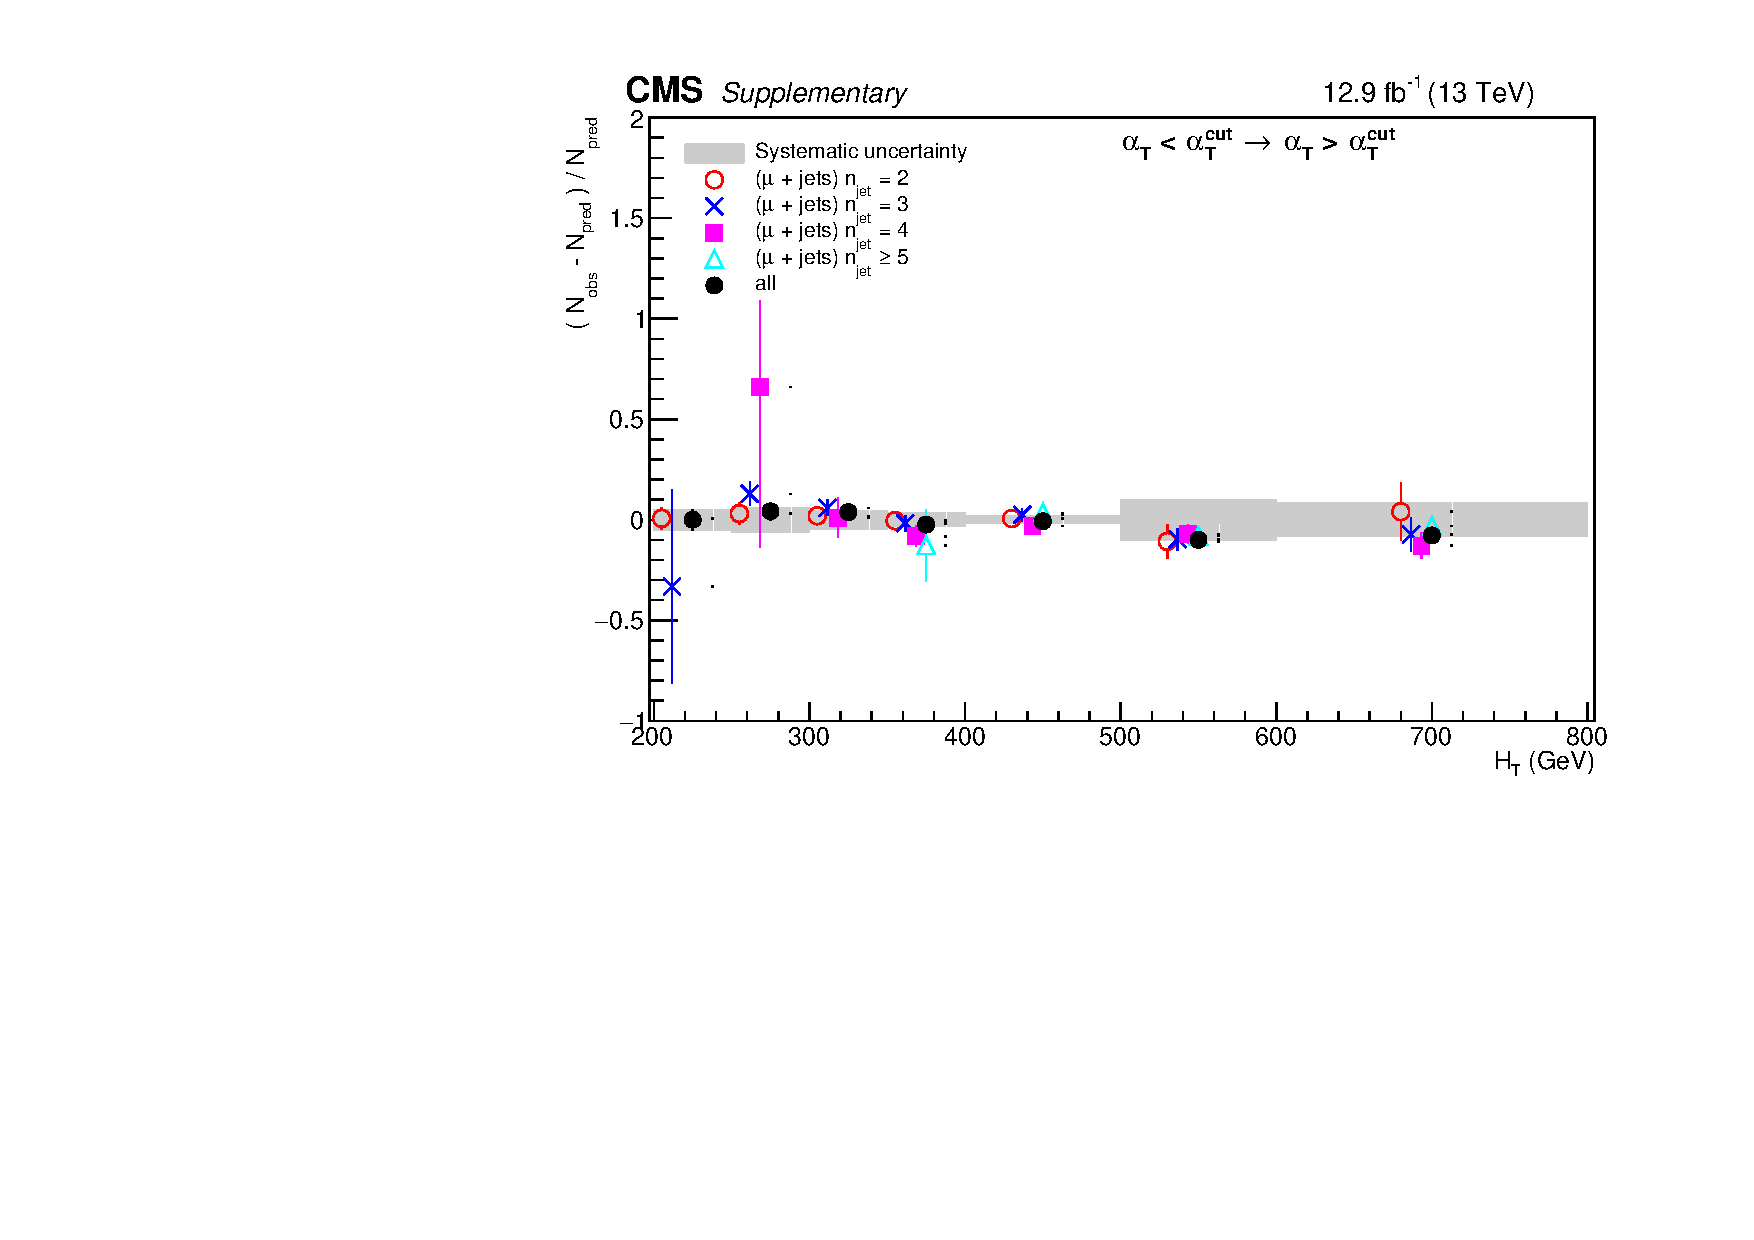
\includegraphics[width=0.5\textwidth]{figs/analysis/closureTests/alphaT_sym__noFit.pdf}}
    ~~
    \subfloat[]{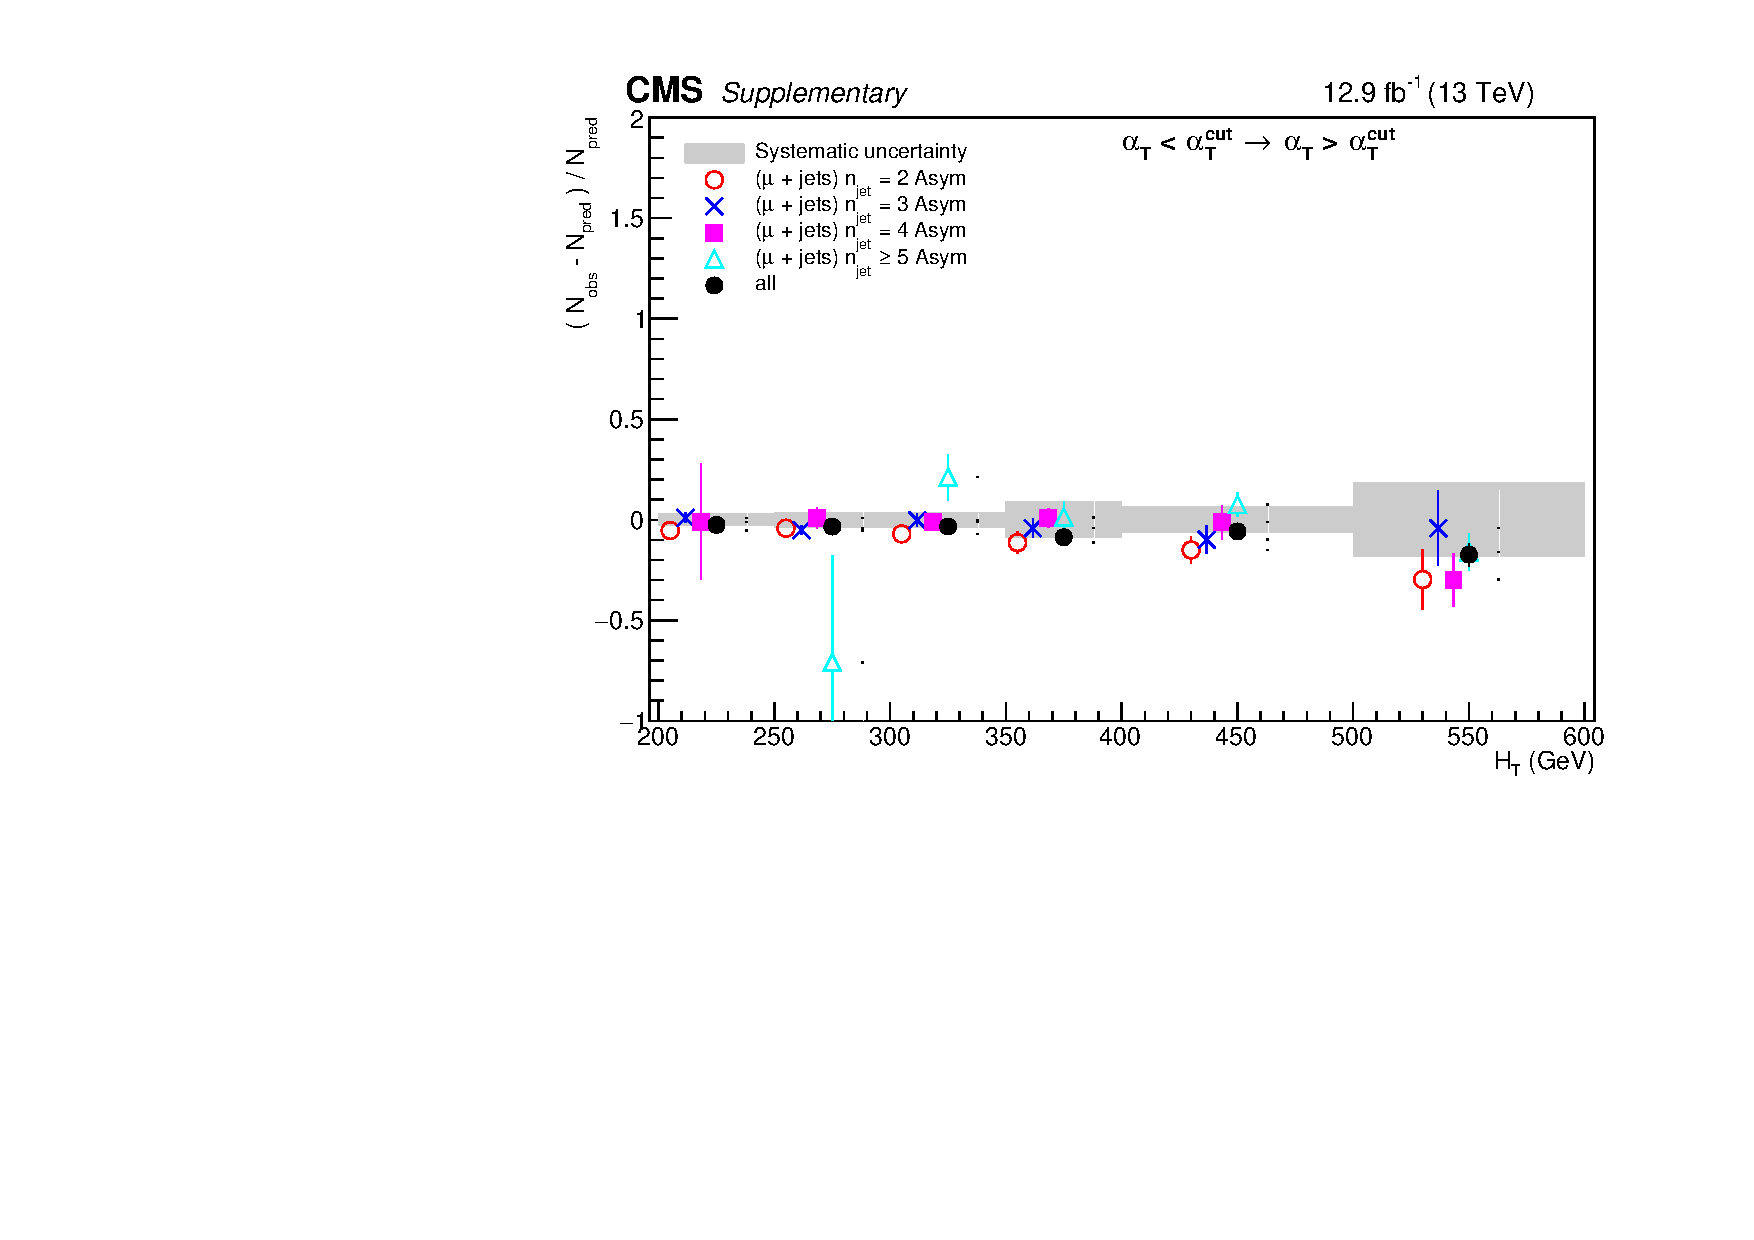
\includegraphics[width=0.5\textwidth]{figs/analysis/closureTests/alphaT_asym__noFit.pdf}}\\
    \subfloat[]{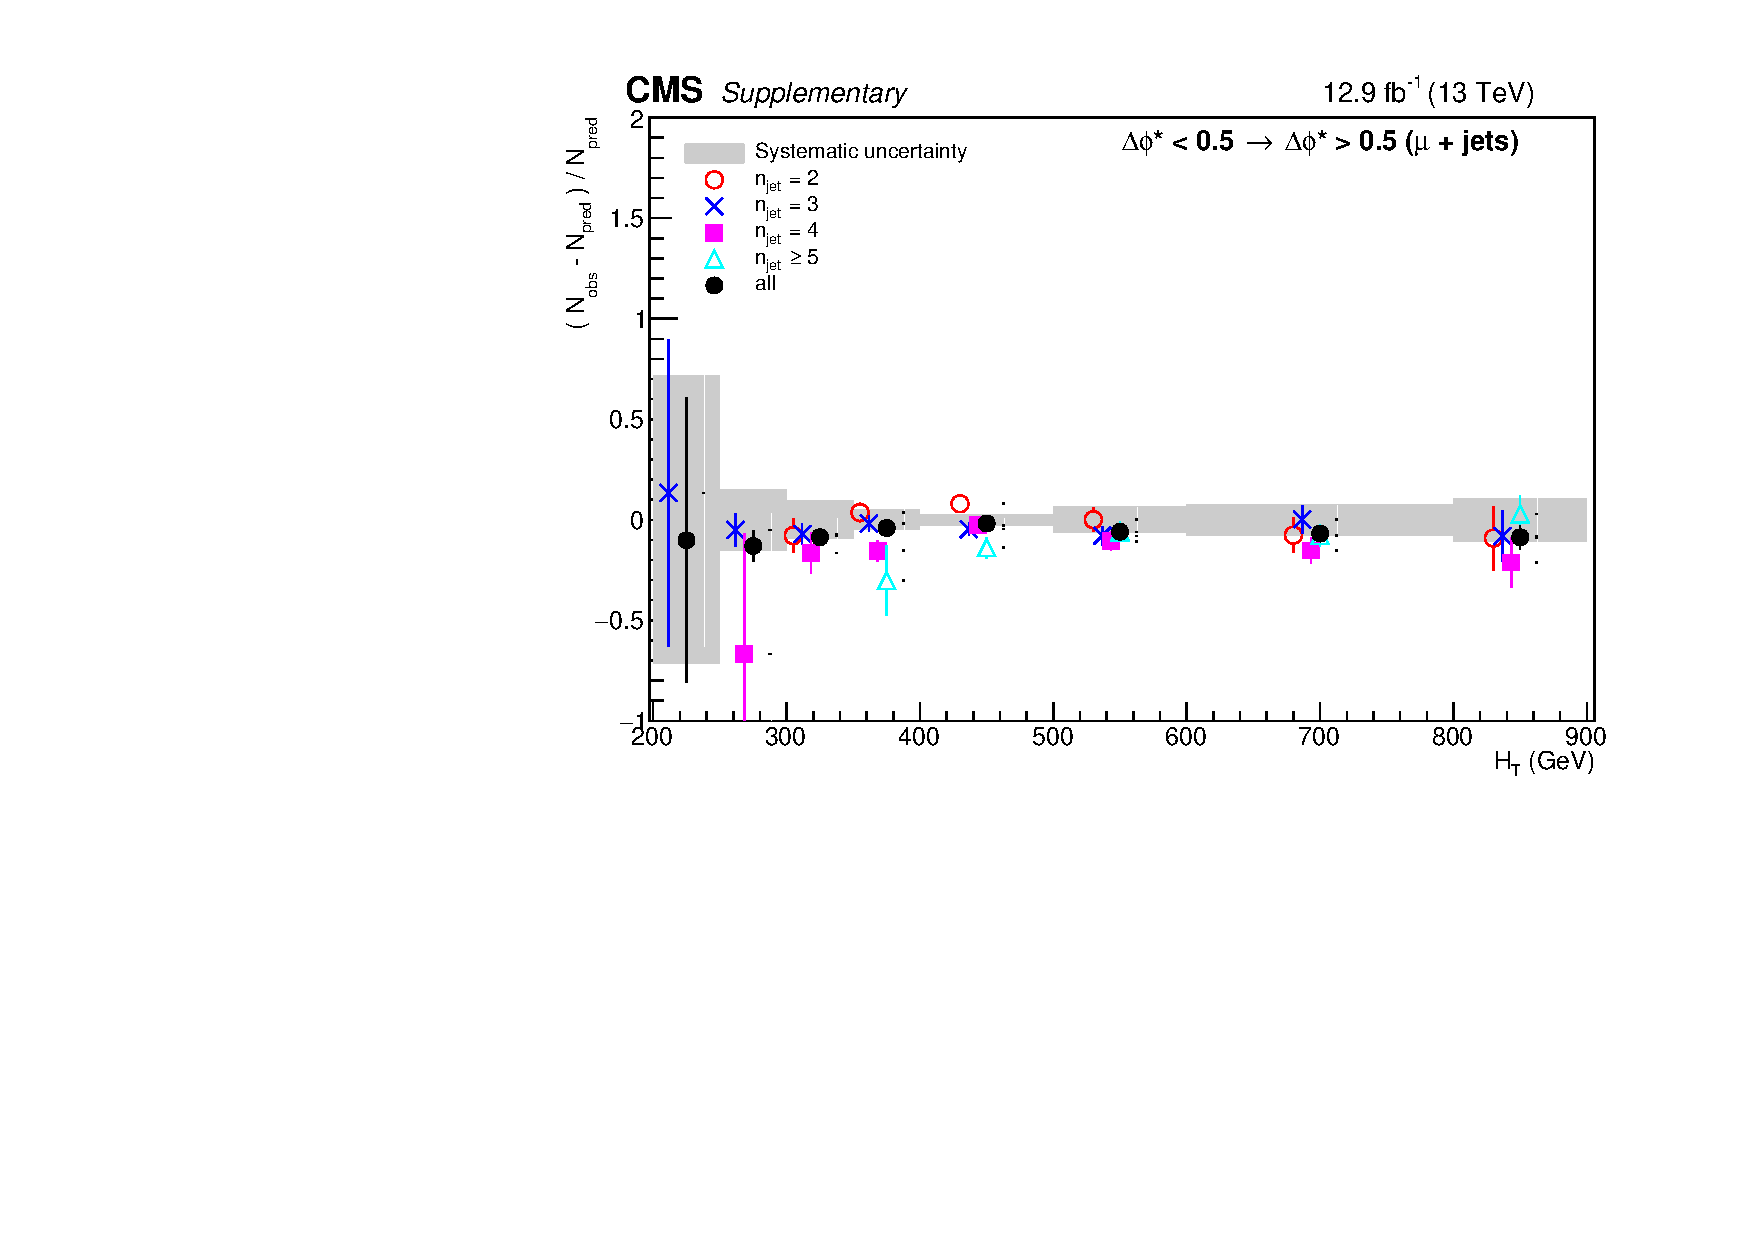
\includegraphics[width=0.5\textwidth]{figs/analysis/closureTests/bDPhi_sym__noFit.pdf}}
    ~~
    \subfloat[]{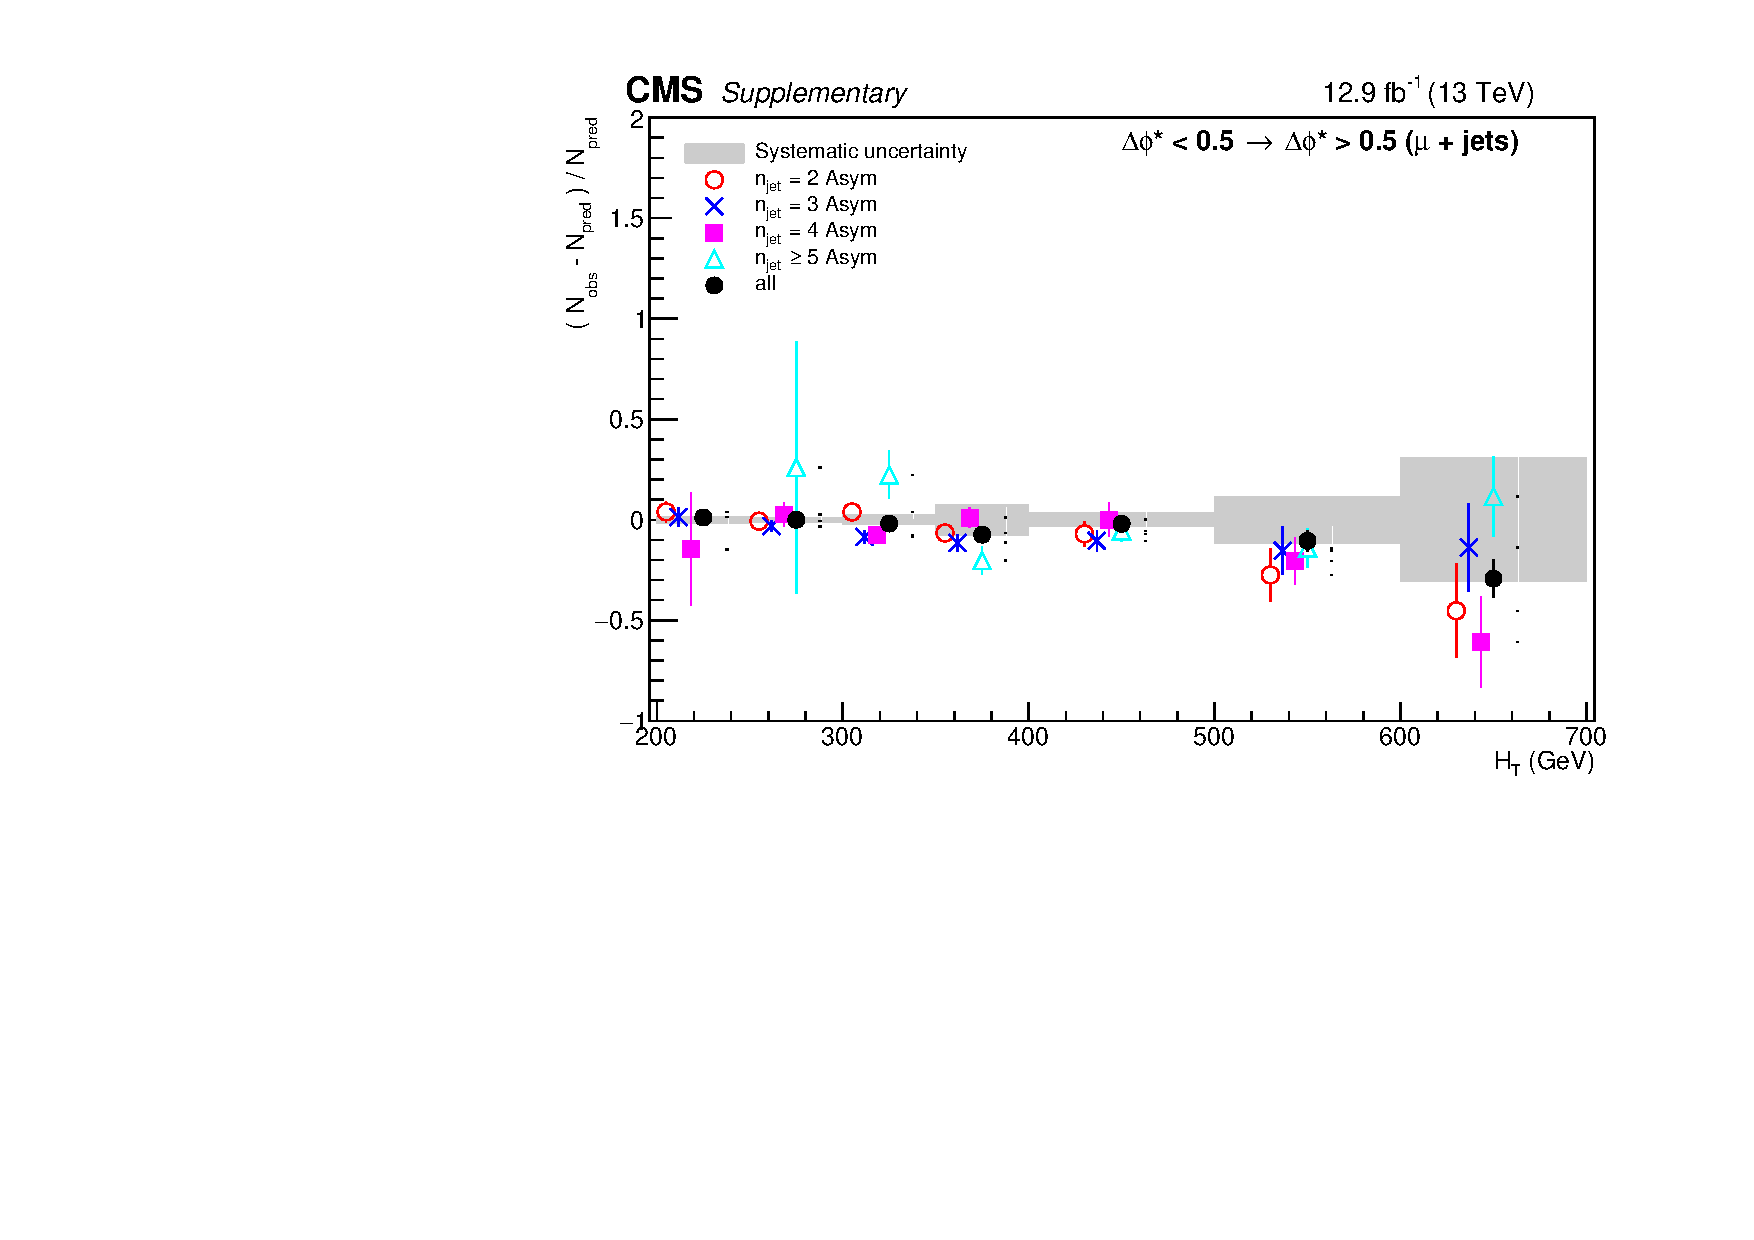
\includegraphics[width=0.5\textwidth]{figs/analysis/closureTests/bDPhi_asym__noFit.pdf}} 

    \caption{Data-driven tests probing the \alphat (top row) and \bdphi (bottom row) extrapolation for each
      \njet category (open symbols) overlaid on top of the systematic
      uncertainty estimates used for each of the seven \scalht bins (shaded bands). 
      The symmetric (asymmetric) jet topologies are shown in the left (right) plot. 
    }
    \label{fig:closureAlphaT}
  \end{center} 
\end{figure}

\subsubsection*{Modelling of the W/Z ratio}
\label{sec:tfSyst_WZratio}
To validate the use of \wmj and \ttbar dominated \mj events to predict
the \znunu background, tests are performed in data using single-muon
and double-muon control regions.  The events in the \mj control region are
used to predict events in the \mmj control region, using transfer
factors from simulation.  These tests target the modelling of the W/Z
ratio in simulation and also indirectly test muon acceptance effects,
which are expected to be sub-dominant and whose uncertainties are
already addressed elsewhere.

The result are shown in Fig.~\ref{fig:closureMuToMuMu} as a function
of \scalht and \njet.  The grey band is the systematic uncertainty
propagated through the analysis, taken as un-correlated per each
\scalht bin and jet topology (symmetric/asymmetric). The systematic
derived from these tests is in the range $3-20\%$.

\begin{figure}[h!]
  \begin{center}
    \subfloat[]{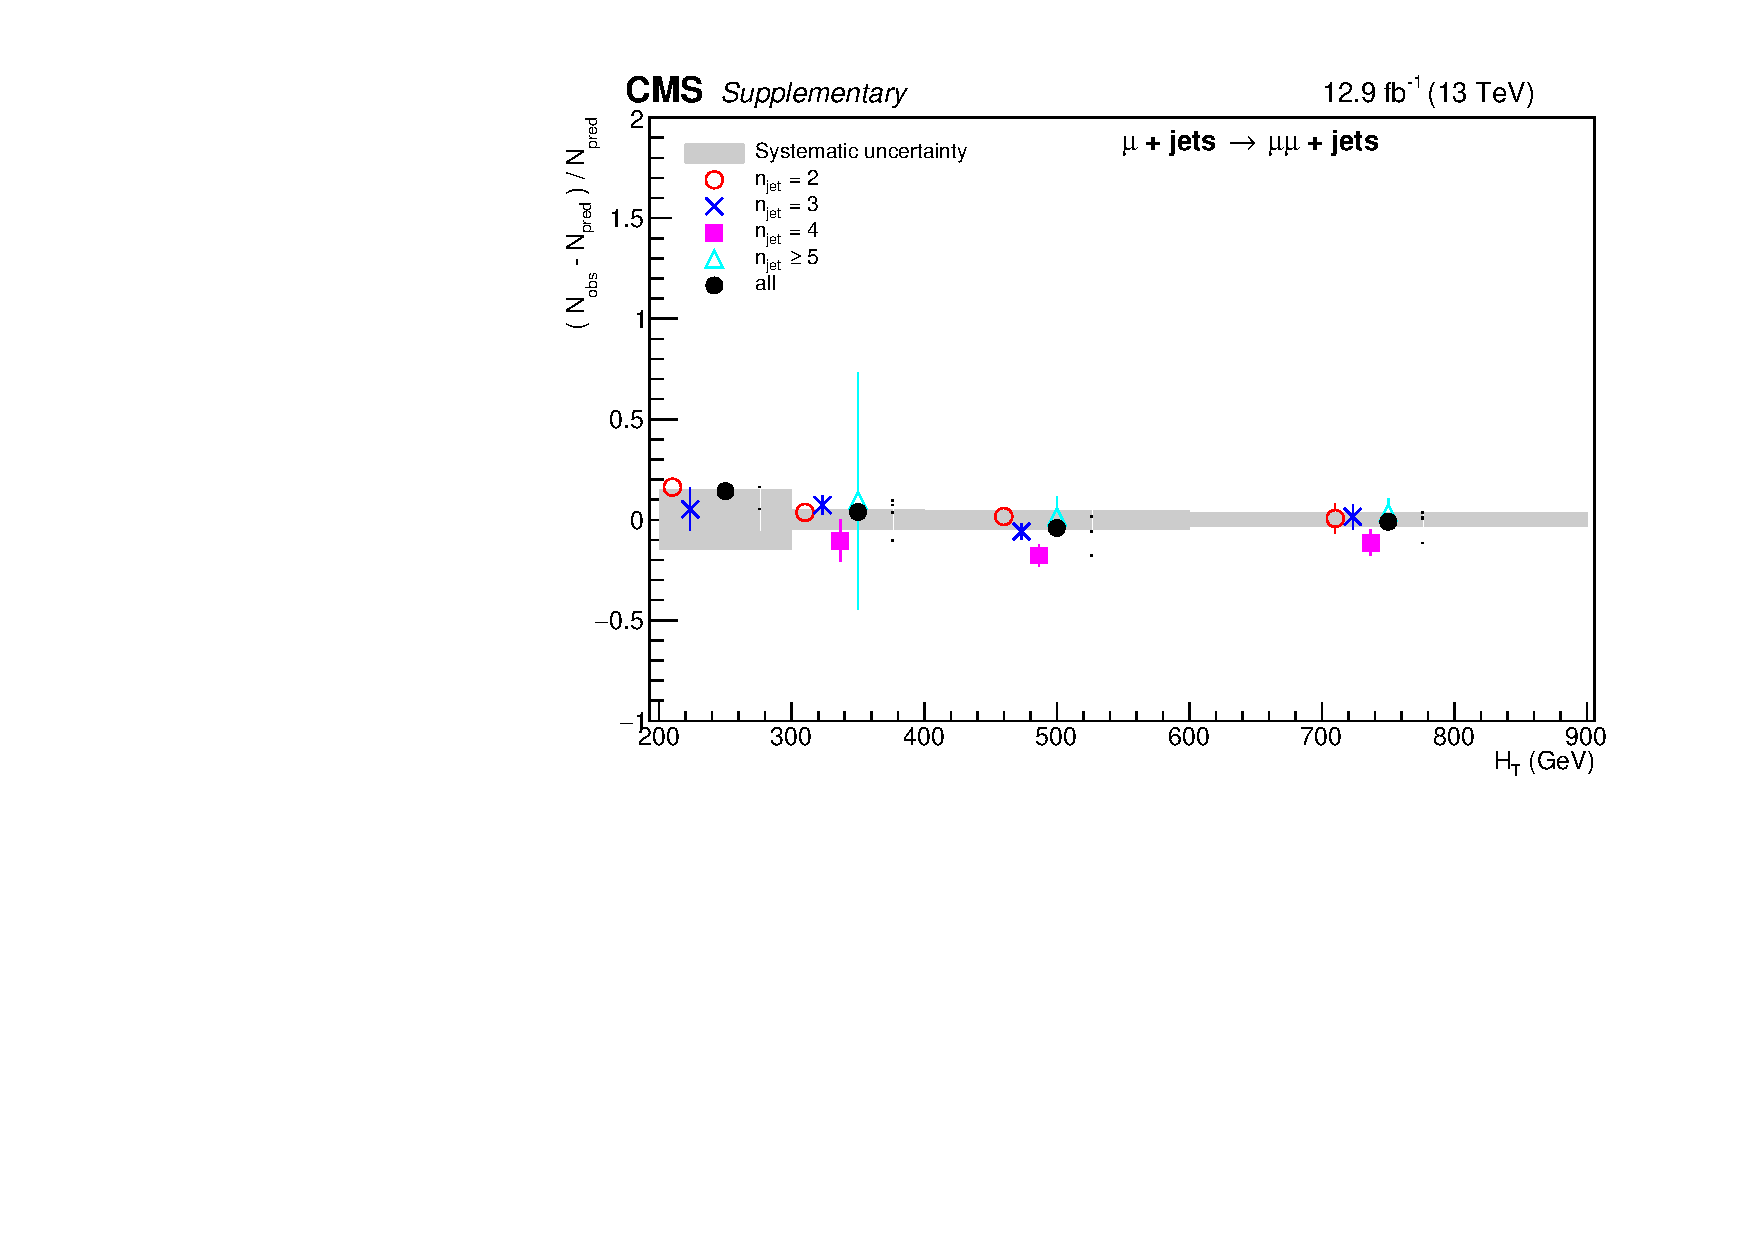
\includegraphics[width=0.5\textwidth]{figs/analysis/closureTests/mu_mumu_sym_half_noFit.pdf}}
    ~~
    \subfloat[]{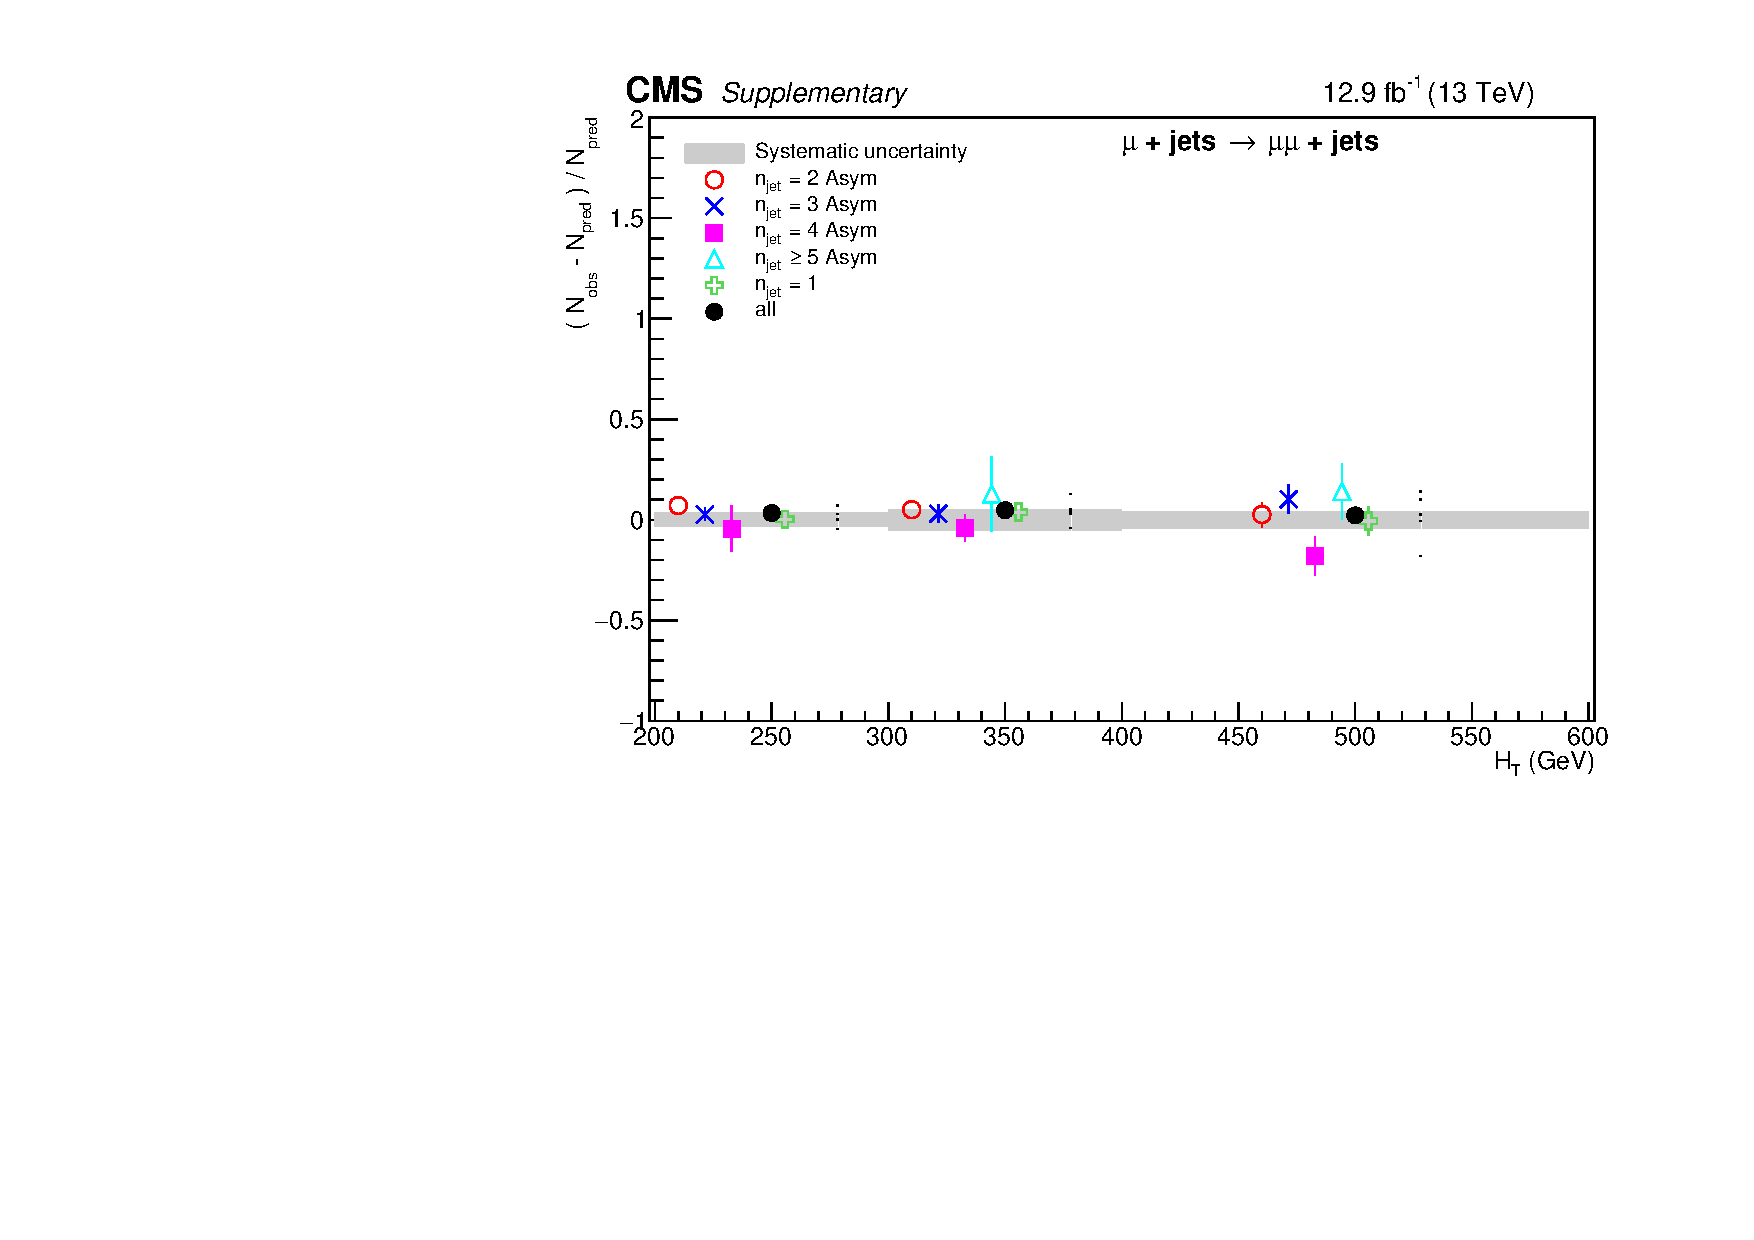
\includegraphics[width=0.5\textwidth]{figs/analysis/closureTests/mu_mumu_asym_half_noFit.pdf}} 
    \caption{Data-driven tests probing the use of the \mj control sample
      to predict the \znunu background for each
      \njet category (open symbols) overlaid on top of the systematic
      uncertainty estimates used for each of the seven \scalht bins (shaded bands).  
      The symmetric (asymmetric) jet topologies are shown in the left (right) plot. 
    }
    \label{fig:closureMuToMuMu}
  \end{center} 
\end{figure}

\subsubsection*{Modelling of the W/Z acceptance due to polarisation effects}
\label{sec:tfSyst_Wpol}

As the kinematics of $W^+$ and $W^-$ decays are subtly different, a
data-driven test is introduced to check the modelling of this effect
in simulation. In this study, carried out with events in the \mj
control region, yields $\mu^{+}$ events are used to predict the yields
of $\mu^{-}$ events.  The production mechanism of W bosons from
$pp$-collisions means high $p_T$ W-bosons are predominantly left
handed \cite{WPol}.  For high $p_T$ bosons, this implies that $W^+$
decays to the left handed neutrino along its direction of motion while
the lepton is pointing backward.  The opposite behaviour is expected
for the $W^-$. The lepton is therefore more boosted (and the neutrino
less boosted) in $W^+$ decays than $W^-$ decays.  This leads to a
larger number of $W^+$ decays in the single lepton control regions
(which relies on the lepton $p_T$ for acceptance) than in the signal
region (which relies on the neutrino $p_T$ for acceptance).

The results are shown in Fig.~\ref{fig:closureMuPToMuM} as a function
of \scalht and \njet.  The grey band is the systematic uncertainty
propagated through the analysis, taken as un-correlated per each
\scalht bin and jet topology (symmetric/asymmetric). The systematic
derived from these tests is in the range $3-12\%$.

\begin{figure}[h!]
  \begin{center}
    \subfloat[]{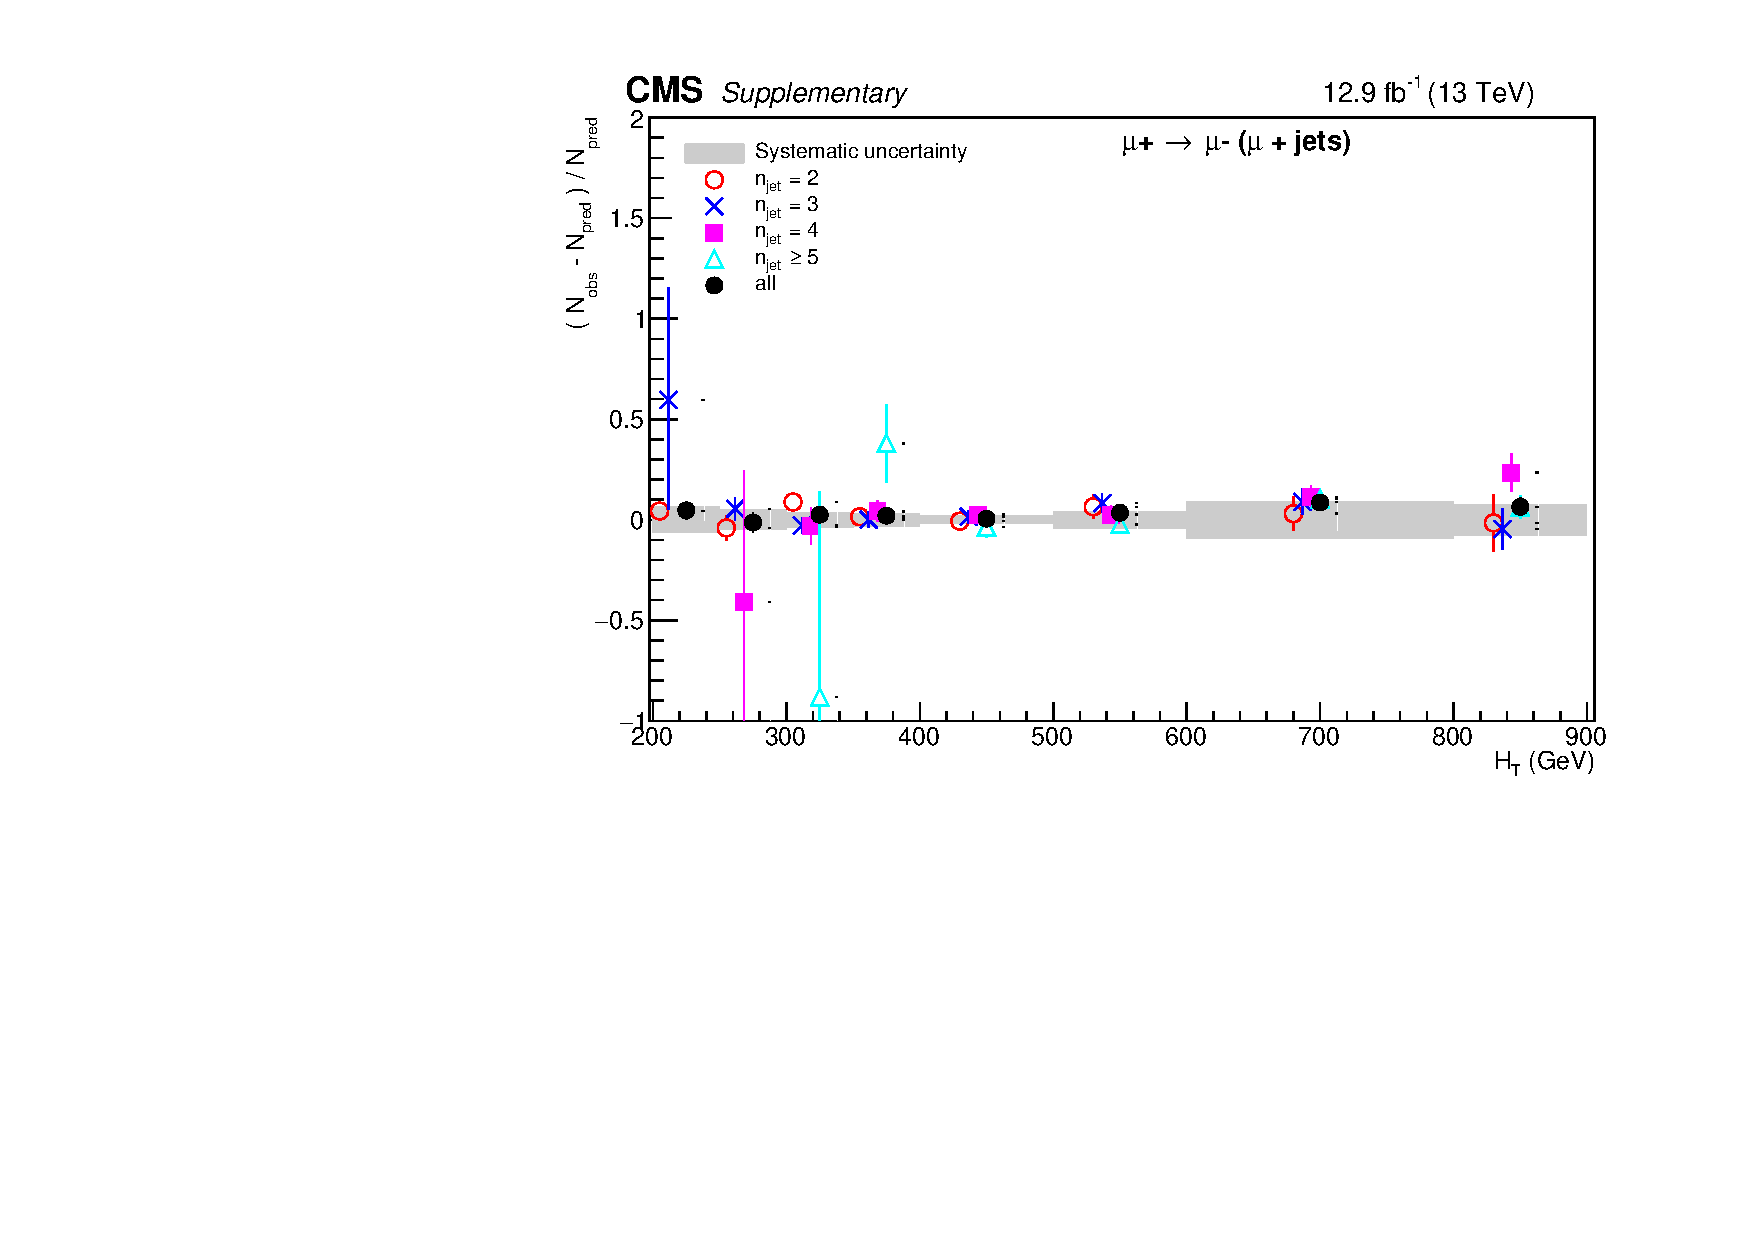
\includegraphics[width=0.5\textwidth]{figs/analysis/closureTests/muplus_muminus_sym__noFit.pdf}}
    ~~
    \subfloat[]{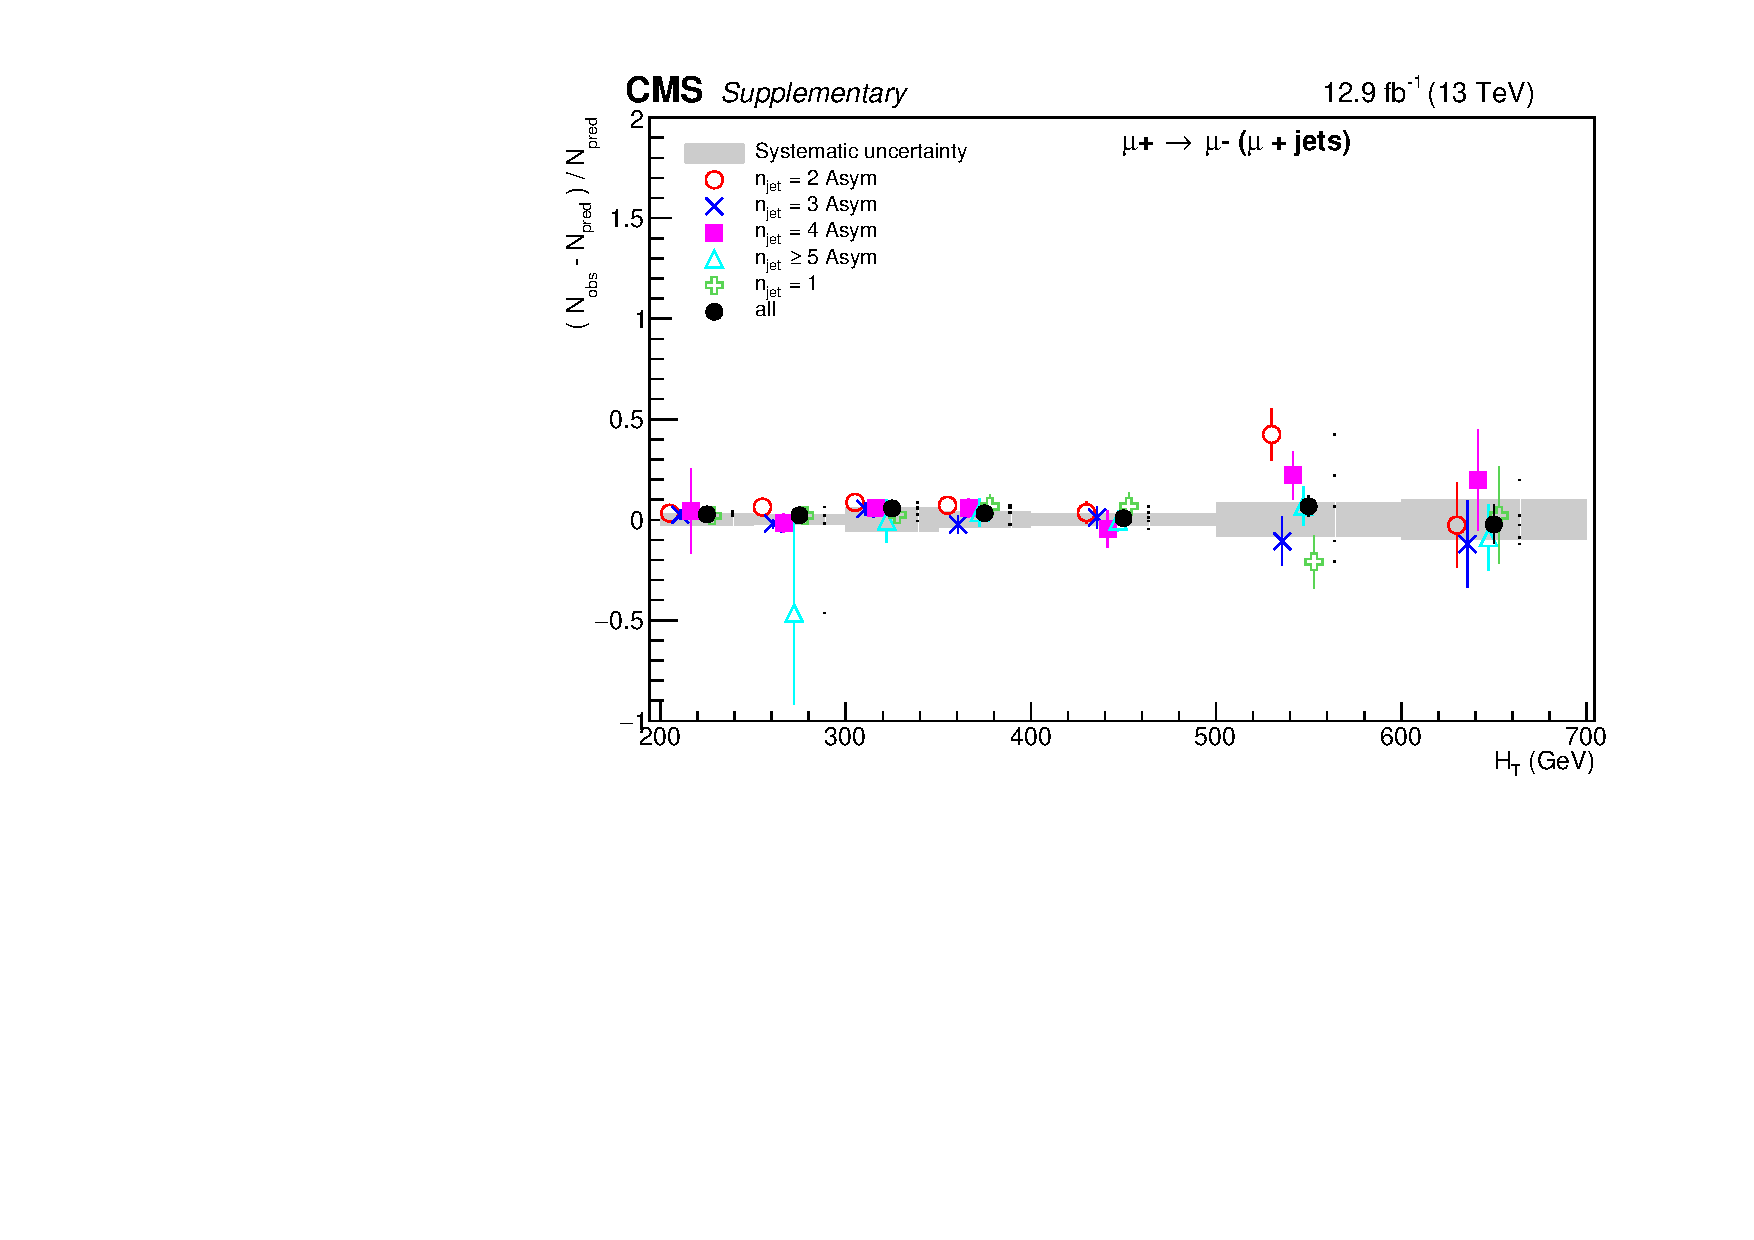
\includegraphics[width=0.5\textwidth]{figs/analysis/closureTests/muplus_muminus_asym__noFit.pdf}} 
    \caption{Data-driven tests probing the W polarisation effects. 
      These are shown for each
      \njet category (open symbols) overlaid on top of the systematic
      uncertainty estimates used for each of the seven \scalht bins
      (shaded bands). 
      The symmetric (asymmetric) jet topologies are shown in the left (right) plot.       
    }
    \label{fig:closureMuPToMuM}
  \end{center} 
\end{figure}

\subsubsection*{Modelling of the Z/$\gamma$ ratio}
\label{sec:tfSyst_ZGratio}
To validate the use of \gj events to predict the \znunu background,
tests are performed in data using the photon and double-muon control
regions. The events in the \gj control are used to predict events in
the \mmj control regions, again using transfer factors from simulation.
These tests target the modelling of the Z/$\gamma$ ratio in simulation
and also indirectly test muon/photon acceptance effects, which,
however, are expected to be sub-dominant and whose uncertainties are
already addressed elsewhere. 

The result are shown in Fig.~\ref{fig:closurePhoToMuMu} as a function
of \scalht and \njet.  The grey band is the systematic uncertainty
propagated through the analysis, taken as un-correlated per each
\scalht bin and jet topology (symmetric/asymmetric). The systematic
derived from these tests is in the range $7-15\%$.

\begin{figure}[h!]
  \begin{center}
    \subfloat[]{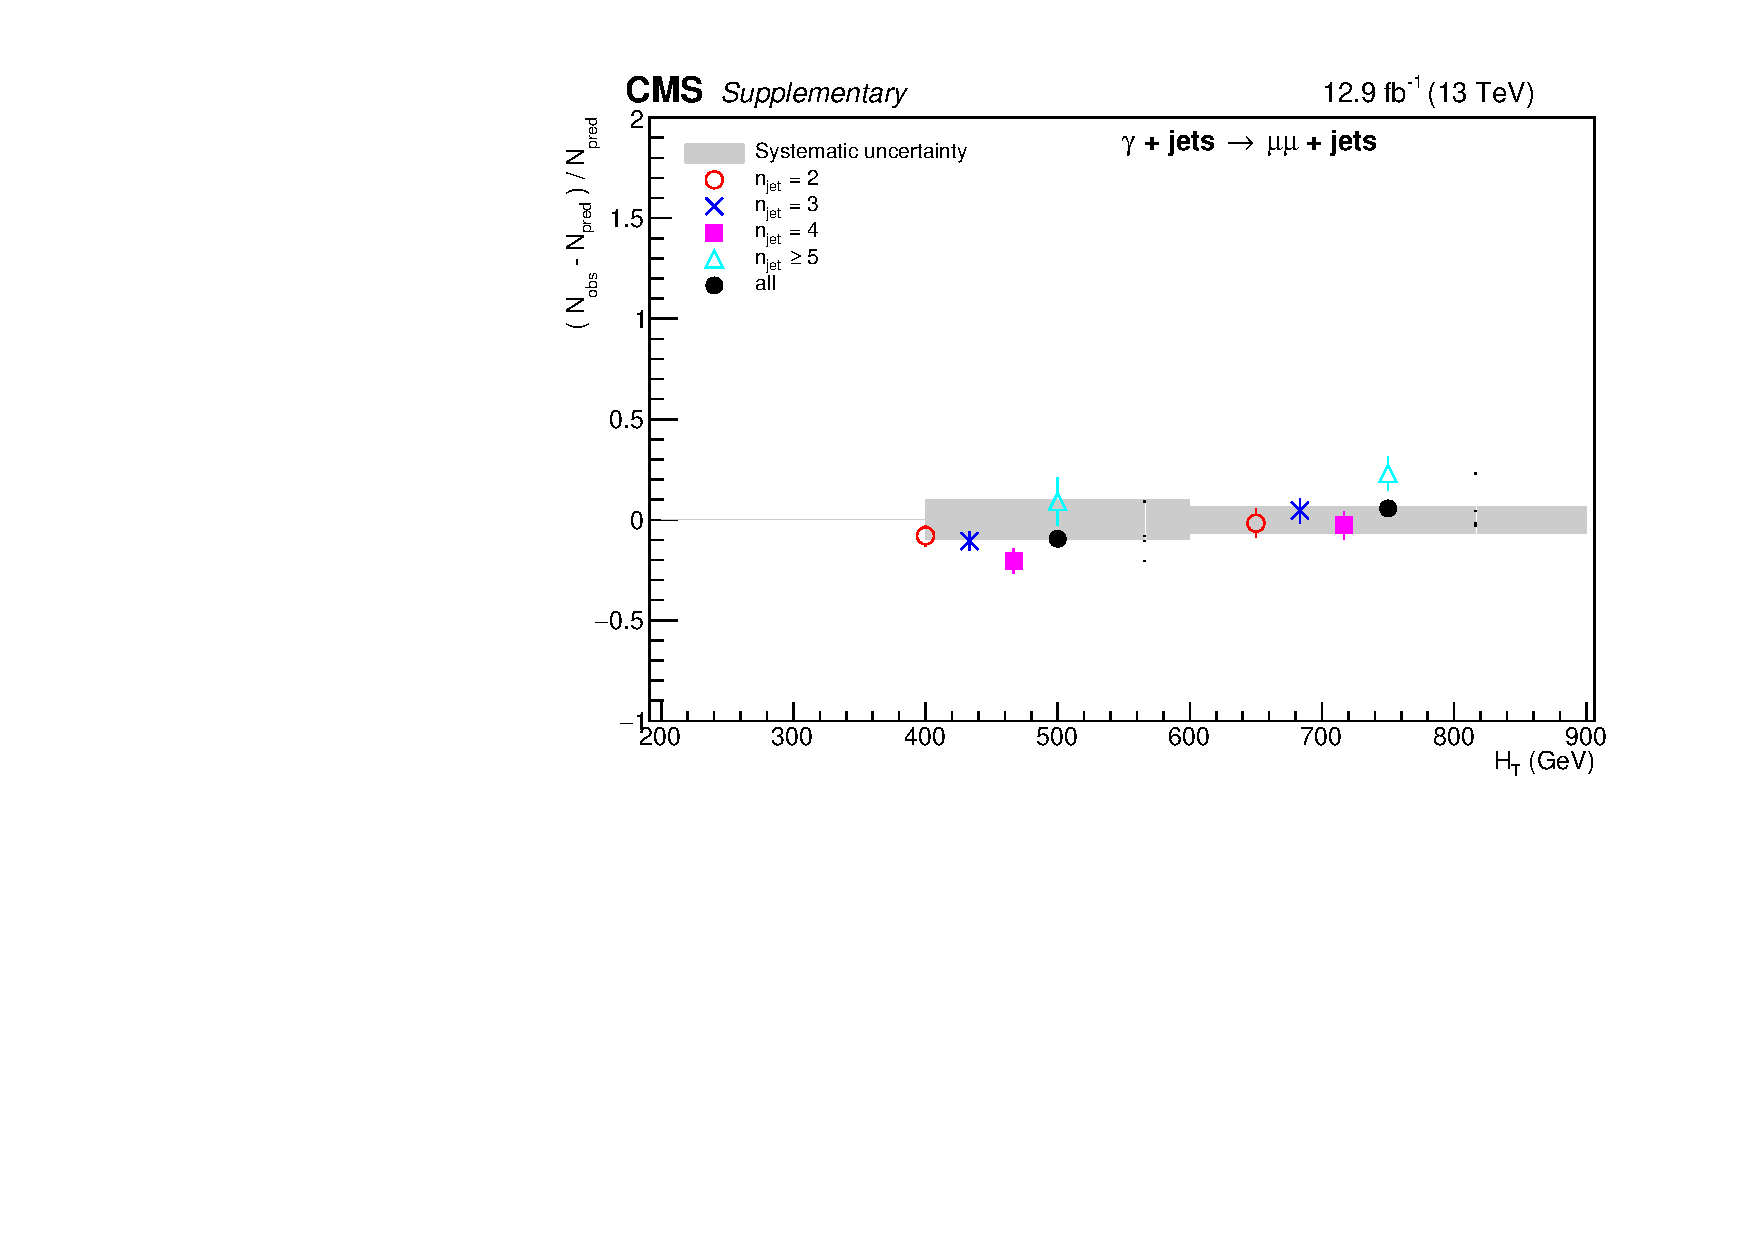
\includegraphics[width=0.5\textwidth]{figs/analysis/closureTests/phot_mumu_sym_half_noFit.pdf}}
    ~~
    \subfloat[]{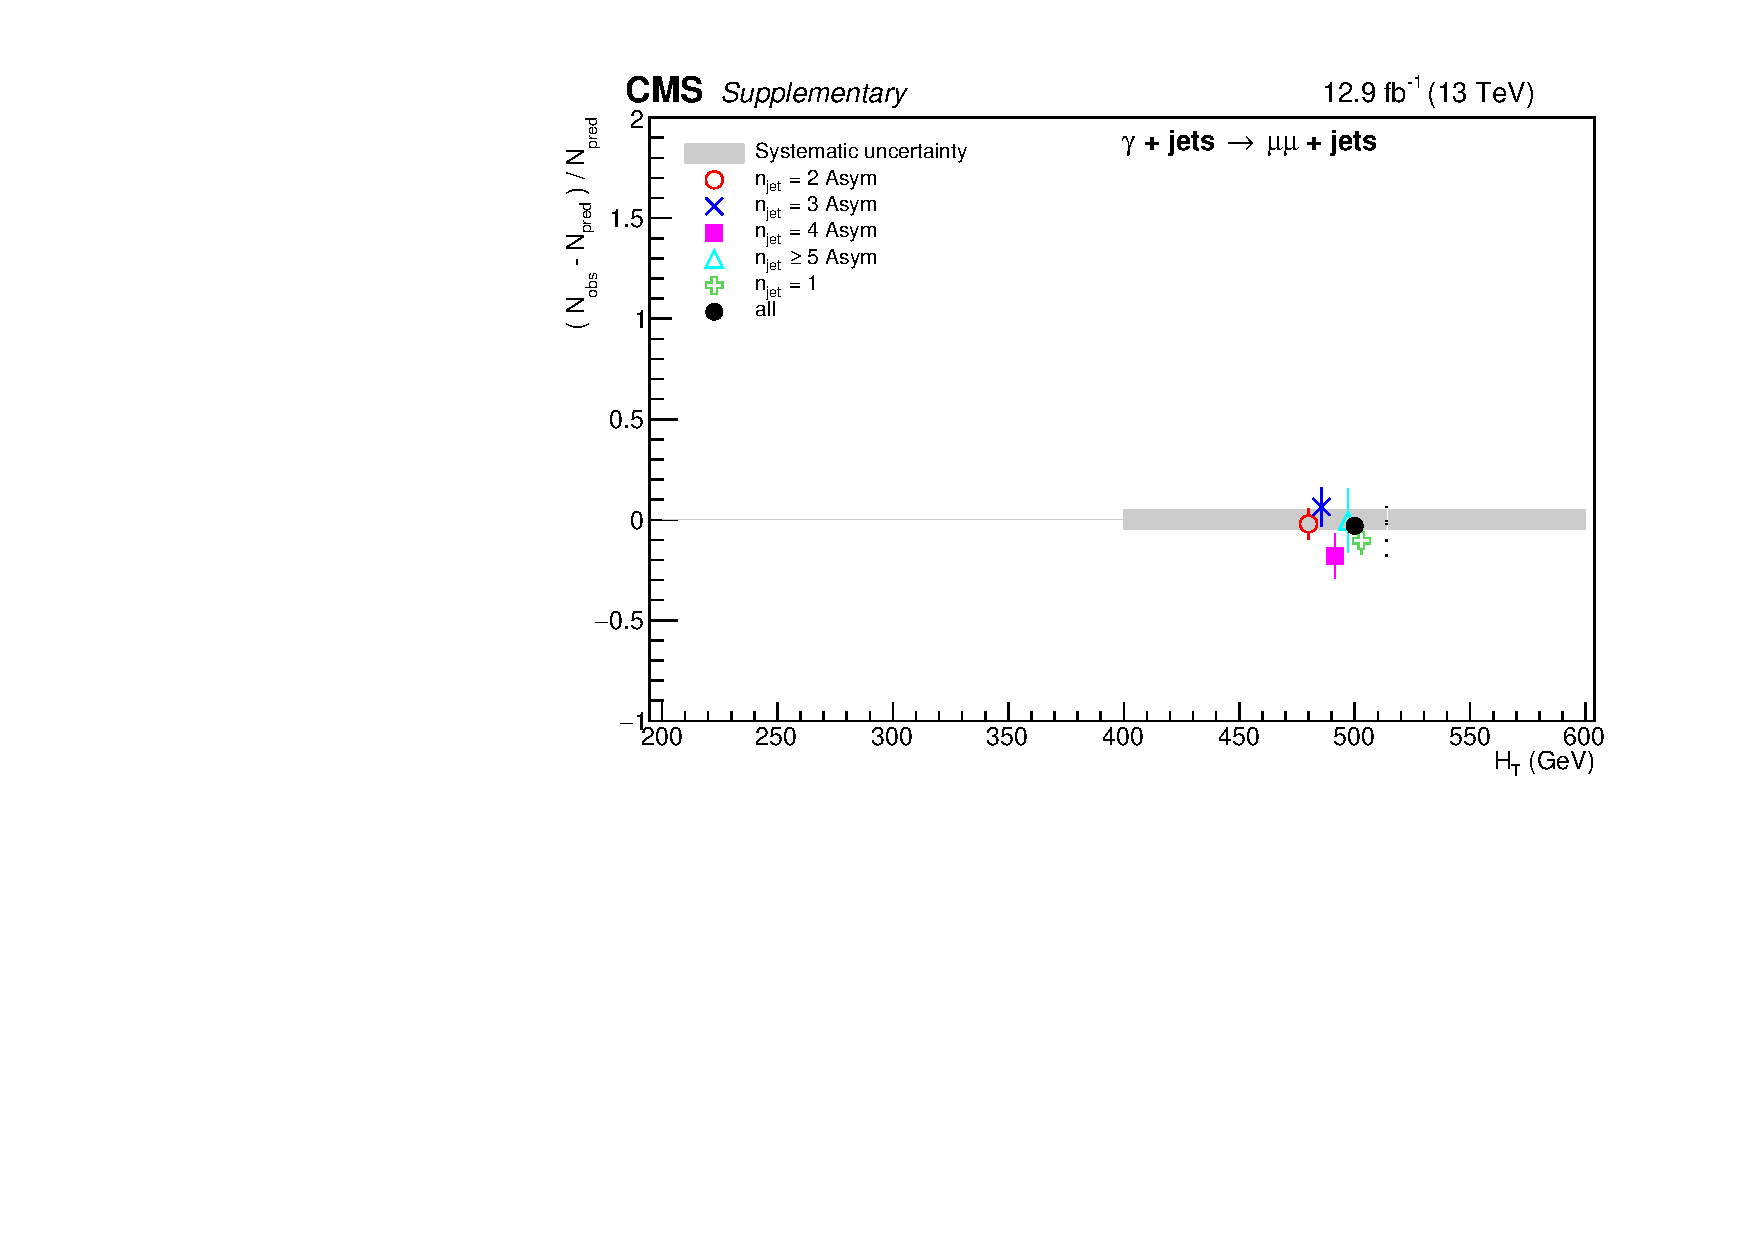
\includegraphics[width=0.5\textwidth]{figs/analysis/closureTests/phot_mumu_asym_half_noFit.pdf}} 
    \caption{Data-driven tests probing the Z/$\gamma$ ratio for each
      \njet category (open symbols) overlaid on top of the systematic
      uncertainty estimates used for each of the seven \scalht bins
      (shaded bands). 
      The symmetric (asymmetric) jet topologies are shown in the left (right) plot.      
    }
    \label{fig:closurePhoToMuMu}
  \end{center} 
\end{figure}

\subsubsection*{Modelling of the W/\ttbar admixture}
\label{sec:tfSyst_WttAd}

The $0$ b-tag $\rightarrow1$ b-tag data-driven tests in the \mj
control region probe the sensitivity of the \TFs to the
relative admixture of events from the \wj and \ttbar processes,
since they utilise a W-eniched sample to predict a \ttbar-enriched
sample.  These tests also indirectly probe the modelling of the
b-tagging efficiency, although this systematic effect is expected to
be smaller and is already addressed by the dedicated study presented
in Sec.~\ref{sec:tfSyst_btag}.  These tests can slightly overestimate
the uncertainty, as the admixture changes little between the
\mj sample and the signal region, given that no extrapolation between
different b-tag multiplicities is performed in the estimation of the
background. 
% The uncertainty derived is therefore driven by the
% limited statistics available in the control sample. 

The result are shown in Fig.~\ref{fig:closureBTag} as a function of
\HT and \njet.  The grey band is the systematic uncertainty
propagated through the analysis, taken as un-correlated per each
\scalht bin and jet topology (symmetric/asymmetric). The systematic
derived from these tests is in the range $4-25\%$.

\begin{figure}[h!]
  \begin{center}
    \subfloat[]{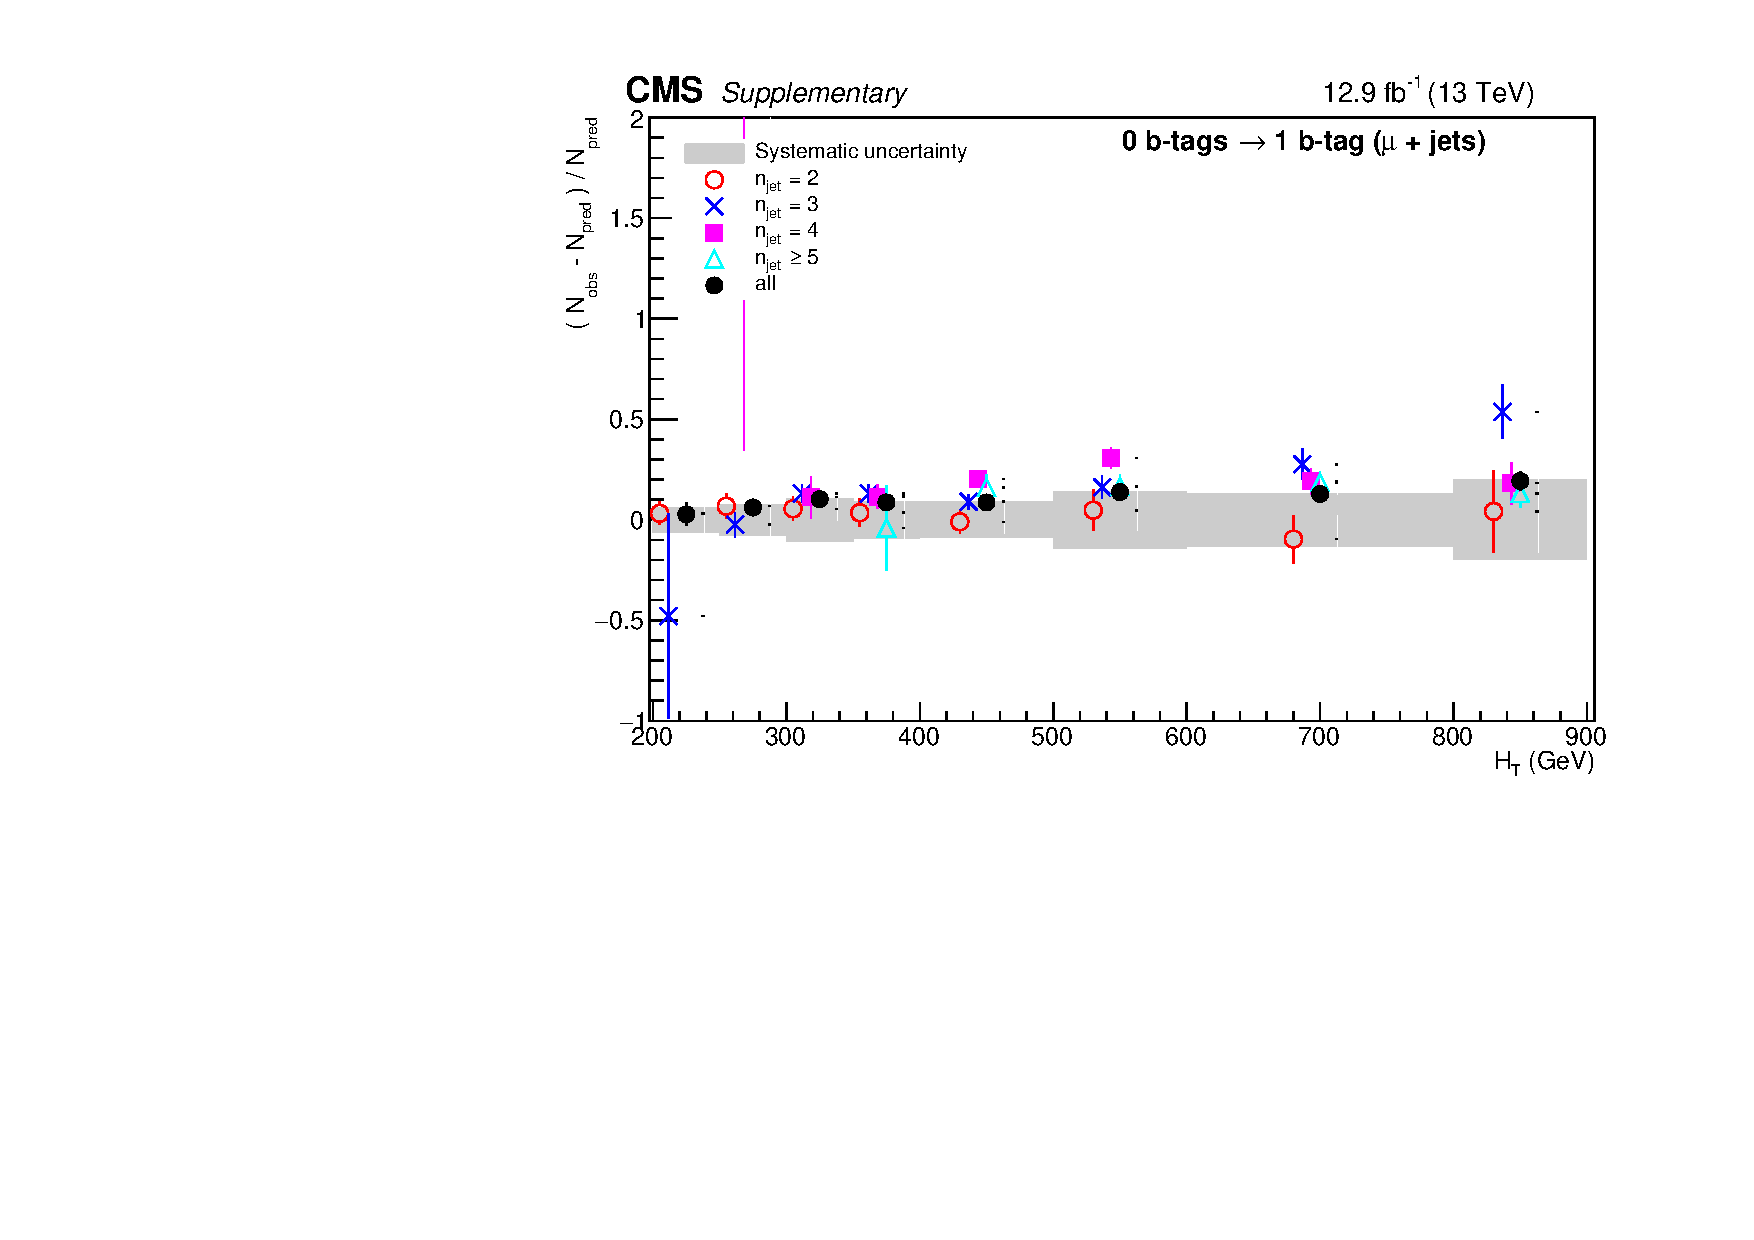
\includegraphics[width=0.5\textwidth]{figs/analysis/closureTests/eq0b_eq1b_muon_sym__noFit.pdf}}
    ~~
    \subfloat[]{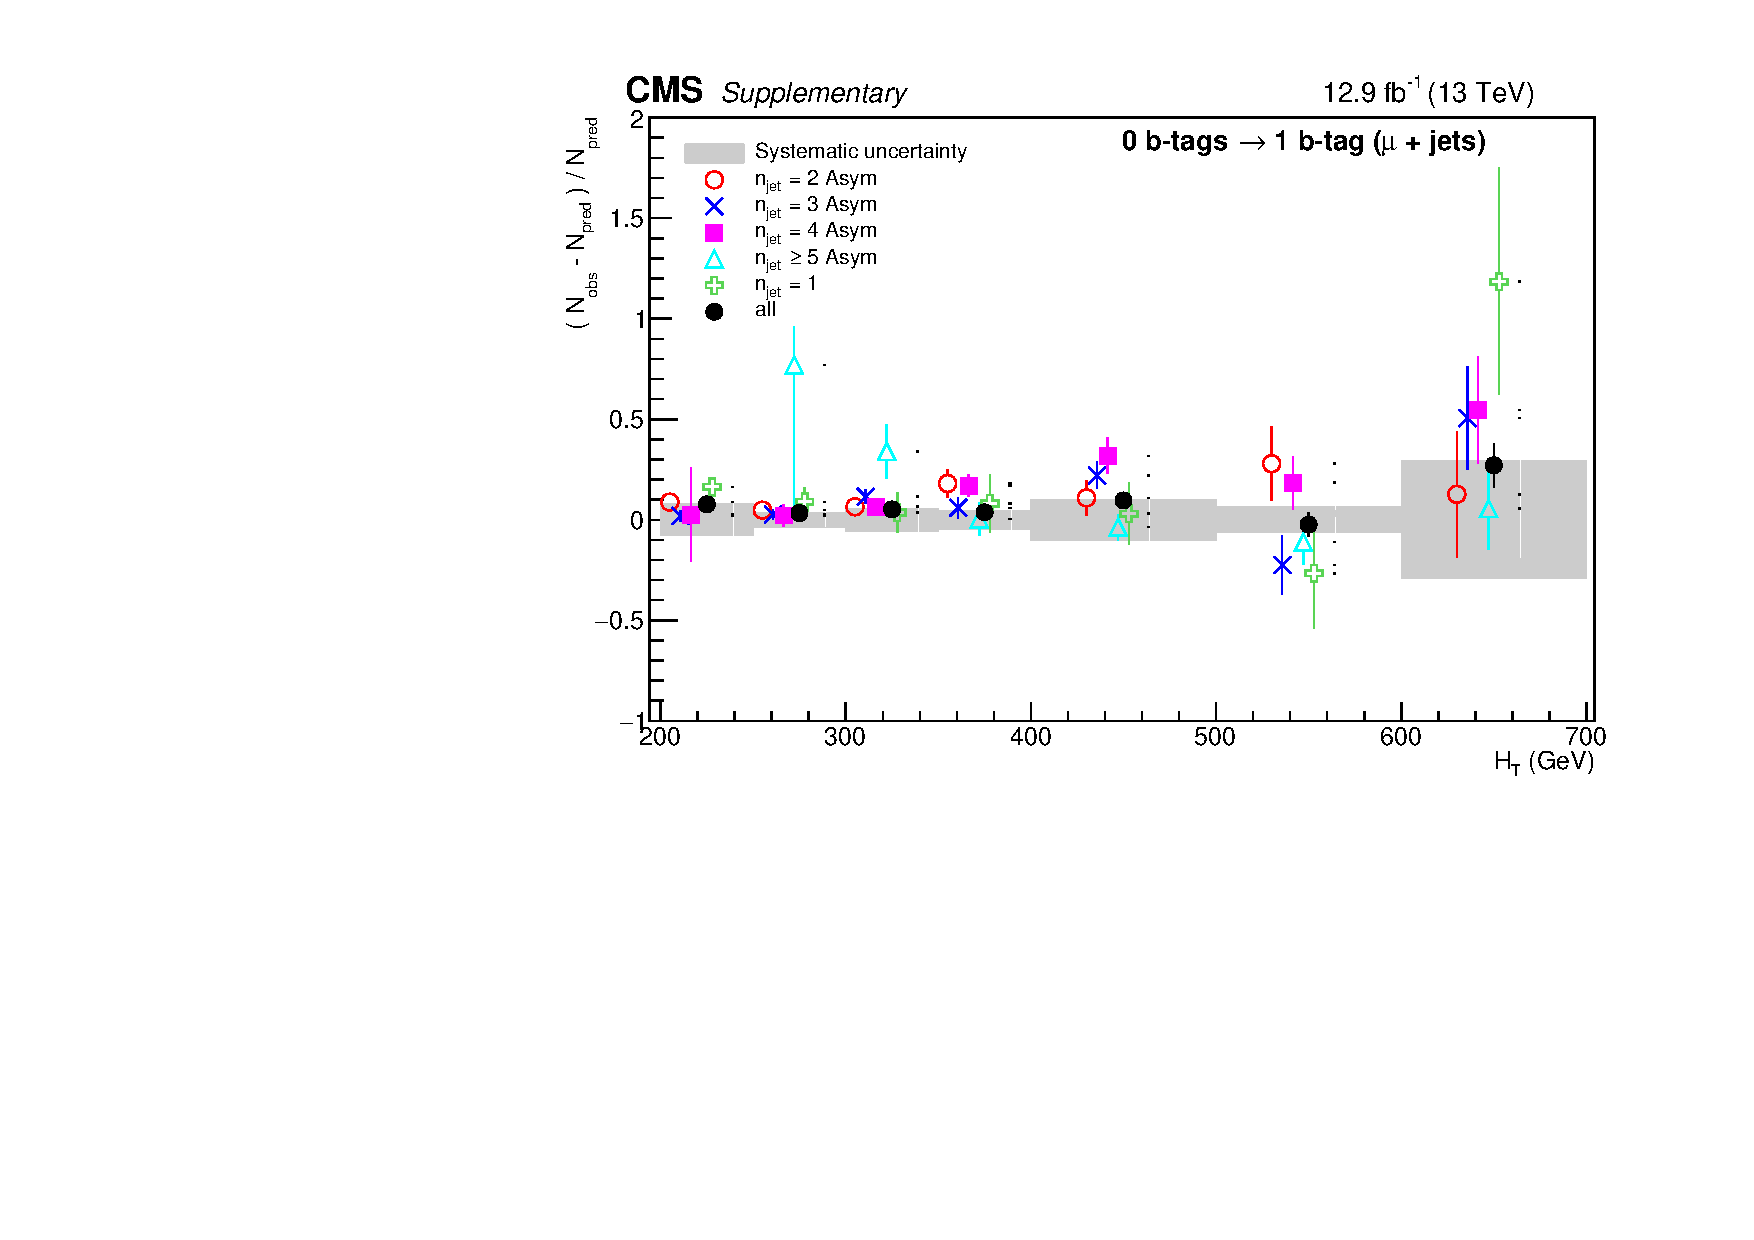
\includegraphics[width=0.5\textwidth]{figs/analysis/closureTests/eq0b_eq1b_muon_asym__noFit.pdf}} 
    \caption{Data-driven tests probing the W and \ttbar admixture 
      in each \njet category (open symbols) overlaid on top of the systematic
      uncertainty estimates used for each of the seven \scalht bins
      (shaded bands). 
      The symmetric (asymmetric) jet topologies are shown in the left (right) plot.      
    }
    \label{fig:closureBTag}
  \end{center} 
\end{figure}

\subsection{Uncertainties in the \MHT dimension}
\label{sec:systMht}

Along with the uncertainty on the \TFs, described above, additional
uncertainties in the shape of the \MHT distribution that is taken from
simulation are derived. For all the known sources of systematic
uncertainty, discussed in Sec.~\ref{sec:simUnc}, the effect of the $\pm 1\sigma$
variation is propagated as uncertainty that varies the \MHT shape.
Due to the fact that the analysis is binned in \HT and \nj bin
migration effects are minimised and these sources of uncertainty are
found to be subdominant.

There is also an uncertainty associated with the fact that the \MHT shape
is taken directly from simulation. To estimate this, a data-driven
method is devised, based on the validation of the \MHT shapes
described in Sec.~\ref{sec:mhtDim}. Within the \mj, \mmj and \gj
control regions the data-simulation ratio of the \MHT shape is
constructed for each (\HT,\nj,\nb) bin. The agreement between the two
distributions is parameterised with a linear orthogonal polynomial.
This function is chosen as it allows one to make a linear fit with
just one parameter as the total overall normalisation is preserved.
To derive the uncertainty for each of the background sources
a simultaneous fit of the \MHT shapes is performed across
all the relevant control regions. This gives a value for the fit
parameter, $p$, which should be compatible with flat, i.e.
$p\approx0$. The uncertainty is then taken as the quadrature sum of
the value of $p$ with its one sigma deviation. This allows alternative
\MHT shapes to be derived based on the $\pm 1\sigma$ variation of this
uncertainty. These alternative shapes are used to encode the
data-driven uncertainty when it is propagated to the final result. An
example of the kind of fit that occurs in a particular bin was shown
in Fig.~\ref{fig:linearFitExamples}. The uncertainty of the linear fit is shown as a red
shaded region.

The size of the systematic uncertainty for the data-driven orthogonal
polynomial variation and the sources of known systematic uncertainties
for one of the extremal analysis categories is shown in
Fig.~\ref{fig:mcCompLow}.
The upwards and downward variation for each of the labelled sources
are plotted for a normalised \MHT shape. The data-driven systematic
dominates over other sources.

\begin{figure}[h!]
  \centering
  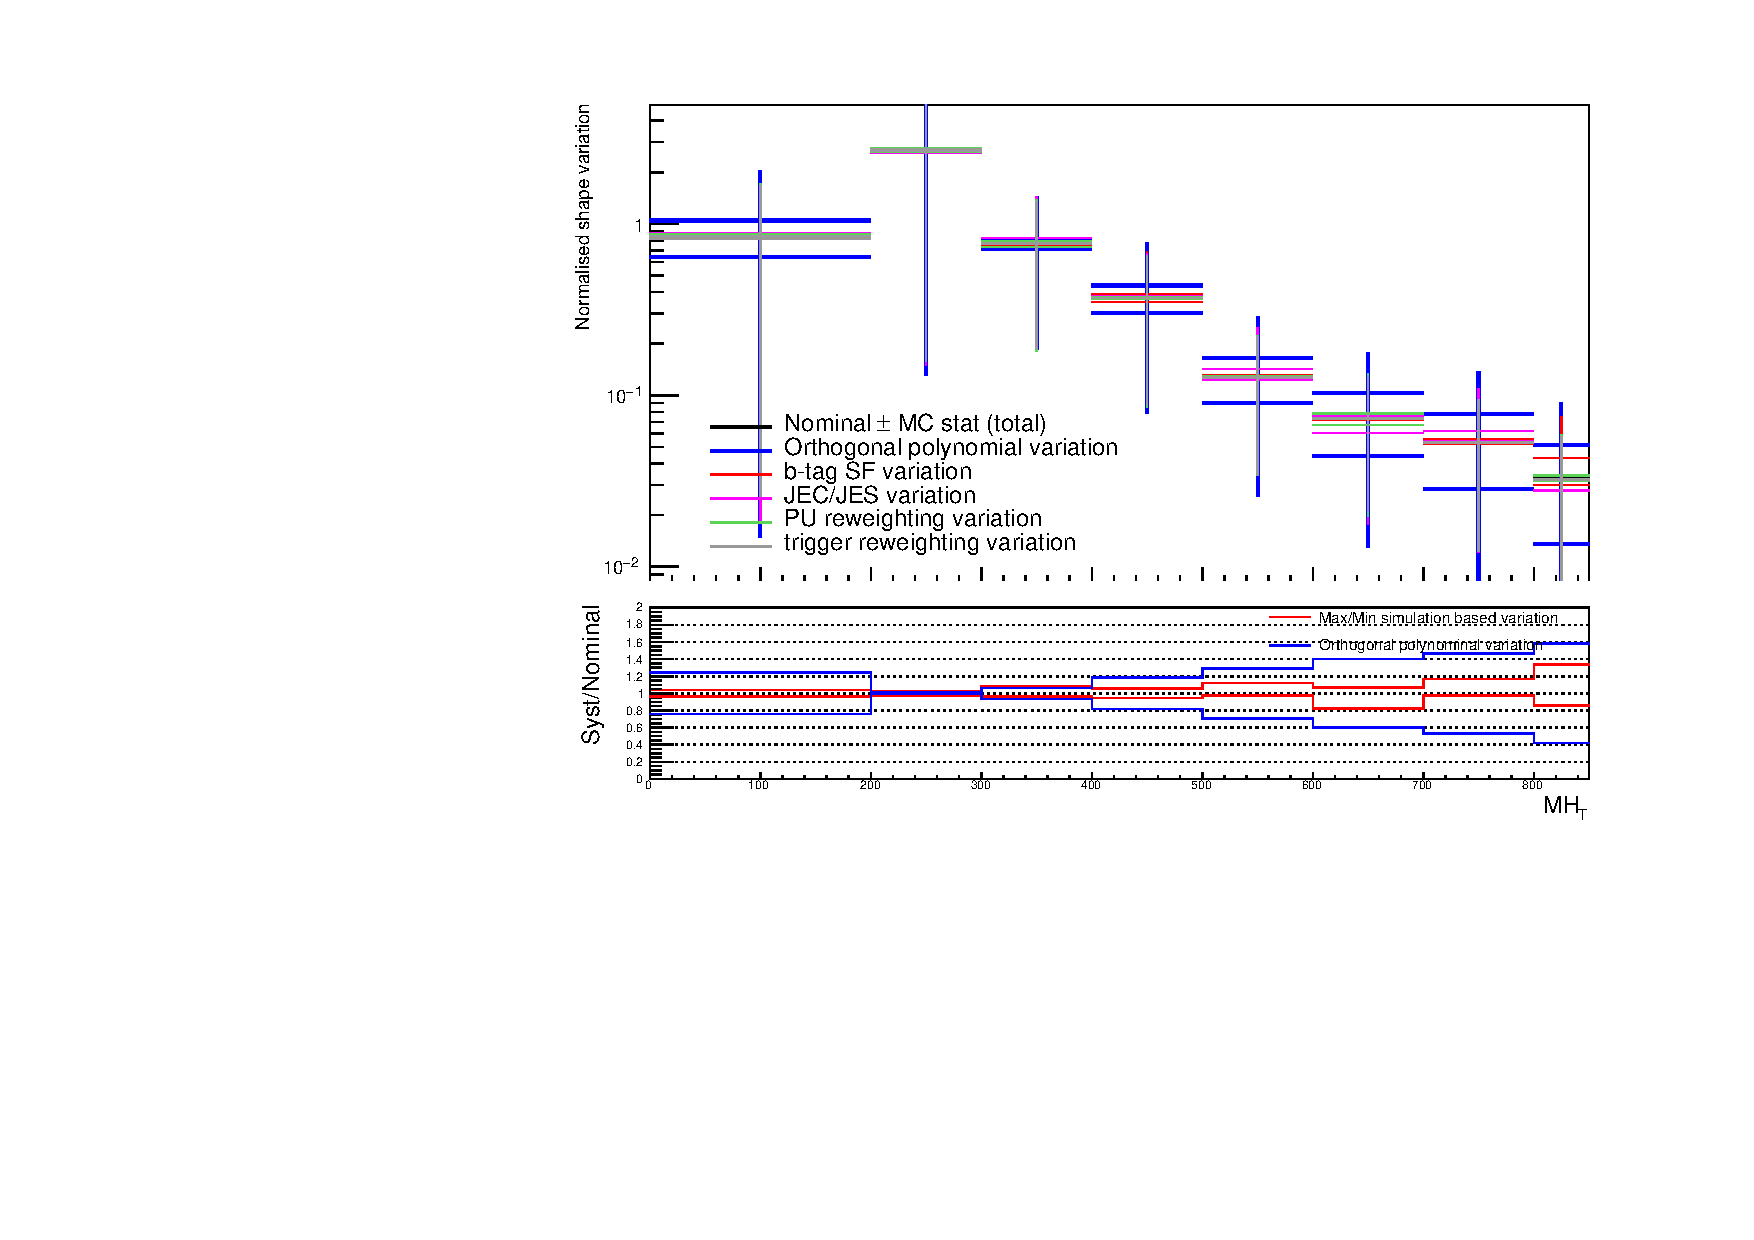
\includegraphics[width=0.8\textwidth]{figs/analysis/mhtShape/totalSMS-T1tttt_mGluino-1000_mLSP-100_25ns_mht_ge5j_ge3b_800.pdf}
  \caption{The systematic variation of the normalised \MHT (denoted MH$_T$)
  distribution for an array of uncertainties derived from simulation
  and a data driven \emph{orthogonal polynomial variation} in the
  extremal analysis category: \scalht $800-\infty$, \njet $\geq 5$, \nb $\geq 2$.}
  \label{fig:mcCompLow}
\end{figure}

\newpage
\begin{landscape}
\begin{table}[h!]
  \caption{Summary of the systematics on the transfer factors considered in the analysis, 
    with representatives ranges of uncertainties and the correlation assummed, 
    for the predictions of the $\ttbar$, W and $\znunu$  background
    components.}
  \label{tab:systs}
  \centering
  \footnotesize
  \begin{tabular}{ ccccccc }
    \hline
    \hline
    Systematic & Method & \multicolumn{4}{c}{Relative uncertainty on transfer factor} & Correlation model \\    
     & & $\mj \rightarrow$  & $\mmj \rightarrow$ & $\gj \rightarrow$ & $\mj \rightarrow$ & \\
     & & $\znunu$  & $\znunu$ & $\znunu$ & $\ttbar+W$ & \\
    \hline
    \alphat/\bdphi extrapolation & data-driven tests & $3-30\%$ & $3-30\%$ & - & $3-30\%$ & un-correlated across \scalht/jet top. \\
    W/Z ratio & data-driven tests & $4-15\%$ & - & - & - & un-correlated across \scalht/jet top. \\
    Z/$\gamma$ ratio & data-driven tests & - & - & $6-11\%$ & - & un-correlated across \scalht/jet top. \\
    W/\ttbar admixture & data-driven tests & - & - & - & $4-30\%$ & un-correlated across \scalht/jet top. \\
    W polarisation & data-driven tests & $2-10\%$ & - & - & $2-10\%$ & un-correlated across \scalht/jet top. \\
    Jet energy scale & MC variations & $1-5\%$ & $1-5\%$ & $1-5\%$ & $1-5\%$ & fully correlated \\
    B-tagging efficiency b and c jets & MC variations & $1-3\%$ & $1-3\%$ & $1-3\%$ & $1-3\%$ & fully correlated \\
    B-tagging efficiency light jets & MC variations & $1-3\%$ & $1-3\%$ & $1-3\%$ & $1-3\%$ & fully correlated \\
    Pileup weights & MC variations & $0-2\%$ & $0-2\%$ & $0-2\%$ & $0-2\%$ & fully correlated \\
    Top $p_{T}$ weights & MC variations & $1-30\%$  & $1-10\%$ & - & $1-10\%$ & fully correlated \\
    Lepton scale factor & MC variations & $1-3\%$ & $1-3\%$ & - & $1-3\%$ & fully correlated \\
    Signal trigger efficiency & MC variations & $1-2\%$ & $1-2\%$ & $1-2\%$ & $1-2\%$ & fully correlated \\
    Photon trigger efficiency & MC variations & - & - & $1-2\%$ & - & fully correlated \\
    \hline
    \hline
  \end{tabular}
\end{table}

\end{landscape}


%%%%%%%%%%%%%%%%%%%%
\section{The likelihood model}  % day 3
\label{sec:likelihood}

To carry out a full interpretation of the results of the analysis with
appropriate treatment of systematic uncertainties, a likelihood model
is constructed. Events are categorised based on their (\HT,\nj,\nb)
bin, labelled \htcat, in both the signal region and control regions. Additionally, the
signal region is categorised based on the \MHT bins discussed in
Sec.~\ref{sec:mhtDim}. These bins are represented with an additional
index, $i$. Given
that $n^{\htcat}_{\mathrm{had},i}$ is the number of observed events,
$b^{\htcat}_{\mathrm{had},i}$ is the number of predicted background
events and $s^{\htcat}_{\mathrm{had},i}$ is the expected number of
signal events, the likelihood function in each \htcat category is
defined as the product of poisson distributions for each \MHT bin:
% had likelihood
\begin{equation}
\mathcal{L}^{\htcat}_{\mathrm{had}}=\prod_i
\mathrm{Poisson}(n^{\htcat}_{\mathrm{had},i} |\,
b^{\htcat}_{\mathrm{had},i} + s^{\htcat}_{\mathrm{had},i}).
\label{eq:hadronicLikelihood}
\end{equation}

For each control region, indexed $j$, an independent likelihood
function can be constructed, given $n^{\htcat}_{\mathrm{CR},j}$ is
the number of observed events, $b^{\htcat}_{\mathrm{CR},j}$ is the
number of predicted background events and
$s^{\htcat}_{\mathrm{had},j}$ is the expected signal contamination in
the control region:
% CR likelihood
\begin{equation}
\mathcal{L}^{\htcat}_{\mathrm{CR,j}}=\mathrm{Pois}(n^{\htcat}_{\mathrm{CR,j}}
|\, b^{\htcat}_{\mathrm{CR,j}} + s^{\htcat}_{\mathrm{CR,j}}).
\label{eq:controlLikelihood}
\end{equation}
Due to the way the control regions are selected, the expected signal
contamination is usually found to be negligible.

This results in a total likelihood that is the product over all the
\htcat bins and all the control regions. It can be defined as:
% combined likelihood
\begin{equation}
\label{eq:total_likelihood}
\mathcal{L} = \prod_{\htcat} (\mathcal{L}_{\text{had}}^{\htcat} \times
\prod_{\text{j}} \mathcal{L}_{\text{CR,j}}^{\htcat})
\end{equation}

\subsection{Incorporation of systematic uncertainties}

The background yields in the signal region are connected to the yields
in the control regions through the use of \TFs, as discussed in
Sec.~\ref{sec:TF}. To incorporate this into the fit of the likelihood
model, the yields of the \znunu and combined W+\ttbar backgrounds in
the signal region are correlated with the yields in the control
regions. This is implemented through a single floating parameter
within the fit, which alters the background prediction in the signal
region based on the control region yields and the \TF for each
category. With this implementation, the systematic uncertainties on
each \TF can be properly taken into account when making the background
prediction in the signal region. 

The data-driven uncertainties on the \TFs, described in
Sec.~\ref{sec:closureTests}, are incorporated into the likelihood
model as Gaussian distributed nuisance parameters that act on the
floating parameter. They depend on the background process and the
control region used and are uncorrelated between each of the \htcat
bins.

The uncertainties on the \TFs determined from simulation, described in
Sec.~\ref{sec:simUnc}, are included as \emph{shape} uncertainties on
the \TFs. This means they are fully correlated across all of the
\htcat bins but their magnitude is different depending on the bin. 
Additionally, an uncertainty on the expected signal contribution can
also be taken account of with shape uncertainties. These extra
uncertainties depend on the signal model in question and are discussed
in Sec.~\ref{sec:signalModel}.

The uncertainties derived from simulation can also cause bin migration
of events within the \MHT dimension of the signal region. This is
incorporated as a \emph{template} uncertainty, i.e. alternative \MHT
distributions for the $\pm1\sigma$ variation for each of the sources
of uncertainty. 

% (checked this is correct with Matt - depends on the
% analysis, for ICHEP do a simulataneous fit separately for Zinv and
% ttW, uncertainty made from adding p1 in quadrature to p1 unc)
To take account of the uncertainties in the \MHT
distribution, explained in Sec.~\ref{sec:systMht}, additional template
uncertainties are introduced that are decorrelated in \nj and \HT.
Their $\pm1\sigma$ is determined by the uncertainty on the linear fit
used when determining the magnitude of the \MHT uncertainty.
% what about other MHT problem?

Finally, the uncertainty from the limited statistical power of the \MC
samples used is incorporated as an additional nuisance parameter per
\htcat and \MHT bin. This is taken as uncorrelated across all bins.

\subsection{Fitting}

The fit of the likelihood model to find the final result is carried
out in two steps. Firstly, the predicted background yields in the
signal region, $b^{\htcat}_{\mathrm{had}}$, are determined with a fit
in only the control regions, Eq.~\ref{eq:controlLikelihood}. This is
followed by a full fit using the full likelihood model,
Eq.~\ref{eq:total_likelihood}, taking account of all the correlations
between the control regions and signal region, along with the
statistical uncertainties from the
finite number of events in the control region. Within the fit the
likelihood is profiled against all nuisance parameters, which allows
the determination of limits on various signal models. This is
discussed further in Sec.~\ref{sec:signalModel}.

% how the fit is done - split into two components

